
% %\documentclass[12pt,fleqn]{exam}
% \documentclass[12pt]{exam}

% \usepackage[margin=0.75in]{geometry}

% %\usepackage{geometry}                % See geometry.pdf to learn the layout options. There are lots.
% %\geometry{letterpaper}                   % ... or a4paper or a5paper or ... 
% %\geometry{landscape}                % Activate for for rotated page geometry
% %\usepackage[parfill]{parskip}    % Activate to begin paragraphs with an empty line rather than an indent
% \usepackage{graphicx}
% \graphicspath{ {./images/} }

% \usepackage{subfig}
% \usepackage{amssymb}
% \usepackage{epstopdf}
% \usepackage{multicol}
% \usepackage{amsmath}
% \usepackage{enumitem}
% \usepackage{pifont}
% \usepackage{bbding}

% \usepackage{array}
% \usepackage{xcolor}
% \usepackage{colortbl}


% %\usepackage{fontspec}
% %\usepackage{fontspec}
% \usepackage[all]{background}
% \usepackage{textcomp}
% \usepackage{xcolor}
% \usepackage[most]{tcolorbox} % Load the tcolorbox package
% \usepackage[makeroom]{cancel}
% \usepackage{tikz, pgfplots, pgfmath, pgffor, amssymb}
% \usetikzlibrary{matrix}
% \usepackage{tkz-tab}
% \usepackage{xpatch}
% % tkz-tab hardcodes $0$ for the zeros
% \xpatchcmd{\tkzTabLine}{$0$}{$\bullet$}{}{}
% % we want solid lines
% \tikzset{t style/.style={style=solid}}

% \usetikzlibrary{arrows}
% \usepackage{mathtools} % Required for \Aboxed
% \usepackage{caption} % Required for caption customization
% \usepackage{subcaption} % Required for subfigures
% \newcommand{\hh}[1]{{\textcolor{red}{#1}}}
% \newcommand{\kk}[1]{{\textcolor{cyan}{#1}}}
% \newcommand{\rr}[1]{{\textcolor{brown}{#1}}}
% \newcommand{\notebox}[1]{\colorbox{yellow!30}{#1}}






% %\setmainfont{QTKorrin}
% %\setmainfont{savedbyzero.ttf}
% % Set your main document font
% %\setmainfont{EB Garamond}

% %Optionally, set a different font for sans-serif text
% %\setsansfont{Fira Sans}

% \pagestyle{headandfoot}
% \firstpageheader{}{Questions}{}
% \firstpageheadrule
% \runningheadrule
% \firstpagefooter{\textcopyright\ 2025 B2B STEM}{Page \thepage\ of \numpages}{All Rights Reserved}
% \runningfooter{\textcopyright\ 2025 B2B STEM}{Page \thepage\ of \numpages}{All Rights Reserved}

% %\DeclareGraphicsRule{.tif}{png}{.png}{`convert #1 `dirname #1`/`basename #1 .tif`.png}
% % Configure the watermark
% \backgroundsetup{
%   opacity=0.01, % Adjust the transparency (0-1)
%   scale=0.65,   % Adjust the image size
%   angle=45,     % Angle of the image (0 = no rotation)
%   contents={\includegraphics[width=\paperwidth, height=\paperheight, keepaspectratio]{images/wm1}}
% }


% \title{Logarithms}

% % \author{\newfontfamily{\myspecialfont}{savedbyzero.ttf} % Define the new font family
% % \myspecialfont % Apply the new font family
% % B2B STEM 
% % \endgroup} % End the group, reverting to the previous font}


% %\date{}                                           % Activate to display a given date or no date
% \printanswers 


% \begin{document}
% \maketitle
% \large{
% \noindent 
% Dear Teachers and Students,\\


% \noindent
% This booklet offers problems on systems of equations with two and three variables. The "solutions" and video packages include graphing, substitution, elimination, and matrix methods such as Cramer's Rule and row operations, just to name a couple. To maximize your learning, try solving the problems before reviewing the solutions. This approach will enhance your aptitude in the subject matter and better prepare you for both in-class and standardized tests.\\

% \noindent
% Additionally, a video solutions package is available, featuring 10 solved problems that are representative of the problem set in this booklet. In these videos, we thoroughly work through each problem and explain my approach to finding the solution.\\
% \noindent


% Please note that this worksheet is designed for practice and reinforcement, not as an initial lesson on the material. We assume that you are already familiar with these concepts from lectures and classes. The purpose of these problems is to help you solidify your understanding and master the material through varied difficulty levels.\\

% \noindent
% Thank you for supporting our work. We hope that you find this resource valuable. Please share your feedback and suggestions with us using the form provided on our page.\\


% \noindent
% Sincerely,\\
% B2B STEM Team
% % \begingroup % Start a new group to limit the scope of the font change
% % \newfontfamily{\myspecialfont}{savedbyzero.ttf} % Define the new font family
% % \myspecialfont % Apply the new font family
% % B2B STEM Team
% % \endgroup % End the group, reverting to the previous font


% }\\
% % %\textcopyright\ 2025 B2B STEM. All Rights Reserved.
% % \newpage
% % \begin{center}
% % \fbox{\begin{minipage}{0.9\textwidth}
% % \centering
% % \textbf{\large COPYRIGHT AND USAGE NOTICE}
% % \vspace{0.3cm}

% % \textcolor{red}{\textbf{RESTRICTED MATERIAL - FOR AUTHORIZED USE ONLY}}
% % \vspace{0.2cm}

% % \textbf{Copyright Notice:} This educational material is protected by copyright law. All rights reserved.
% % \vspace{0.1cm}

% % \textbf{Usage Restrictions:}
% % \begin{itemize}
% % \item This worksheet/pamphlet is licensed exclusively for use by the original purchaser.
% % \item \textbf{Distribution, reproduction, copying, or sharing of this material is strictly prohibited} without explicit written permission from the author.
% % \item This includes but is not limited to: photocopying, digital copying, email distribution, posting online, or any other form of redistribution.
% % \item Each copy must be individually purchased and licensed.
% % \item Violation of these terms may result in legal action for copyright infringement.
% % \end{itemize}

% % \textbf{Permitted Use:}
% % \begin{itemize}
% % \item Personal educational use by the purchaser only
% % \item Use in the purchaser's classroom with their own students (if applicable)
% % \item Making personal notes or annotations on your copy
% % \end{itemize}

% % \vspace{0.1cm}
% % \textit{For licensing inquiries or permission requests, please contact the author.}
% % \vspace{0.1cm}

% % \textbf{By using this material, you acknowledge that you have read, understood, and agree to comply with these terms and conditions.}
% % \end{minipage}}
% % \end{center}
% % \newpage

% % % Copyright and Usage Restrictions
% % \begin{center}
% % \fbox{\begin{minipage}{0.9\textwidth}
% % \centering
% % \textbf{\large COPYRIGHT AND USAGE NOTICE}
% % \vspace{0.3cm}

% % \textcolor{red}{\textbf{PERSONAL USE ONLY - NO DISTRIBUTION PERMITTED}}
% % \vspace{0.2cm}

% % \textbf{Copyright Notice:} This educational material is protected by copyright law. All rights reserved.
% % \vspace{0.1cm}

% % \textbf{STRICT USAGE RESTRICTIONS:}
% % \begin{itemize}
% % \item \textbf{THIS MATERIAL IS FOR PERSONAL USE BY THE PURCHASER ONLY}
% % \item \textbf{NO sharing, distribution, reproduction, or copying is permitted under any circumstances}
% % \item \textbf{NO classroom use, tutoring use, or educational institution use without separate licensing}
% % \item \textbf{NO photocopying, scanning, digital copying, or any form of duplication}
% % \item \textbf{NO email sharing, online posting, cloud sharing, or electronic distribution}
% % \item \textbf{NO lending, gifting, or transferring to any other person or entity}
% % \item Each individual user must purchase their own separate license
% % \item Violation of these terms will result in immediate legal action for copyright infringement
% % \end{itemize}

% % \textbf{PERMITTED USE - PERSONAL ONLY:}
% % \begin{itemize}
% % \item Individual study and practice by the purchaser exclusively
% % \item Making handwritten personal notes on your individual copy only
% % \item \textbf{NO OTHER USE IS AUTHORIZED}
% % \end{itemize}

% % \vspace{0.1cm}
% % \textbf{\textcolor{red}{IMPORTANT:}} Teachers, tutors, and educational institutions must purchase separate commercial licenses.
% % \vspace{0.1cm}

% % \textit{For commercial licensing inquiries, please contact the author.}
% % \vspace{0.1cm}

% % \textbf{By using this material, you acknowledge that you have read, understood, and agree to comply with these strict terms and conditions. Any violation constitutes copyright infringement and will be prosecuted to the full extent of the law.}
% % \end{minipage}}
% % \end{center}


% \newpage

% % Copyright and Usage Restrictions
% \begin{center}
% \fbox{\begin{minipage}{0.9\textwidth}
% \centering
% \textbf{\large COPYRIGHT AND USAGE NOTICE}
% \vspace{0.3cm}

% \textcolor{blue}{\textbf{Personal Use License}}
% \vspace{0.2cm}

% \textbf{Copyright Notice:} This educational material is protected by copyright law. All rights reserved.
% \vspace{0.1cm}

% \textbf{What You Can Do (Personal Use):}
% \begin{itemize}
% \item Use this material for your own personal study and practice
% \item Print copies for your personal use only
% \item Make handwritten notes and annotations on your copies
% \item Store digital copies on your personal devices for your own use
% \end{itemize}

% \textbf{Usage Limitations:}
% \begin{itemize}
% \item This license is for personal use by the purchaser only
% \item Please do not share, distribute, or copy this material for others
% \item Commercial use (including classroom teaching, tutoring, or institutional use) requires a separate license
% \item Please do not post online, email to others, or upload to shared platforms
% \item Each person who wants to use this material should purchase their own copy
% \end{itemize}

% \vspace{0.1cm}
% \textit{For teachers, tutors, and educational institutions: Please contact us about our educational licensing options.}
% \vspace{0.1cm}

% \textbf{We appreciate your understanding and respect for our work. By using this material, you agree to these reasonable terms.}
% \end{minipage}}
% \end{center}


% .\par
% \setlength{\columnsep}{2.5cm} % Set the gap between columns
% %\setlength{\columnseprule}{0.5pt} % Add a thin vertical rule


% \newpage

\chead{Problems}

\section*{Properties and Rules}
\chead{Logarithm Properties and Rules}

\begin{multicols}{2}
\noindent
\textbf{Definition:}\\ $\log_{10}(x)=\log(x); \log_e(x)=\ln(x)$\\

\vspace{0.2in}\noindent
\textbf{Definition:} $\log_bx=y\Leftrightarrow x=b^y$\\
Example: $\log_3x=7\Leftrightarrow x=3^7$\\
\end{multicols}

\begin{multicols}{2}
\vspace{0.2in}\noindent
\textbf{Zero:} $\log_b1 = 0$\\
Example: $\log_31=0;\quad\log_{1/2}1=0$\\

\vspace{0.2in}\noindent
\textbf{Identity:} $\log_b b=1$\\
Example: $\log_44=1;\quad\log_{\frac{3}{2}}\frac{3}{2}=1$\\

\vspace{0.2in}\noindent
\textbf{Power:} $\log_bx^n=n\log_bx$\\
Example:\\
$\log_27^3=3\log_27$\\
$\quad\log_3x^{-3}=-3\log_3x$\\

\vspace{0.2in}\noindent
\textbf{Inverse:} $\log_b b^u=u$\\% ;\quad b^{\log_bu}=u$ \\
Example: $\log_2 2^5=5$\\%;\quad 3^{\log_37}=7$\\

\vspace{0.3in}\noindent
\textbf{Product:}\\
$\log_b(u w) = \log_bu+\log_bw$\\
Example:$\log_3(2x) = \log_32+\log_3x$ \\

\vspace{0.2in}\noindent
\textbf{Quotient:} $\log_b(\frac{u}{w}) = \log_bu-\log_bw$\\
Example: $\log_6(\frac{7}{8}) = \log_67-\log_68$\\

\vspace{0.2in}\noindent
\textbf{Change of Base:} $\log_ba=\frac{\log_ca}{\log_cb}$\\
%\Rightarrow\log_ca=\log_cb\log_ba$\\
Example:$\log_32=\frac{\log_52}{\log_53}$%\Rightarrow\log_52=\log_53\log_32$\\

\vspace{0.2in}\noindent
\textbf{Equality of Base :}\\ $\log_bu=\log_bw\Leftrightarrow u=w$\\
Example: $\log_2x=\log_27\Leftrightarrow x=7$\\
\end{multicols}


% %%%%%%%%%%%%%%%%%%%%%%%%%%%%%%%%%%%%%%%%%%%%%%%%%%%%%%%%%%%%%%%%%%%%%%%%%%%%%%%
%%%
%%%                     New Properties
%%%
%%%%%%%%%%%%%%%%%%%%%%%%%%%%%%%%%%%%%%%%%%%%%%%%%%%%%%%%%%%%%%%%%%%%%%%%%%%%%%%





\newpage
\chead{Problems}
% Optional: add a clearpage if you want the text on its own page
\clearpage 

% Vertical centering: moves the content to the middle of the page
\vspace*{\fill} 

% Horizontal centering: centers the text block horizontally
\begin{center} 
  % Set a very large font size (e.g., 50pt with 60pt line spacing)
  {\fontsize{70}{60}\selectfont 
  \textbf{P R O B L E M S}
  }
\end{center}

% Vertical centering: balances the 'vspace' above
\vfill 

% Optional: add another clearpage to prevent subsequent text from appearing on the same page
 \clearpage

\newpage
\subsection*{Show That The Statements Are True}

\begin{enumerate}
\item $\log_ac\cdot\log_cb=\log_ab$
\item $\log_b{1/a}=-\log_b{a}$
\item $\log_ax=-\log_{1/a}x$
\item $\log_{m^n}x^y=\frac{y}{n}\,\log_mx$
\end{enumerate}
%%%%%%%%%%%%%%%%%%%%%%%%%%%%%%%%%%%%%%%%%%%%%%%%%%%%%%%%%%%%%%%%%%%%%%%%%%%%%%%
%%%
%%%                     WRITE IN LOGARTHMIC FORM
%%%
%%%%%%%%%%%%%%%%%%%%%%%%%%%%%%%%%%%%%%%%%%%%%%%%%%%%%%%%%%%%%%%%%%%%%%%%%%%%%%%
\subsection*{Write In Logarithmic Form}
\begin{enumerate}[resume]

\item $\left(\dfrac{1}{6}\right)^{-3}=216$
\item $5^{3}=125$
\item $10^{-4}=0.001$
\item $e^4=x-1$
\item $z^3=v$
\item $10^6=1,000,000$
\end{enumerate}

%%%%%%%%%%%%%%%%%%%%%%%%%%%%%%%%%%%%%%%%%%%%%%%%%%%%%%%%%%%%%%%%%%%%%%%%%%%%%%%
%%%
%%%                     EVALUATE WIHTOUT USING A CALCULATOR
%%%
%%%%%%%%%%%%%%%%%%%%%%%%%%%%%%%%%%%%%%%%%%%%%%%%%%%%%%%%%%%%%%%%%%%%%%%%%%%%%%%
\subsection*{Evaluate without using a calculator}
\begin{enumerate}[resume]

\item $\log_3(9)$
\item $\log_5(25) + \log_5(5)$
\item $\log_2(8)$
\item $\log_{10}(100)$
\item $\log_5(1)$
\item  $\log_7(7)$
\item  $\log_2(4) + \log_2(8)$
\item  $\log_3(27) - \log_3(3)$
\item $2\log_5(5)$
\item $\log_{10}(1000)$
\item $\log_3(\log_2(\log_2(256)))$
\end{enumerate}

%%%%%%%%%%%%%%%%%%%%%%%%%%%%%%%%%%%%%%%%%%%%%%%%%%%%%%%%%%%%%%%%%%%%%%%%%%%%%%%
%%%
%%%                     FIND THE DOMAIN AND ASYMPTOTES
%%%
%%%%%%%%%%%%%%%%%%%%%%%%%%%%%%%%%%%%%%%%%%%%%%%%%%%%%%%%%%%%%%%%%%%%%%%%%%%%%%%
\subsection*{Identify The Domain and Any Vertical Asymptote(s)}

\begin{enumerate}[resume]

\item $y=\log_2(x-3)$  
\item $y=\ln(x^2-16)$
\item $y=\log(x^2+5x+6)$
\item $y=\log\left(\sqrt{2x-1}+2\right)$
\item $y=\ln\left(\dfrac{2-x}{\sqrt{x+4}}\right)$
\item $y=\log_2(x^2+1)-3x$
\item $y=\log(x+3)^2$
\item $y=\log\left(\dfrac{x-3}{x+2}\right)$
\item $y=\ln\left(\sqrt{x-2}-1\right)$
\end{enumerate}

%%%%%%%%%%%%%%%%%%%%%%%%%%%%%%%%%%%%%%%%%%%%%%%%%%%%%%%%%%%%%%%%%%%%%%%%%%%%%%%
%%%
%%%                     PLOT USING TRANSFORMATIONS
%%%
%%%%%%%%%%%%%%%%%%%%%%%%%%%%%%%%%%%%%%%%%%%%%%%%%%%%%%%%%%%%%%%%%%%%%%%%%%%%%%%
\section*{Plot Using Transformations}
\begin{enumerate}[resume]

\item $f(x)=\log_2(x-3)$
\item $f(x)=\log_3(1+x)+2$   
\item $f(x)=4-2\ln(x+2)$
\item $f(x)=4-\log(4-x)$
\item $y=3\log_2(2x+1)-2$
\end{enumerate}

%%%%%%%%%%%%%%%%%%%%%%%%%%%%%%%%%%%%%%%%%%%%%%%%%%%%%%%%%%%%%%%%%%%%%%%%%%%%%%%
%%%
%%%                     EXPAND COMPLETELY
%%%
%%%%%%%%%%%%%%%%%%%%%%%%%%%%%%%%%%%%%%%%%%%%%%%%%%%%%%%%%%%%%%%%%%%%%%%%%%%%%%%
\subsection*{Expand Completely}
\begin{enumerate}[resume]

\item $\log_4(x^3)$
\item $\log_7(49x)$
\item $\log_2(5xy)$
\item  $\log_{10}(x^2y^3)$
\item  $\log_2\left(\dfrac{x^3y^2}{z^4}\right)$
\item $\log\left(\dfrac{\sqrt{f^2-3}}{1000}\right)$
\item  $\log_3\left(\dfrac{x^2\sqrt[3]{y}}{(z+1)^4}\right)$
\item  $\log_7\left(\dfrac{\sqrt{x}}{y^2z}\right)$
\item  $\log_{e}\left(\dfrac{x^2\sqrt{y}}{z^3}\right)$
\item $\log_4\left(\dfrac{x^3\sqrt[4]{y^3}}{(z^2+1)^{3/2}}\right)$
\end{enumerate}

%%%%%%%%%%%%%%%%%%%%%%%%%%%%%%%%%%%%%%%%%%%%%%%%%%%%%%%%%%%%%%%%%%%%%%%%%%%%%%%
%%%
%%%                     EXPRESS AS A SINGLE LOGARITHM
%%%
%%%%%%%%%%%%%%%%%%%%%%%%%%%%%%%%%%%%%%%%%%%%%%%%%%%%%%%%%%%%%%%%%%%%%%%%%%%%%%%
\subsection*{Express as a single logarithm (when possible)}
\begin{enumerate}[resume]

\item  $\log_3(5) + \log_3(7)$
\item  $\log_2(12) - \log_2(3)$
\item $\dfrac{1}{2}\log(z)-\log(z-5)+\log(z^2-25)$
\item $\dfrac{2}{3}\left( 2\ln(x-1)+\ln x-\ln(x^2-9)-3\ln(x+1)\right)$
\item $2\log_5(3)$
\item $\log_6(8) + \log_6(2) - \log_6(4)$
\item $3\log_4(2) + \log_4(5)$
\item $\frac{1}{2}\log_5(x) - 3\log_5(y) + \log_5(z)$
\item $2\log_4(x) + \frac{1}{3}\log_4(y) - 4\log_4(z)$
\item $\log_6(x) + 2\log_6(y) - \frac{1}{2}\log_6(z)$
\item $\log_8(4) + \log_8(16) - \log_8(2)$
\item $\frac{1}{3}\log_6(216) + \frac{2}{5}\log_6(32) - \frac{3}{4}\log_6(81)$
\item $ \sum_{k=1}^{n} \log_a(k)$
\end{enumerate}

%%%%%%%%%%%%%%%%%%%%%%%%%%%%%%%%%%%%%%%%%%%%%%%%%%%%%%%%%%%%%%%%%%%%%%%%%%%%%%%
%%%
%%%                     SOLVE FOR THE VARIABLE(S)
%%%
%%%%%%%%%%%%%%%%%%%%%%%%%%%%%%%%%%%%%%%%%%%%%%%%%%%%%%%%%%%%%%%%%%%%%%%%%%%%%%%
\subsection*{Solve for The Variable}
\begin{enumerate}[resume]

\item $2\log(8n+4)+6=10$
\item $10-4\ln(9-8x)=6$
\item $4+\log2(9k)=2$
\item $\ln(-3x)=\ln(x^2-6x)$
\item $\log_9(2n^2-14n)=\log_9(-45+n^2)$
\item $\log(x+12)=\log(x)+\log(12)$
\item $\ln(x)+\ln(x-3)=\ln(7x)$
\item $\ln(7)+\ln(2-4x^2)=\ln(14)$
\item $\log_8(x+6)-\log_8(x)=\log_8(58)$
\item $\ln(3)-\ln(3-3x)=\ln(4)$
\item $2\log_4(x) = \log_4(9)$
\item  $\log_2(x-1) - \log_2(x+1) = \log_2(3)$
\item  $\log_3(x) + \log_3(x+2) = \log_3(15)$
\item  $\log_5(x+3) + \log_5(x-3) = \log_5(16)$
\item $\log_{x-1}(x+1) + \log_{x+1}(x-1) = \frac{5}{2}$
\item $(\log_2(x))^2 - 5\log_2(x) + 6 = 0$
\item $\log_x(x+6) = \log_{x+6}(x) + \frac{1}{2}$ 
\item $\ln{t}-2\sqrt{\ln{t}}-10=0$
\item $\left(\ln{w}\right)^2-\ln{w^6}=-6$
\end{enumerate}


%%%%%%%%%%%%%%%%%%%%%%%%%%%%%%%%%%%%%%%%%%%%%%%%%%%%%%%%%%%%%%%%%%%%%%%%%%%%%%%
%%%
%%%           E X P O N E N T I A L   P R O B L E M S
%%%
%%%%%%%%%%%%%%%%%%%%%%%%%%%%%%%%%%%%%%%%%%%%%%%%%%%%%%%%%%%%%%%%%%%%%%%%%%%%%%%
\subsection*{Solve Exponential Problems}
\begin{enumerate}[resume]
    \item $3\cdot 5^{3x-1}=9^{x+2}$
    \item $2^{x+1}=6^x$
    \item $5\cdot 2^{2x-1}=7^{x+1}$
    \item $e^{2x}+4e^x=12$
    \item $\dfrac{e^x+e^{-x}}{2}=3$
\end{enumerate}



%%%%%%%%%%%%%%%%%%%%%%%%%%%%%%%%%%%%%%%%%%%%%%%%%%%%%%%%%%%%%%%%%%%%%%%%%%%%%%%
%%%
%%%           G R A P H I C A L   S O L U T I O N S
%%%
%%%%%%%%%%%%%%%%%%%%%%%%%%%%%%%%%%%%%%%%%%%%%%%%%%%%%%%%%%%%%%%%%%%%%%%%%%%%%%%
\subsection*{Graphical Solutions}






%%%%%%%%%%%%%%%%%%%%%%%%%%%%%%%%%%%%%%%%%%%%%%%%%%%%%%%%%%%%%%%%%%%%%%%%%%%%%%%
%%%
%%%                     WORD PROBLEMS
%%%
%%%%%%%%%%%%%%%%%%%%%%%%%%%%%%%%%%%%%%%%%%%%%%%%%%%%%%%%%%%%%%%%%%%%%%%%%%%%%%%
\subsection*{Word Problems}

\begin{enumerate}[resume]

\item \textbf{Compound Interest:} How long will it take for an investment to triple if invested at an annual rate of 8.8\% compounded weekly? 

\item \textbf{Sound Intensity:} The decibel level of a sound is given by $L = 10\log\left(\frac{I}{I_0}\right)$, in dB,  where $I$ is the intensity of the sound, in W/m$^2$,  and $I_0 = 10^{-12}$ W/m$^2$ is the threshold of hearing. If a rock concert measures 115 dB, what is the intensity of the sound?

\item \textbf{Radioactive Decay:} Carbon-14 has a half-life of 5,730 years. If a fossil contains 30\% of its original Carbon-14, how old is the fossil? Use the formula $N(t) = N_0 e^{-kt}$ where $N_0$ is the amount of original sample, $k$ is the radio active decay constant, and $t$ is time in years. 

\item \textbf{Population Growth:} A city's population grows according to $P(t) = P_0 e^{0.025t}$, where $t$ is in years, and $P_0$ is the initial population. How long will it take for the population to triple?

\item \textbf{Compound Interest:} An investment of \$5,000 earns 6\% annual interest compounded monthly. How long will it take for the investment to grow to \$8,000? Use $A = P\left(1 + \frac{r}{n}\right)^{nt}$.

\item \textbf{Sound Intensity:} A library has a noise level of 40 dB and a busy street has a noise level of 70 dB. How many times more intense is the sound on the busy street compared to the library?

\item \textbf{Radioactive Decay:} Plutonium-239 has a half-life of 24,100 years. How long will it take for a sample to decay to 10\% of its original amount?

\item \textbf{Logistic Growth:} A population of bacteria grows according to $P(t) = \frac{5000}{1 + 49e^{-0.8t}}$, where $t$ is in hours. How long will it take for the population to reach 4,000?

\item \textbf{Compound Interest:} You invest \$10,000 at 4.5\% annual interest. Compare the time it takes to double your money when compounded (a) annually, (b) quarterly, and (c) continuously (use $A = Pe^{rt}$ for continuous compounding and $A=P\left(1+\dfrac{r}{n}\right)^{rt}$.

\item \textbf{Population Growth:} The population of a town was 25,000 in 2010 and 32,000 in 2020. Assuming exponential growth $P(t) = P_0 e^{kt}$, what will the population be in 2030?


\item \textbf{Sound Intensity:} The sound intensity level increases by 3 dB. By what factor does the actual intensity increase?

\item \textbf{Radioactive Decay:} Iodine-131 is used in medical treatments and has a half-life of 8 days. A patient receives a 50 mCi dose. How long will it take for the radioactivity to decrease to a safe level of 2 mCi?


\item \textbf{Compound Interest:} Which investment will grow faster: \$5,000 at 7\% compounded quarterly or \$5,000 at 6.9\% compounded continuously? Calculate the value of each after 10 years.

\item \textbf{Logistic Growth:} A fish population in a lake follows the logistic model $P(t) = \frac{8000}{1 + 15e^{-0.5t}}$, where $t$ is in years. When will the population reach 6,000 fish?

\item \textbf{pH Levels:} The pH of a solution is given by $\text{pH} = -\log[H^+]$, where $[H^+]$ is the hydrogen ion concentration in moles per liter. If a solution has a pH of 3.5, what is the hydrogen ion concentration?

\item \textbf{Population Growth:} A bacteria culture doubles every 3 hours. If there are initially 500 bacteria, how long will it take to reach 50,000 bacteria?

\item \textbf{Compound Interest:} An investment earns 5.5\% annual interest compounded daily (365 days). How much should you invest now to have \$25,000 in 8 years? 

\item \textbf{Sound Intensity:} Two sounds have intensities $I_1$ and $I_2$, where $I_2 = 100 I_1$. What is the difference in their decibel levels?

\item \textbf{Radioactive Decay:} Strontium-90 has a half-life of 28.8 years. If a sample contains 80 grams initially, how much will remain after 50 years?

\item \textbf{Logistic Growth:} A rumor spreads through a school of 2,000 students according to $N(t) = \frac{2000}{1 + 1999e^{-0.6t}}$, where $t$ is in days. How long will it take for 1,500 students to hear the rumor?

\item \textbf{Compound Interest:} You have \$20,000 to invest. Bank A offers 6.2\% compounded monthly, and Bank B offers 6\% compounded continuously. Which bank will give you more money after 15 years, and by how much?


\end{enumerate}



%%%%%%%%%%%%%%%%%%%%%%%%%%%%%%%%%%%%%%%%%%%%%%%%%%%%%%%%%%%%%%%%%%%%%%%%%%%%%%%
%%%
%%%                    MISCELLANEOUS PROBLEMS
%%%
%%%%%%%%%%%%%%%%%%%%%%%%%%%%%%%%%%%%%%%%%%%%%%%%%%%%%%%%%%%%%%%%%%%%%%%%%%%%%%%
\subsection*{Miscellaneous Problems}

\begin{enumerate}[resume]
\item Change of base: Express $\log_3(7)$ in terms of common logarithms
\item Change of base: Express $\log_5(12)$ in terms of natural logarithms
\item Solve for $x$: $2^{\log_2(x)} + 3^{\log_3(x)} = x + 1$
\item If $\log_a(x) = p$ and $\log_a(y) = q$, express $\log_{a^2}(\sqrt{x^3y^5})$ in terms of $p$ and $q$.
\item Prove that: $\log_a(b) \cdot \log_b(c) \cdot \log_c(d) \cdot \log_d(a) = 1$
\item Solve the functional equation: $f(x) + f(1-x) = 1$ where $f(x) = \log_2\left(\frac{2^x}{1+2^x}\right)$
\item Challenge: If $\log_2(a) + \log_3(b) + \log_4(c) = \log_6(abc)$, find the relationship between $a$, $b$, and $c$.
\item Solve the system:
\begin{align*}
    \log_2(x) + \log_2(y) &= 5 \\
    \log_2(x) - \log_2(y) &= 1
\end{align*}
\item Solve the system:
\begin{align*}
    \log_2(xy) &= 6 \\
    \log_2(x^2y) &= 9
\end{align*}
 

\end{enumerate}
% %%%%%%%%%%%%%%%%%%%%%%%%%%%%%%%%%%%%%%%%%%%%%%%%%%%%%%%%%%%%%%%%%%%%%%%%%%%%%%%
%%%
%%%                     New Properties
%%%
%%%%%%%%%%%%%%%%%%%%%%%%%%%%%%%%%%%%%%%%%%%%%%%%%%%%%%%%%%%%%%%%%%%%%%%%%%%%%%%


\newpage
\chead{Answers}

% Optional: add a clearpage if you want the text on its own page
\clearpage 

% Vertical centering: moves the content to the middle of the page
\vspace*{\fill} 

% Horizontal centering: centers the text block horizontally
\begin{center} 
  % Set a very large font size (e.g., 50pt with 60pt line spacing)
  {\fontsize{70}{60}\selectfont 
  \textbf{A N S W E R S}
  }
\end{center}

% Vertical centering: balances the 'vspace' above
\vfill 

% Optional: add another clearpage to prevent subsequent text from appearing on the same page
 \clearpage

\newpage
\subsection*{Show That The Statements Are True}
See Solutions Section
\begin{enumerate}
\item $\log_ac\cdot\log_cb=\log_ab$
\item $\log_b{1/a}=-\log_b{a}$
\item $\log_ax=-\log_{1/a}x$
\item $\log_{m^n}x^y=\frac{y}{n}\,\log_mx$
\end{enumerate}

%%%%%%%%%%%%%%%%%%%%%%%%%%%%%%%%%%%%%%%%%%%%%%%%%%%%%%%%%%%%%%%%%%%%%%%%%%%%%%%
%%%
%%%                     WRITE IN LOGARTHMIC FORM
%%%
%%%%%%%%%%%%%%%%%%%%%%%%%%%%%%%%%%%%%%%%%%%%%%%%%%%%%%%%%%%%%%%%%%%%%%%%%%%%%%%
\subsection*{Write In Logarithmic Form}

\begin{enumerate}[resume]

\item $\left(\dfrac{1}{6}\right)^{-3}=216$\\
$\log_{\frac{1}{6}}216=-3$

\item $5^{3}=125$
$\log_5125=3$

\item $10^{-4}=0.001$
$\log0.001=-4$

\item $e^4=x-1$
$\ln(x-1)=4$

\item $z^3=v$
$\log_zv=3$

\item $10^6=1,000,000$
$\log1,000,00=6$
\end{enumerate}

%%%%%%%%%%%%%%%%%%%%%%%%%%%%%%%%%%%%%%%%%%%%%%%%%%%%%%%%%%%%%%%%%%%%%%%%%%%%%%%
%%%
%%%                     EVALUATE WIHTOUT USING A CALCULATOR
%%%
%%%%%%%%%%%%%%%%%%%%%%%%%%%%%%%%%%%%%%%%%%%%%%%%%%%%%%%%%%%%%%%%%%%%%%%%%%%%%%%
\subsection*{Evaluate Without A Calculator}

\begin{enumerate}[resume]

\item $\log_3(9)=2$
\item $\log_5(25) + \log_5(5)=3$
\item $\log_2(8)=3$
\item $\log_{10}(100)=2$
\item  $\log_5(1)=0$
\item  $\log_7(7)=1$
\item  $\log_2(4) + \log_2(8)=5$
\item  $\log_3(27) - \log_3(3)=2$
\item $2\log_5(5)=1$
\item $\log_{10}(1000)=3$
\item $\log_3(\log_2(\log_2(256)))=1$
\end{enumerate}



%%%%%%%%%%%%%%%%%%%%%%%%%%%%%%%%%%%%%%%%%%%%%%%%%%%%%%%%%%%%%%%%%%%%%%%%%%%%%%%
%%%
%%%                     FIND THE DOMAIN AND ASYMPTOTES
%%%
%%%%%%%%%%%%%%%%%%%%%%%%%%%%%%%%%%%%%%%%%%%%%%%%%%%%%%%%%%%%%%%%%%%%%%%%%%%%%%%
\subsection*{Identify The Domain and Any Vertical Asymptote(s)}

\begin{enumerate}[resume]

\item $y=\log_2(x-3)$
Domain in Interval Notation: $x\in (3,\infty)$\\
Domain in Set-builder notation: $\{ x \in \mathbb{R} \mid x>3 \}$\\
Asymptote: $x=3$

\item $y=\ln(x^2-16)$
Domain in Interval Notation: $x\in (-\infty,-4)\cup (4,\infty)$\\
Domain in Set-builder notation: $\{ x \in \mathbb{R} \mid x\ne \pm4 \}$\\
Asymptotes: $x=\pm 4$  
 
\item $y=\log(x^2+5x+6)$
Domain: Interval Notation: $x\in (-\infty,-3)\cup (-2,\infty)$\\
Domain: Set-builder notation: $\{ x \in \mathbb{R} \mid x\ne -3,-2 \}$\\
Asymptotes: $x=-3, x=-2$  

\item $y=\log\left(\sqrt{2x-1}+2\right)$
Domain: Interval Notation: $x\in [\frac{1}{2},\infty)$\\
Domain: Set-builder notation: $\{ x \in \mathbb{R} \mid x\ge \frac{1}{2}\}$\\
Asymptotes: None 
    
\item $y=\ln\left(\dfrac{2-x}{\sqrt{x+4}}\right)$
Domain: Interval Notation: $x\in (-4,2)$\\
Domain: Set-builder notation: $\{ x \in \mathbb{R} \mid -4<x<2\}$\\
Asymptotes: $x=-4$ and $x=2$. 

\item $y=\log_2(x^2+1)-3x$
Domain: Interval Notation: $x\in (-\infty,\infty)$\\
Domain: Set-builder notation: $\{ x \in \mathbb{R}\}$\\
Asymptotes: None 

\item $y=\log(x+3)^2$
Domain: Interval Notation: $x\in (-\infty,-3)\cup(-3,\infty)$\\
Domain: Set-builder notation: $\{ x \in \mathbb{R} \mid c\ne 3\}$\\
Asymptotes: $x=-3$ 

\item $y=\log\left(\dfrac{x-3}{x+2}\right)$
Domain: Interval notation: $x\in (-\infty,-2)\cup(3,\infty)$\\
Domain: Set-builder notation: $\{ x \in \mathbb{R} \mid x<-2 \text{ and } x>3\}$\\
Asymptotes: $x=-2$ and $x=3$. 

\item $y=\ln\left(\sqrt{x-2}-1\right)$
Domain: Interval Notation: $x\in (3,\infty)$\\
Domain: Set-builder notation: $\{ x \in \mathbb{R} \mid x>3\}$\\
Asymptotes: $x=3$. 
\end{enumerate}

%%%%%%%%%%%%%%%%%%%%%%%%%%%%%%%%%%%%%%%%%%%%%%%%%%%%%%%%%%%%%%%%%%%%%%%%%%%%%%%
%%%
%%%                     PLOT USING TRANSFORMATIONS
%%%
%%%%%%%%%%%%%%%%%%%%%%%%%%%%%%%%%%%%%%%%%%%%%%%%%%%%%%%%%%%%%%%%%%%%%%%%%%%%%%%
\section*{Plot Using Transformations}

\begin{enumerate}[resume]

\item $f(x)=\log_2(x-3)$
    \begin{figure}[htbp]
    \centering
    \includegraphics[width=0.5\textwidth]{log1_19}
    \end{figure}


\item $f(x)=\log_3(1+x)+2$
    \begin{figure}[htbp]
    \centering
    \includegraphics[width=0.5\textwidth]{log1_20}
    \end{figure}

\
\item $f(x)=4-2\ln(x+2)$
    \begin{figure}[htbp]
    \centering
    \includegraphics[width=0.5\textwidth]{log1_22}
    \end{figure}
\newpage
\item $f(x)=4-\log(4-x)$
    \begin{figure}[htbp]
    \centering
    \includegraphics[width=0.5\textwidth]{log1_26}
    \end{figure}
\
\item $y=3\log_2(2x+1)-2$
    \begin{figure}[htbp]
    \centering
    \includegraphics[width=0.5\textwidth]{log1_30}
    \end{figure}
  \end{enumerate}  


%%%%%%%%%%%%%%%%%%%%%%%%%%%%%%%%%%%%%%%%%%%%%%%%%%%%%%%%%%%%%%%%%%%%%%%%%%%%%%%
%%%
%%%                     EXPAND COMPLETELY
%%%
%%%%%%%%%%%%%%%%%%%%%%%%%%%%%%%%%%%%%%%%%%%%%%%%%%%%%%%%%%%%%%%%%%%%%%%%%%%%%%%
\subsection*{Expand Completely}

\begin{enumerate}[resume]
\item $\log_4(x^3)=3\log_4(x)$
\item $\log_7(49x)=2+\log_2(x)$
\item $\log_2(5xy)=\log_2(5)+\log_2(x)+\log_2(y)$
\item  $\log_{10}(x^2y^3)=2\log(x)+3\log(y)$
\item  $\log_2\left(\dfrac{x^3y^2}{z^4}\right)=3\log_2(x)+2\log_2(y)-4\log_2(z$
\item $\log\left(\dfrac{\sqrt{f^2-3}}{1000}\right)=\dfrac{1}{2}\log(f-\sqrt{3}) +\dfrac{1}{2}\log(f+\sqrt{3})-3$
\item  $\log_3\left(\dfrac{x^2\sqrt[3]{y}}{(z+1)^4}\right)=2\log_3(x)+\dfrac{1}{3}\log_3(y)-4\log_2(z+1)$
\item  $\log_7\left(\dfrac{\sqrt{x}}{y^2z}\right)=\dfrac{1}{2}\log_7(x)-2\log_7(y)-\log_7(z)$
\item  $\log_{e}\left(\dfrac{x^2\sqrt{y}}{z^3}\right)=2\ln(x)+\dfrac{1}{2}\ln(y)-3\ln(z)$
\item $\log_4\left(\frac{x^3\sqrt[4]{y^3}}{(z^2+1)^{3/2}}\right)=3\log_4(x)+\dfrac{3}{4}\log_4(y)-\dfrac{3}{2}\log_4\left(z^2+1\right)$
\end{enumerate}









% \begin{enumerate}

% \item $\log_4(x^3)$
% \item $\log_7(49x)$
% \item $\log_2(5xy)$
% \item  $\log_{10}(x^2y^3)$
% \item  $\log_2\left(\dfrac{x^3y^2}{z^4}\right)$
% \item $\log\left(\dfrac{\sqrt{f^2-3}}{1000}\right)$
% \item  $\log_3\left(\dfrac{x^2\sqrt[3]{y}}{(z+1)^4}\right)$
% \item  $\log_7\left(\dfrac{\sqrt{x}}{y^2z}\right)$
% \item  $\log_{e}\left(\dfrac{x^2\sqrt{y}}{z^3}\right)$
% \item $\log_4\left(\frac{x^3\sqrt[4]{y^3}}{(z^2+1)^{3/2}}\right)$
% \end{enumerate}
%%%%%%%%%%%%%%%%%%%%%%%%%%%%%%%%%%%%%%%%%%%%%%%%%%%%%%%%%%%%%%%%%%%%%%%%%%%%%%%
%%%
%%%                     EXPRESS AS A SINGLE LOGARITHM
%%%
%%%%%%%%%%%%%%%%%%%%%%%%%%%%%%%%%%%%%%%%%%%%%%%%%%%%%%%%%%%%%%%%%%%%%%%%%%%%%%%
\subsection*{Express as a single logarithm (when possible)}

\begin{enumerate}[resume]

\item  $\log_3(5) + \log_3(7)=\log_3(35)$
\item  $\log_2(12) - \log_2(3)=2$
\item $\dfrac{1}{2}\log(z)-\log(z-5)+\log(z^2-25)=\log\left(\sqrt{z}\,(z+5)\right)$
\item $\dfrac{2}{3}\left( 2\ln(x-1)+\ln x-\ln(x^2-9)-3\ln(x+1)\right)=\ln \left(\dfrac{x(x-1)^2}{(x-3)(x+3)(x+1)^3}\right)^{2/3}$
\item $2\log_5(3)=\log_5(9)$
\item $\log_6(8) + \log_6(2) - \log_6(4)=\log_6(4)$
\item $3\log_4(2) + \log_4(5)=\log_4(45)$
\item $\frac{1}{2}\log_5(x) - 3\log_5(y) + \log_5(z)=\log_5\left(\dfrac{z\,\sqrt{x}}{y^3}\right)$
\item $2\log_4(x) + \frac{1}{3}\log_4(y) - 4\log_4(z)=\log_4\left(\dfrac{x^2\sqrt[3]{y}}{z^4}\right)$
\item $\log_6(x) + 2\log_6(y) - \frac{1}{2}\log_6(z)=\log_6\left(\dfrac{x y^2}{\sqrt{z}}\right)$
\item $\log_8(4) + \log_8(16) - \log_8(2)==\log_8(32)$
\item $\frac{1}{3}\log_6(216) + \frac{2}{5}\log_6(32) - \frac{3}{4}\log_6(81)=\log_6\left(\dfrac{24}{27}\right)$
\item $ \sum_{k=1}^{n} \log_a(k)=\log_a(n!)$
\end{enumerate}

%%%%%%%%%%%%%%%%%%%%%%%%%%%%%%%%%%%%%%%%%%%%%%%%%%%%%%%%%%%%%%%%%%%%%%%%%%%%%%%
%%%
%%%                     SOLVE FOR THE VARIABLE(S)
%%%
%%%%%%%%%%%%%%%%%%%%%%%%%%%%%%%%%%%%%%%%%%%%%%%%%%%%%%%%%%%%%%%%%%%%%%%%%%%%%%%
\subsection*{Solve for The Variable}

\begin{enumerate}[resume]

\item $2\log(8n+4)+6=10$\\
$n=12$

\item $10-4\ln(9-8x)=6$\\
$x=\dfrac{9-e}{8}$

\item $4+\log2(9k)=2$\\
$k=\dfrac{1}{36}$

\item $\ln(-3x)=\ln(x^2-6x)$\\
No solutions

\item $\log_9(2n^2-14n)=\log_9(-45+n^2)$\\
$x=9$

\item $\log(x+12)=\log(x)+\log(12)$\\
$x=\dfrac{12}{11}$

\item $\ln(x)+\ln(x-3)=\ln(7x)$\\
$x=10$

\item $\ln(7)+\ln(2-4x^2)=\ln(14)$\\
$x=0$

\item $\log_8(x+6)-\log_8(x)=\log_8(58)$\\
$x=\frac{6}{57}$

\item $\ln(3)-\ln(3-3x)=\ln(4)$\\
$x=\dfrac{3}{4}$

\item $2\log_4(x) = \log_4(9)$\\
$x=3 $
   
\item  $\log_2(x-1) - \log_2(x+1) = \log_2(3)$\\
No real solutions. 

\item  $\log_3(x) + \log_3(x+2) = \log_3(15)$\\
$x=3 $
    
\item  $\log_5(x+3) + \log_5(x-3) = \log_5(16)$\\
$x=5 $
    
\item $\log_{x-1}(x+1) + \log_{x+1}(x-1) = \frac{5}{2}$\\
$x=3 $

\item $(\log_2(x))^2 - 5\log_2(x) + 6 = 0$\\
$x=4$ and $x=8$
   
\item $\log_x(x+6) = \log_{x+6}(x) + \frac{1}{2}$\\
$x=7.73276$

\item $\ln{t}-2\sqrt{\ln{t}}-10=0$
\item $\left(\ln{w}\right)^2-\ln{w^6}=-6$
\end{enumerate}

%%%%%%%%%%%%%%%%%%%%%%%%%%%%%%%%%%%%%%%%%%%%%%%%%%%%%%%%%%%%%%%%%%%%%%%%%%%%%%%
%%%
%%%           E X P O N E N T I A L   P R O B L E M S
%%%
%%%%%%%%%%%%%%%%%%%%%%%%%%%%%%%%%%%%%%%%%%%%%%%%%%%%%%%%%%%%%%%%%%%%%%%%%%%%%%%
\subsection*{Solve Exponential Problems}
\begin{enumerate}[resume]
    \item $3\cdot 5^{3x-1}=9^{x+2}$
    \item $2^{x+1}=6^x$
    \item $5\cdot 2^{2x-1}=7^{x+1}$
    \item $e^{2x}+4e^x=12$
    \item $\dfrac{e^x+e^{-x}}{2}=3$
\end{enumerate}



%%%%%%%%%%%%%%%%%%%%%%%%%%%%%%%%%%%%%%%%%%%%%%%%%%%%%%%%%%%%%%%%%%%%%%%%%%%%%%%
%%%
%%%           G R A P H I C A L   S O L U T I O N S
%%%
%%%%%%%%%%%%%%%%%%%%%%%%%%%%%%%%%%%%%%%%%%%%%%%%%%%%%%%%%%%%%%%%%%%%%%%%%%%%%%%
\subsection*{Graphical Solutions}



\subsection*{Word Problems}

\begin{enumerate}[resume]

\item \textbf{Compound Interest:} How long will it take for an investment to triple if invested at an annual rate of 8.8\% compounded weekly? 

\item \textbf{Sound Intensity:} The decibel level of a sound is given by $L = 10\log\left(\frac{I}{I_0}\right)$, in dB,  where $I$ is the intensity of the sound, in W/m$^2$,  and $I_0 = 10^{-12}$ W/m$^2$ is the threshold of hearing. If a rock concert measures 115 dB, what is the intensity of the sound?
$I=0.32 $W/m$^2$

\item \textbf{Radioactive Decay:} Carbon-14 has a half-life of 5,730 years. If a fossil contains 30\% of its original Carbon-14, how old is the fossil? Use the formula $N(t) = N_0 e^{-kt}$ where $N_0$ is the amount of original sample, $k$ is the radio active decay constant, and $t$ is time in years. 
$t=9,953$ years.

\item \textbf{Population Growth:} A city's population grows according to $P(t) = P_0 e^{0.025t}$, where $t$ is in years, and $P_0$ is the initial population. How long will it take for the population to triple?
$t=43.94$ years.

\item \textbf{Compound Interest:} An investment of \$5,000 earns 6\% annual interest compounded monthly. How long will it take for the investment to grow to \$8,000? Use $A = P\left(1 + \frac{r}{n}\right)^{nt}$.
$t=7.85$ years.

\item \textbf{Sound Intensity:} A library has a noise level of 40 dB and a busy street has a noise level of 70 dB. How many times more intense is the sound on the busy street compared to the library?
1,000 times more intense

\item \textbf{Radioactive Decay:} Plutonium-239 has a half-life of 24,100 years. How long will it take for a sample to decay to 10\% of its original amount?
$t=80,061$ years. 

\item \textbf{Logistic Growth:} A population of bacteria grows according to $P(t) = \frac{5000}{1 + 49e^{-0.8t}}$, where $t$ is in hours. How long will it take for the population to reach 4,000?
The population will reach 4,000 in $t=6.61$ hours

\item \textbf{Compound Interest:} You invest \$10,000 at 4.5\% annual interest. Compare the time it takes to double your money when compounded (a) annually, (b) quarterly, and (c) continuously (use $A = Pe^{rt}$ for continuous compounding and $A=P\left(1+\dfrac{r}{n}\right)^{rt}$).
\textbf{Answer:} (a) 15.75 years, (b) 15.52 years, (c) 15.40 years

\item \textbf{Population Growth:} The population of a town was 25,000 in 2010 and 32,000 in 2020. Assuming exponential growth $P(t) = P_0 e^{kt}$, what will the population be in 2030?

\item \textbf{Sound Intensity:} The sound intensity level increases by 3 dB. By what factor does the actual intensity increase?
The intensity increases by a factor of 2

\item \textbf{Radioactive Decay:} Iodine-131 is used in medical treatments and has a half-life of 8 days. A patient receives a 50 mCi dose. How long will it take for the radioactivity to decrease to a safe level of 2 mCi?
It will take 37.29 days for the radioactivity to decrease to safe levels. 

\item \textbf{Compound Interest:} Which investment will grow faster: \$5,000 at 7\% compounded quarterly or \$5,000 at 6.9\% compounded continuously? Calculate the value of each after 10 years.
7\% compounded quarterly grows faster; \$10,048.27 vs \$9,922.75

\item \textbf{Logistic Growth:} A fish population in a lake follows the logistic model $P(t) = \frac{8000}{1 + 15e^{-0.5t}}$, where $t$ is in years. When will the population reach 6,000 fish?
The population will reach 6,000 fish in 7.62 years

\item \textbf{pH Levels:} The pH of a solution is given by $\text{pH} = -\log[H^+]$, where $[H^+]$ is the hydrogen ion concentration in moles per liter. If a solution has a pH of 3.5, what is the hydrogen ion concentration?
$3.16 \times 10^{-4}$ mol/L

\item \textbf{Population Growth:} A bacteria culture doubles every 3 hours. If there are initially 500 bacteria, how long will it take to reach 50,000 bacteria?

It will take 19.93 hours for the bacteria to reach 50,000. 

\item \textbf{Compound Interest:} An investment earns 5.5\% annual interest compounded daily (365 days). How much should you invest now to have \$25,000 in 8 years? 
We should invest $P=\$16,204.88$

\item \textbf{Sound Intensity:} Two sounds have intensities $I_1$ and $I_2$, where $I_2 = 100 I_1$. What is the difference in their decibel levels?
$L_2-L_1=20$ dB

\item \textbf{Radioactive Decay:} Strontium-90 has a half-life of 28.8 years. If a sample contains 80 grams initially, how much will remain after 50 years?
24.84 grams remain after 50 years. 

\item \textbf{Logistic Growth:} A rumor spreads through a school of 2,000 students according to $N(t) = \frac{2000}{1 + 1999e^{-0.6t}}$, where $t$ is in days. How long will it take for 1,500 students to hear the rumor?
14.65 days

\item \textbf{Compound Interest:} You have \$20,000 to invest. Bank A offers 6.2\% compounded monthly, and Bank B offers 6\% compounded continuously. Which bank will give you more money after 15 years, and by how much?
Bank A gives more by \$651.62 (\$49,833.85 vs \$49,182.23)
\end{enumerate}


%%%%%%%%%%%%%%%%%%%%%%%%%%%%%%%%%%%%%%%%%%%%%%%%%%%%%%%%%%%%%%%%%%%%%%%%%%%%%%%
%%%
%%%                    MISCELLANEOUS PROBLEMS
%%%
%%%%%%%%%%%%%%%%%%%%%%%%%%%%%%%%%%%%%%%%%%%%%%%%%%%%%%%%%%%%%%%%%%%%%%%%%%%%%%%
\subsection*{Miscellaneous Problems}

\begin{enumerate}[resume]

\item Change of base: Express $\log_3(7)$ in terms of common logarithms
$\dfrac{\ln(7)}{\ln(3)}=\dfrac{\log(7)}{\log(3)}=1.7712$
    
\item Change of base: Express $\log_5(12)$ in terms of natural logarithms
$\dfrac{\ln(12)}{\ln(5)}=\dfrac{\log(12)}{\log(5)}=1.544$

        
\item Solve for $x$: $2^{\log_2(x)} + 3^{\log_3(x)} = x + 1$
$x=1$
    
\item If $\log_a(x) = p$ and $\log_a(y) = q$, express $\log_{a^2}(\sqrt{x^3y^5})$ in terms of $p$ and $q$.\\
$\log_{a^2}(\sqrt{x^3y^5})=\dfrac{3}{4}p+\dfrac{5}{4}q$
%$\log_a(y) = q$, express $\log_{a^2}(\sqrt{x^3y^5})=\dfrac{3}{4}p+\dfrac{5}{4}q$ $\dfrac{3}{4}p+\dfrac{5}{4}q$
    
    \item Prove that: $\log_a(b) \cdot \log_b(c) \cdot \log_c(d) \cdot \log_d(a) = 1$
    
    \item Solve the functional equation: $f(x) + f(1-x) = 1$ where $f(x) = \log_2\left(\frac{2^x}{1+2^x}\right)$
    
    \item Challenge: If $\log_2(a) + \log_3(b) + \log_4(c) = \log_6(abc)$, find the relationship between $a$, $b$, and $c$.

    \item Solve the system:
    \begin{align*}
        \log_2(x) + \log_2(y) &= 5 \\
        \log_2(x) - \log_2(y) &= 1
    \end{align*}
$(x,y)=(8,4)$
    
   \item Solve the system:
    \begin{align*}
        \log_2(xy) &= 6 \\
        \log_2(x^2y) &= 9
    \end{align*}
$(x,y)=(8,8)$

\end{enumerate}
% %%%%%%%%%%%%%%%%%%%%%%%%%%%%%%%%%%%%%%%%%%%%%%%%%%%%%%%%%%%%%%%%%%%%%%%%%%%%%%%
%%%
%%%                     New Properties
%%%
%%%%%%%%%%%%%%%%%%%%%%%%%%%%%%%%%%%%%%%%%%%%%%%%%%%%%%%%%%%%%%%%%%%%%%%%%%%%%%%
\newpage
\chead{\textbf{Prove}}

% Optional: add a clearpage if you want the text on its own page
\clearpage 

% Vertical centering: moves the content to the middle of the page
\vspace*{\fill} 

% Horizontal centering: centers the text block horizontally
\begin{center} 
  % Set a very large font size (e.g., 50pt with 60pt line spacing)
  {\fontsize{70}{60}\selectfont 
  \textbf{S O L U T I O N S}
  }
\end{center}

% Vertical centering: balances the 'vspace' above
\vfill 

% Optional: add another clearpage to prevent subsequent text from appearing on the same page
 \clearpage

\newpage

\subsection*{Show That The Statements Are True}


\begin{enumerate}
\item $\log_ac\cdot\log_cb=\log_ab$

    {\color{blue}
\begin{align*}
    \log_ac\cdot\log_cb&=\log_ac\cdot\dfrac{\log_ab}{\log_ac} \makebox[5cm]{\dotfill}\textit{Change of Base}\\
    &=\cancel{\log_ac}\cdot\dfrac{\log_ab}{\cancel{\log_ac}}=\log_ab\qquad\text{QED}
\end{align*}
}

% {\color{blue}
% \begin{align*}
%     \log_ac\cdot\log_cb&=\log_ac\cdot\dfrac{\log_ab}{\log_ac} \makebox[5cm]{\dotfill}\textit{Change of Base}\\
%     &=\cancel{\log_ac}\cdot\dfrac{\log_ab}{\cancel{\log_ac}}=\log_ab\qquad\text{QED}
% \end{align*}
% }
% ---------------------------------------------------------------------------------------

\item $\log_b{1/a}=-\log_b{a}$

{\color{blue}
\begin{align*}
    \log_b{1/a}&=\log_b{1}-\log_b{a}\makebox[5cm]{\dotfill}\textit{Quotient Rule}\\
    &=\cancelto{0}{\log_b{1}}-\log_ba=-\log_ba\makebox[2cm]{\dotfill}\textit{Zero Rule}\quad\text{QED}
\end{align*}
}


% ---------------------------------------------------------------------------------------

\item $\log_ax=-\log_{1/a}x$

{\color{blue}
\begin{align*}
    \log_ax&=y\\
    a^y&=x\makebox[5cm]{\dotfill}\textit{Definition}\\
    \left(\dfrac{1}{a}\right)^{-y}&=x\\
    \log_{1/a}&=-y\makebox[5cm]{\dotfill}\textit{Definition}\\
    y&=-\log_{1/a}x\\
     \log_ax&=-\log_{1/a}x\qquad\text{QED}
\end{align*}
}


% ---------------------------------------------------------------------------------------

\item $\log_{m^n}x^y=\frac{y}{n}\,\log_mx$

    
{\color{blue}
\begin{align*}
    \log_{m^n}x^y&=z\\
    (m^n)^z&=x^y\makebox[5cm]{\dotfill}\textit{Definition}\\
    (m^z)^n&=x^y\\
    m^z&=x^{y/n}\\
    \log_mx^{y/n}&=z\makebox[5cm]{\dotfill}\textit{Definition}\\
    \frac{y}{n}\log_mx&=z\makebox[5cm]{\dotfill}\textit{Power Rule}\\
    \log_{m^n}x^y&=\frac{y}{n}\log_mx\qquad\text{QED}
\end{align*}
}


\end{enumerate}
% \chead{Write in Logarithmic Form}

\newpage
%%%%%%%%%%%%%%%%%%%%%%%%%%%%%%%%%%%%%%%%%%%%%%%%%%%%%%%%%%%%%%%%%%%%%%%%%%%%%%%
%%%
%%%                     WRITE IN LOGARTHMIC FORM
%%%
%%%%%%%%%%%%%%%%%%%%%%%%%%%%%%%%%%%%%%%%%%%%%%%%%%%%%%%%%%%%%%%%%%%%%%%%%%%%%%%
\subsection*{Write In Logarithmic Form}
\begin{tcolorbox}[title=Hint, colback=teal!10!white, colframe=teal!75!black]
Use the definition of the logarithm: $\log_bx=y\Leftrightarrow x=b^y$
\end{tcolorbox}



\begin{enumerate}[resume]

\item $\left(\dfrac{1}{6}\right)^{-3}=216$

    {\color{blue}
    \begin{align*}
        \left(\dfrac{1}{6}\right)^{-3}&=216\\
        \Aboxed{\log_{\frac{1}{6}}216&=-3}
    \end{align*}
    }


% ------------------------------------------------------------------------------------

\item $5^{3}=125$

        {\color{blue}
    \begin{align*}
        5^{3}&=125\\
        \Aboxed{\log_5125&=3}
    \end{align*}
    }


% ------------------------------------------------------------------------------------

    
\item $10^{-4}=0.001$

    {\color{blue}
    \begin{align*}
        10^{-4}&=0.001\\
        \log_{10}0.001 &=-4\\
        \Aboxed{\log0.001&=-4}
    \end{align*}
    }


% ------------------------------------------------------------------------------------
   
\item $e^4=x-1$

{\color{blue}
    \begin{align*}
        e^4&=x-1\\
        \log_e(x-1)&=4\\
        \Aboxed{\ln(x-1)&=4}
    \end{align*}}


% ------------------------------------------------------------------------------------

\item $z^3=v$


    {\color{blue}
    \begin{align*}
       z^3&=v \\
       \Aboxed{\log_zv&=3}
    \end{align*}}


% ------------------------------------------------------------------------------------

\item $10^6=1,000,000$


    {\color{blue}
    \begin{align*}
       10^6&=1,000,000 \\
       \log_{10}1,000,000&=6\\
       \Aboxed{\log1,000,00&=6}
    \end{align*}}



\end{enumerate}



% \chead{Evaluate Without Using A Calculator}

\newpage
%%%%%%%%%%%%%%%%%%%%%%%%%%%%%%%%%%%%%%%%%%%%%%%%%%%%%%%%%%%%%%%%%%%%%%%%%%%%%%%
%%%
%%%                     EVALUATE WIHTOUT USING A CALCULATOR
%%%
%%%%%%%%%%%%%%%%%%%%%%%%%%%%%%%%%%%%%%%%%%%%%%%%%%%%%%%%%%%%%%%%%%%%%%%%%%%%%%%
\subsection*{Evaluate without using a calculator}
\begin{tcolorbox}[title=Hint, colback=teal!10!white, colframe=teal!75!black]
Use the properties of the logarithms to evaluate the expressions, mainly the identity and inverse properties. For some problems we show two ways of obtaining a solution.
\end{tcolorbox}
\vspace{3cm}

\begin{enumerate}[resume]

        \item $\log_3(9)$:
        
        {\color{blue}
        \begin{align*}
            \log_3(9)&=\log_3(3^2)\\
            \Aboxed{&=2\makebox[5cm]{\dotfill} \textit{Inverse Property}}
        \end{align*}
        }
        OR
        {\color{teal}
        \begin{align*}
            \log_3(9)&=\log_3(3^2)\\
            &=2\,\log_3(3) \makebox[4cm]{\dotfill}\textit{Power Property}\\
            &=2\,(1) \makebox[5cm]{\dotfill}\textit{Identity Property}\\
            \Aboxed{&=2}
        \end{align*}
        }

 % ----------------------------------------------------------------------------

        \item $\log_5(25) + \log_5(5)$

    {\color{blue}
        \begin{align*}
            \log_5(25) + \log_5(5)&=\log_5(5^2) + \log_5(5)\\
            &=2+1\makebox[4cm]{\dotfill}\textit{Inverse Rule; Identity Rule}\\
            \Aboxed{&=3}
        \end{align*}
    }
   

 % ----------------------------------------------------------------------------
\item $\log_2(8)$:

    {\color{blue}
    \begin{align*}
        \log_2(8)&=\log_2(2^3)\\
        \Aboxed{&=3\makebox[5cm]{\dotfill} \textit{Inverse Property}}
    \end{align*}
    }
    OR
    {\color{teal}
    \begin{align*}
        \log_2(8)&=\log_2(2^3)\\
        &=3\,\log_2(2) \makebox[4cm]{\dotfill}\textit{Power Property}\\
        &=3\,(1) \makebox[5cm]{\dotfill}\textit{Identity Property}\\
        \Aboxed{&=3}
    \end{align*}
    }
   

 % ----------------------------------------------------------------------------   
\item $\log_{10}(100)$:
    
    {\color{blue}
    \begin{align*}
    \log_{10}(100)&=\log_{10}(10^2)\\
    \Aboxed{&=2\makebox[5cm]{\dotfill}\textit{Inverse Property}}
    \end{align*}
    }
OR
    {\color{teal}
    \begin{align*}
    \log_{10}(100)&=\log_{10}(10^2)\\
    &=2\,\log_{10}(10) \makebox[3.6cm]{\dotfill}\textit{Power Property}\\
    &=2\,(1) \makebox[5cm]{\dotfill}\textit{Identity Property}\\
    \Aboxed{&=2}
    \end{align*}    
    }
   

 % ----------------------------------------------------------------------------       
        \item Evaluate: $\log_5(1)$:
    
        {\color{blue}
        \begin{align*}
        \Aboxed{\log_5(1)=0\makebox[5cm]{\dotfill} \textit{Zero Property}}
        \end{align*}
        }
    

 % ----------------------------------------------------------------------------
        \item  $\log_7(7)$:
        
        {\color{blue}
        \begin{align*}
        \Aboxed{\log_7(7)=1\makebox[5cm]{\dotfill}\textit{Identity Property}}
        \end{align*}
        }
    

 % ----------------------------------------------------------------------------
        \item  $\log_2(4) + \log_2(8)$:
        
        {\color{blue}
        \begin{align*}
            \log_2(4) + \log_2(8)&=\log_2(2^2) + \log_2(2^3)\\
            &=2+3\makebox[5cm]{\dotfill} \textit{Inverse Property}\\
            \Aboxed{&=5}
        \end{align*}
        }
        OR
        {\color{teal}
        \begin{align*}
            \log_2(4) + \log_2(8)&=\log_2(2^2) + \log_2(2^3)\\
            &=2\,\log_{2}(2) +3\,\log_2(2)\makebox[3cm]{\dotfill}\textit{Power Property}\\
            &=2\,(1) + 3\,(1)\makebox[5cm]{\dotfill}\textit{Identity Property}\\
            \Aboxed{&=2+3=5}
        \end{align*} 
        }
    

 % ----------------------------------------------------------------------------        
        \item  $\log_3(27) - \log_3(3)$:
        
        {\color{blue}
        \begin{align*}
            \log_3(27) - \log_3(3)&=\log_3(3^3) - \log_3(3)\\
            &=3-1\makebox[3cm]{\dotfill}\textit{Inverse and Identity Properties}\\
            \Aboxed{&=2}
        \end{align*}
        }
        OR
        {\color{teal}
        \begin{align*}
            \log_3(27) - \log_3(3)&=\log_3(3^3) - \log_3(3)\\
            &=3\,\log_{3}(3) -\log_3(3)\makebox[2cm]{\dotfill}\textit{Power Property}\\
            &=3\,(1) - 1\makebox[4cm]{\dotfill}\textit{Identity Property}\\
            \Aboxed{&=3-1=2}
        \end{align*} 
        }
    

 % ----------------------------------------------------------------------------
        \item $2\log_5(5)$:
        
                {\color{blue}
        \begin{align*}
                    \Aboxed{2\log_5(5)=2\,(1)=2\makebox[5cm]{\dotfill}\textit{Identity Property}}
        \end{align*}
        }
    

 % ----------------------------------------------------------------------------
        \item $\log_{10}(1000)$:
        
        {\color{blue}
        \begin{align*}
            \log_{10}(1000)&=\log_{10}(10^3)\\
            \Aboxed{&=3\makebox[5cm]{\dotfill} \textit{Inverse Property}}
        \end{align*}
        }
        OR
        {\color{teal}
        \begin{align*}
            \log_{10}(1000)&=\log_{10}(10^3)\\
            &=3\,\log_{10}(10)\makebox[3.8cm]{\dotfill}\textit{Power Property}\\
            &=3\,(1) \makebox[5cm]{\dotfill}\textit{Identity Property}\\
            \Aboxed{&=3}
        \end{align*}    
        }
    

 % ----------------------------------------------------------------------------
    \item $\log_3(\log_2(\log_2(256)))$:
    
        {\color{blue}
        \begin{align*}
            \log_3(\log_2(\log_2(256)))&=\log_2(\log_2(\log_2(2^8)))\\
            &=\log_3(\log_2(8))\makebox[2.5cm]{\dotfill}\textit{Inverse Property}\\
            &=\log_3(\log_2(2^3))\\
            &=\log_3(3)\makebox[3.6cm]{\dotfill}\textit{Inverse Property}\\
            \Aboxed{&=1\makebox[4.9cm]{\dotfill}\textit{Identity Property}}
        \end{align*}
        }
    

\end{enumerate}
% 
\newpage
%%%%%%%%%%%%%%%%%%%%%%%%%%%%%%%%%%%%%%%%%%%%%%%%%%%%%%%%%%%%%%%%%%%%%%%%%%%%%%%
%%%
%%%                     FIND THE DOMAIN AND ASYMPTOTES
%%%
%%%%%%%%%%%%%%%%%%%%%%%%%%%%%%%%%%%%%%%%%%%%%%%%%%%%%%%%%%%%%%%%%%%%%%%%%%%%%%%
\subsection*{Identify The Domain and Any Vertical Asymptote(s)}
\chead{Domain and Asymptotes}

\begin{tcolorbox}[title=Hint, colback=teal!10!white, colframe=teal!75!black]
The argument of the logarithm should be strictly positive: $\log_b\Box\Rightarrow\Box>0$
\end{tcolorbox}
\newpage
\begin{enumerate}[resume]


\item $y=\log_2(x-3)$
    {\color{blue}
    \[
    x-3>0\Rightarrow x>3
    \]

\begin{figure}[!h]
    \centering
    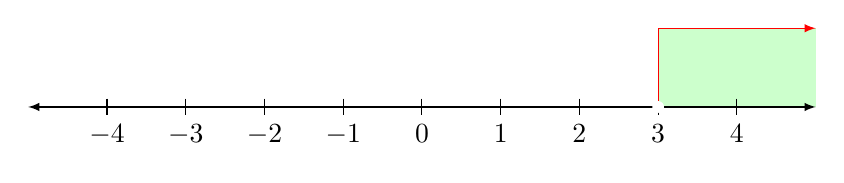
\begin{tikzpicture}
        \fill[green!20](5,0)rectangle(3,1);
        \draw[latex-latex] (-5,0) -- (5,0) ;
        \foreach \x in {-4,-3,-2,-1,0,1,2,3,4} \draw[shift={(\x,0)},color=black] (0pt,3pt) -- (0pt,-3pt) node[below] {$\x$};
        %\node[circle,fill=white,inner sep=1.5pt](a)at(0,0){};
        \node[circle,fill=white,inner sep=1.5pt](b)at(3,0){};
        %\node[circle,fill=black,inner sep=1.5pt](c)at(-3,0){};
        \draw[-latex,red](b)--++(0,1)--++(2,0);
    \end{tikzpicture}
    \caption{\color{blue}{Graphical representation of the domain of $\log_2(x-3)$}}
    \end{figure}
    
\vspace{1in}

    
    \begin{figure}[htbp]
        \centering
        \includegraphics[width=0.6\textwidth]{log1_10}
        \caption{\color{blue}{Graph of the function $\log_2(x-3)$ showing the asymptote $x=3$ and the domain $x>3$}}
        %\label{fig:myimage}
    \end{figure}
}
\begin{tcolorbox}[title=Answer, colback=blue!10!white, colframe=blue!75!black]
Domain in Interval Notation: $x\in (3,\infty)$\\
Domain in Set-builder notation: $\{ x \in \mathbb{R} \mid x>3 \}$\\
Asymptote: $x=3$
\end{tcolorbox}

\newpage    
\item $y=\ln(x^2-16)$

{\color{blue}
The argument of the lo is $x^2-16$. 
\begin{itemize}
    \item Factor the argument
    \item Find the zeros of the argument
    \item Identify the regions where each factor is positive/negative
    \item Identify the regions where the argument is positive/negative
\end{itemize}

 Factor the argument then find the zeros:
    \begin{align*}
        x^2-16&=0\\
        (x-4)(x+4)&=0\\
        x-4=0,\quad& x+4=0\\
        x=4,\quad& x=-4
    \end{align*}

    Setup a table showing the sign of each factor then the overall sign of the argument.
    \begin{align*}
        x-4>0&\Rightarrow x>4\\
        x+4>0&\Rightarrow x>-4
    \end{align*}

From the table we see that the argument is positive to the right of $x=4$ and to the left of $x=-4$. We can also see the asymptotes at $x=\pm 4$
\vspace{1in}

 \begin{figure}[!h]
    \centering    
\begin{tikzpicture}
\tkzTabInit[lgt=4,espcl=2,deltacl=0]
  { /.8, $x-4$ /.8, $x+4$ /.8, $(x-4)(x+4)$ /.8}
  {,$-4$,$4$,} % four main references
\tkzTabLine {,-,t,-,z,+,} % seven denotations
\tkzTabLine {,-,z,+,t,+,}
\tkzTabLine {,+,z,-,z,+,}
\end{tikzpicture}
\caption{}
\end{figure}

 
\newpage
\begin{figure}[!h]
    \centering
    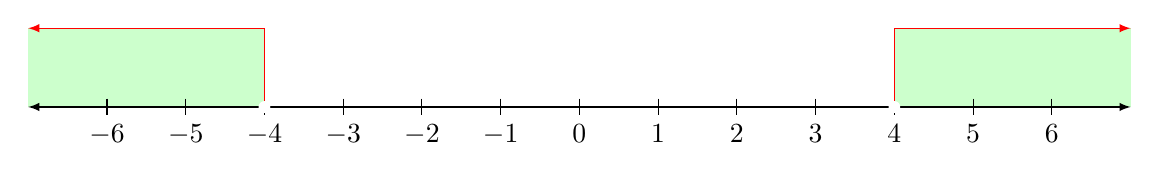
\begin{tikzpicture}
        \fill[green!20](7,0)rectangle(4,1);
        \fill[green!20](-7,0)rectangle(-4,1);
        \draw[latex-latex] (-7,0) -- (7,0) ;
        \foreach \x in {-6,-5,-4,-3,-2,-1,0,1,2,3,4,5,6} \draw[shift={(\x,0)},color=black] (0pt,3pt) -- (0pt,-3pt) node[below] {$\x$};
        \node[circle,fill=white,inner sep=1.5pt](a)at(-4,0){};
        \node[circle,fill=white,inner sep=1.5pt](b)at(4,0){};
        %\node[circle,fill=black,inner sep=1.5pt](c)at(-3,0){};
        \draw[-latex,red](a)--++(0,1)--++(-3,0);
        \draw[-latex,red](b)--++(0,1)--++(3,0);
    \end{tikzpicture}
    \caption{\color{blue}{Graphical representation of the domain of $\ln(x^2-4)$}}
    \end{figure}

\vspace{1in}
We can also identify the domain and asymptotes by plotting the function as showin below.  

    \begin{figure}[htbp]
        \centering
        \includegraphics[width=0.6\textwidth]{log1_11}
        \caption{\color{blue}{Graph of the function $\ln(x^2-16)$ showing the asymptotes $x=\pm 4$ and the domain $x\in (-\infty,-4)\cup (4,\infty)$}}
        %\label{fig:myimage}
    \end{figure}
 }   

\begin{tcolorbox}[title=Answer, colback=blue!10!white, colframe=blue!75!black]
Domain in Interval Notation: $x\in (-\infty,-4)\cup (4,\infty)$\\
Domain in Set-builder notation: $\{ x \in \mathbb{R} \mid x\ne \pm4 \}$\\
Asymptotes: $x=\pm 4$  
\end{tcolorbox}
 
\newpage
\item $y=\log(x^2+5x+6)$
    {\color{blue}
    \begin{align*}
        x^2+5x+6&=0\\
        (x+2)(x+3)&=0\\
        x+2=0,\quad&x+3=0\\
        x=-2,\quad& x=-3
    \end{align*}


    Setup a table showing the sign of each factor then the overall sign of the argument looking for regions of positive sign.
    \begin{align*}
        x+2>0&\Rightarrow x>-2\\
        x+3>0&\Rightarrow x>-3
    \end{align*}

 \begin{figure}[!h]
    \centering    
\begin{tikzpicture}
\tkzTabInit[lgt=4,espcl=2,deltacl=0]
  { /.8, $x+2$ /.8, $x+3$ /.8, $(x+2)(x+3)$ /.8}
  {,$-3$,$-2$,} % four main references
\tkzTabLine {,-,t,-,z,+,} % seven denotations
\tkzTabLine {,-,z,+,t,+,}
\tkzTabLine {,+,z,-,z,+,}
\end{tikzpicture}
%\caption{}
\end{figure}

\begin{figure}[!h]
    \centering
    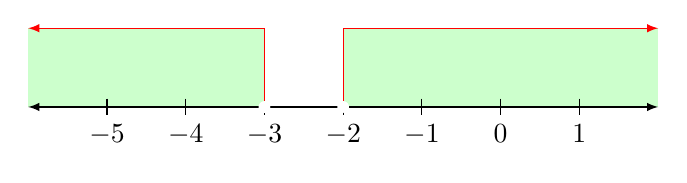
\begin{tikzpicture}
        \fill[green!20](-6,0)rectangle(-3,1);
        \fill[green!20](-2,0)rectangle(2,1);
        \draw[latex-latex] (-6,0) -- (2,0) ;
        \foreach \x in {-5,-4,-3,-2,-1,0,1} \draw[shift={(\x,0)},color=black] (0pt,3pt) -- (0pt,-3pt) node[below] {$\x$};
        \node[circle,fill=white,inner sep=1.5pt](a)at(-3,0){};
        \node[circle,fill=white,inner sep=1.5pt](b)at(-2,0){};
        %\node[circle,fill=black,inner sep=1.5pt](c)at(-3,0){};
        \draw[-latex,red](a)--++(0,1)--++(-3,0);
        \draw[-latex,red](b)--++(0,1)--++(4,0);
    \end{tikzpicture}
    \caption{\color{blue}{Graphical representation of the domain of $\log(x^2+5x+6)$}}
    \end{figure}
\newpage
    \begin{figure}[htbp]
        \centering
        \includegraphics[width=0.6\textwidth]{log1_12}
        \caption{\color{blue}{Graph of the function $\log(x^2+5x+6)$ showing the asymptotes $x=-3$ and $x=-2$ and the domain $x\in (-\infty,-3)\cup (-2,\infty)$}}
        %\label{fig:myimage}
    \end{figure}

    }

\begin{tcolorbox}[title=Domain and Asymptotes, colback=blue!10!white, colframe=blue!75!black]
Domain: Interval Notation: $x\in (-\infty,-3)\cup (-2,\infty)$\\
Domain: Set-builder notation: $\{ x \in \mathbb{R} \mid x\ne -3,-2 \}$\\
Asymptotes: $x=-3, x=-2$  
\end{tcolorbox}




\newpage
\item $y=\log\left(\sqrt{2x-1}+2\right)$
    {\color{blue}

A close look at the argument of log indicates that it cannot be zero or negative, only positive. So we just need to focus on the quantity under the square root and ensure that it's not negative.

    \begin{align*}
        2x-1&\ge 0\\
        2x&\ge 1\\
        x&\ge \frac{1}{2}
    \end{align*}

For $x\ge\frac{1}{2}$, the argument of the log is positive and real.





\begin{figure}[!h]
    \centering
    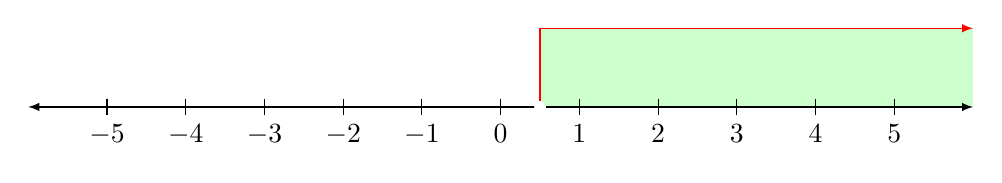
\begin{tikzpicture}
        \fill[green!20](0.5,0)rectangle(6,1);
        \draw[latex-latex] (-6,0) -- (6,0) ;
        \foreach \x in {-5,-4,-3,-2,-1,0,1,2,3,4,5} \draw[shift={(\x,0)},color=black] (0pt,3pt) -- (0pt,-3pt) node[below] {$\x$};
        \node[circle,fill=white,inner sep=1.5pt](a)at(0.5,0){};
        %\node[circle,fill=white,inner sep=1.5pt](b)at(-2,0){};
        %\node[circle,fill=black,inner sep=1.5pt](c)at(-3,0){};
        \draw[-latex,red](a)--++(0,1)--++(5.5,0);
        %\draw[-latex,red](b)--++(0,1)--++(4,0);
    \end{tikzpicture}
    \caption{\color{blue}{Graphical representation of the domain of $\log\left(\sqrt{2x-1}+2\right)$}}
    \end{figure}


    \begin{figure}[htbp]
        \centering
        \includegraphics[width=0.6\textwidth]{log1_13}
        \caption{\color{blue}{Graph of the function $\log\left(\sqrt{2x-1}+2\right)$ the domain $x\in [\frac{1}{2},\infty)$}. We can see that there we don't have an asymptote at $x=\frac{1}{2}$ - the value of the function there is finite.}
        %\label{fig:myimage}
    \end{figure}

    }
  \begin{tcolorbox}[title=Domain and Asymptotes, colback=blue!10!white, colframe=blue!75!black]
Domain: Interval Notation: $x\in [\frac{1}{2},\infty)$\\
Domain: Set-builder notation: $\{ x \in \mathbb{R} \mid x\ge \frac{1}{2}\}$\\
Asymptotes: None 
\end{tcolorbox}  
    
\newpage
\item $y=\ln\left(\dfrac{2-x}{\sqrt{x+4}}\right)$
{\color{blue}

The denominator of the argument should be real and non zero. The numerator should be strictly positive. Put these together 

    \begin{align*}
        x+4>0 &\quad\text{and}\quad 2-x>0\\
        x> -4 &\quad\text{and}\quad x < 2
    \end{align*}

Put these results in a table to get region 

 \begin{figure}[!h]
    \centering    
\begin{tikzpicture}
\tkzTabInit[lgt=4,espcl=2,deltacl=0]
  { /.8, $2-x$ /.8, $x+4$ /.8, $\frac{2-x}{\sqrt{x+4}}$ /.8}
  {,$-4$,$2$,} % four main references
\tkzTabLine {,+,t,+,z,-,} % seven denotations
\tkzTabLine {,$\nexists$,z,+,t,+,}
\tkzTabLine {,$\nexists$,t,+,t,-,}
\end{tikzpicture}
\caption{The tables shows the domain of the function is $-4<x<2$}
\end{figure}



\vspace{1in}
The domain can also be represented graphically as shown below:
\vspace{0.5in}
\begin{figure}[!h]
    \centering
    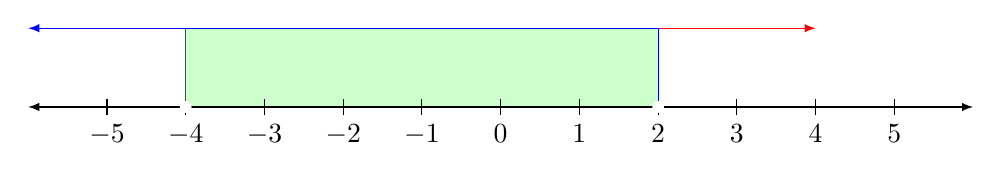
\begin{tikzpicture}
        \fill[green!20](-4,0)rectangle(2,1);

        \draw[latex-latex] (-6,0) -- (6,0) ;
        \foreach \x in {-5,-4,-3,-2,-1,0,1,2,3,4,5} \draw[shift={(\x,0)},color=black] (0pt,3pt) -- (0pt,-3pt) node[below] {$\x$};
        \node[circle,fill=white,inner sep=1.5pt](a)at(-4,0){};
        \node[circle,fill=white,inner sep=1.5pt](b)at(2,0){};
        %\node[circle,fill=black,inner sep=1.5pt](c)at(-3,0){};
        \draw[-latex,red](a)--++(0,1)--++(8,0);
        \draw[-latex,blue](b)--++(0,1)--++(-8,0);
    \end{tikzpicture}
    \caption{\color{blue}{Graphical representation of the domain of $y=\ln\left(\dfrac{2-x}{\sqrt{x+4}}\right)$}}
    \end{figure}

\newpage
    \begin{figure}[htbp]
        \centering
        \includegraphics[width=0.6\textwidth]{log1_14}
        \caption{\color{blue}{Graph of the function $y=\ln\left(\dfrac{2-x}{\sqrt{x+4}}\right)$ showing the domain $x\in (-4,2)$. We also have two asymptotes at $x=-4$ and $x=2$}}
        %\label{fig:myimage}
    \end{figure}

\vspace{1in}
\begin{tcolorbox}[title=Domain and Asymptotes, colback=blue!10!white, colframe=blue!75!black]
Domain: Interval Notation: $x\in (-4,2)$\\
Domain: Set-builder notation: $\{ x \in \mathbb{R} \mid -4<x<2\}$\\
Asymptotes: $x=-4$ and $x=2$. 
\end{tcolorbox}


    }






\newpage
\item $y=\log_2(x^2+1)-3x$
{\color{blue}

The argument of the log should be strictly positive.  But the argument $x^2+1$ is always positive (this is a parabola $x^2$ that is shifted up 1 unit so it does not touch or cross the $x-$axis). So, there are no restrictions on $x$. The second term, $-3x$,  is a monomial and its domain is $\mathbb{R}$. 

Thus the domain of the function is $\mathbb{R}$ and it has no vertical asymptotes. This can be verified from the graph below. 

\vspace{0.5in}
    \begin{figure}[htbp]
        \centering
        \includegraphics[width=0.9\textwidth]{log1_15}
        \caption{\color{blue}{Graph of the function $y=\log_2(x^2+1)-3x$ showing the domain $x\in (-\infty,\infty)$. This function does not have any asymptotes.}}
        %\label{fig:myimage}
    \end{figure}

\vspace{0.5in}
\begin{tcolorbox}[title=Domain and Asymptotes, colback=blue!10!white, colframe=blue!75!black]
Domain: Interval Notation: $x\in (-\infty,\infty)$\\
Domain: Set-builder notation: $\{ x \in \mathbb{R}\}$\\
Asymptotes: None 
\end{tcolorbox}


}



\newpage
\item $y=\log(x+3)^2$
{\color{blue}

The argument of the log, $(x+3)^2$ will never be negative (for real values of $x$) but can be zero at $x=-3$.  Thus, the domain of the function is the real numbers excluding -3, where we have a vertical asymptote.
\vspace{0.5in}
    \begin{figure}[htbp]
        \centering
        \includegraphics[width=0.6\textwidth]{log1_16}
        \caption{\color{blue}{Graph of the function $y=\log(x+3)^2$ showing the domain $x\in (-\infty,-3)\cup(-3,\infty)$. We also have an asymptote at $x=-3$}}
        %\label{fig:myimage}
    \end{figure}

\vspace{0.5in}
\begin{tcolorbox}[title=Domain and Asymptotes, colback=blue!10!white, colframe=blue!75!black]
Domain: Interval Notation: $x\in (-\infty,-3)\cup(-3,\infty)$\\
Domain: Set-builder notation: $\{ x \in \mathbb{R} \mid c\ne 3\}$\\
Asymptotes: $x=-3$ 
\end{tcolorbox}


}


\newpage
\item $y=\log\left(\dfrac{x-3}{x+2}\right)$
{\color{blue}

The domain of the function depends on the sign and values of the ratio. First find the zeros by setting each term to zero

    \begin{align*}
        x+3=0 &\quad\text{and}\quad x+2=0\\
        x= -3 &\quad\text{and}\quad x= -2
    \end{align*}

Find the regions where each factor is positive (otherwise it's negative)
    \begin{align*}
        x-3>0 &\quad\text{and}\quad x+2>0\\
        x> -3 &\quad\text{and}\quad x > -2
    \end{align*}

Setup a table to get the overall signs of the quotient:

 \begin{figure}[!h]
    \centering    
\begin{tikzpicture}
\tkzTabInit[lgt=4,espcl=2,deltacl=0]
  { /.8, $x-3$ /.8, $x+2$ /.8, $\frac{x-3}{x+2}$ /.8}
  {,$-2$,$3$,} % four main references
\tkzTabLine {,-,z,+,t,+,} % seven denotations
\tkzTabLine {,-,t,-,z,+,}
\tkzTabLine {,+,t,-,t,+,}
\end{tikzpicture}
\caption{The tables shows the domain of the function is $x<-2$ and $x>3$}
\end{figure}



\vspace{0.5in}
The domain can also be represented graphically as shown below:
\vspace{0.5in}
\begin{figure}[!h]
    \centering
    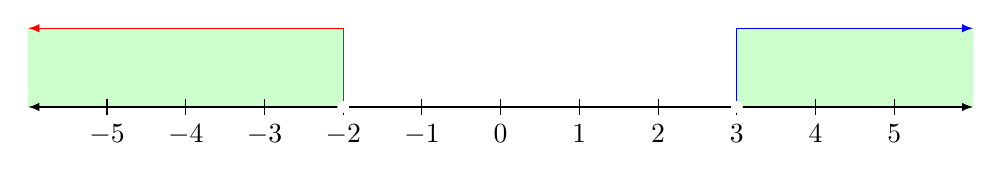
\begin{tikzpicture}
        \fill[green!20](-2,0)rectangle(-6,1);
        \fill[green!20](3,0)rectangle(6,1);
        \draw[latex-latex] (-6,0) -- (6,0) ;
        \foreach \x in {-5,-4,-3,-2,-1,0,1,2,3,4,5} \draw[shift={(\x,0)},color=black] (0pt,3pt) -- (0pt,-3pt) node[below] {$\x$};
        \node[circle,fill=white,inner sep=1.5pt](a)at(-2,0){};
        \node[circle,fill=white,inner sep=1.5pt](b)at(3,0){};
        %\node[circle,fill=black,inner sep=1.5pt](c)at(-3,0){};
        \draw[-latex,red](a)--++(0,1)--++(-4,0);
        \draw[-latex,blue](b)--++(0,1)--++(3,0);
    \end{tikzpicture}
    \caption{\color{blue}{Graphical representation of the domain of $y=\log\left(\dfrac{x-3}{x+2}\right)$}}
    \end{figure}

\newpage
    \begin{figure}[htbp]
        \centering
        \includegraphics[width=0.6\textwidth]{log1_17}
        \caption{\color{blue}{Graph of the function $y=\log\left(\dfrac{x-3}{x+2}\right)$ showing the domain $x\in (-\infty,-2)\cup(3,\infty)$. We also have two asymptotes at $x=-2$ and $x=3$}}
        %\label{fig:myimage}
    \end{figure}

\vspace{1in}
\begin{tcolorbox}[title=Domain and Asymptotes, colback=blue!10!white, colframe=blue!75!black]
Domain: Interval notation: $x\in (-\infty,-2)\cup(3,\infty)$\\
Domain: Set-builder notation: $\{ x \in \mathbb{R} \mid x<-2 \text{ and } x>3\}$\\
Asymptotes: $x=-2$ and $x=3$. 
\end{tcolorbox}

}



\newpage
\item $y=\ln\left(\sqrt{x-2}-1\right)$
{\color{blue}

The argument of the log should be strictly positive.  But the argument $x^2+1$ is always positive (this is a parabola $x^2$ that is shifted up 1 unit so it does not touch or cross the $x-$axis). So, there are no restrictions on $x$. The second term, $-3x$,  is a monomial and its domain is $\mathbb{R}$. 

Thus the domain of the function is $\mathbb{R}$ and it has no vertical asymptotes. This can be verified for the graph below. 

    \begin{align*}
        x+4>0 &\quad\text{and}\quad 2-x>0\\
        x> -4 &\quad\text{and}\quad x < 2
    \end{align*}

Put these results in a table to get region 

 \begin{figure}[!h]
    \centering    
\begin{tikzpicture}
\tkzTabInit[lgt=4,espcl=2,deltacl=0]
  { /.8, $x-2$ /.8, $\sqrt{x-2}-1$ /.8, overlap /.8}
  {,$2$,$3$,} % four main references
\tkzTabLine {,$\nexists$,z,+,t,+,} % seven denotations
\tkzTabLine {,$\nexists$,t,$\nexists$,z,+,}
\tkzTabLine {,$\nexists$,t,$\nexists$,t,+,}
\end{tikzpicture}
\caption{The tables shows the domain of the function is $x>3$}
\end{figure}



\vspace{1in}
The domain can also be represented graphically as shown below:
\vspace{0.5in}
\begin{figure}[!h]
    \centering
    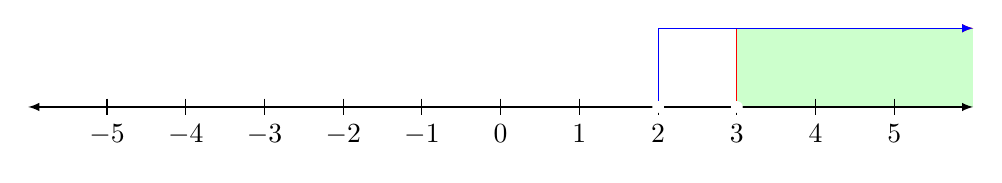
\begin{tikzpicture}
        \fill[green!20](6,0)rectangle(3,1);

        \draw[latex-latex] (-6,0) -- (6,0) ;
        \foreach \x in {-5,-4,-3,-2,-1,0,1,2,3,4,5} \draw[shift={(\x,0)},color=black] (0pt,3pt) -- (0pt,-3pt) node[below] {$\x$};
        \node[circle,fill=white,inner sep=1.5pt](a)at(3,0){};
        \node[circle,fill=white,inner sep=1.5pt](b)at(2,0){};
        %\node[circle,fill=black,inner sep=1.5pt](c)at(-3,0){};
        \draw[-latex,red](a)--++(0,1)--++(3,0);
        \draw[-latex,blue](b)--++(0,1)--++(4,0);
    \end{tikzpicture}
    \caption{\color{blue}{Graphical representation of the domain of $y=\ln\left(\dfrac{2-x}{\sqrt{x+4}}\right)$}}
    \end{figure}

\newpage
    \begin{figure}[htbp]
        \centering
        \includegraphics[width=0.6\textwidth]{log1_18}
        \caption{\color{blue}{Graph of the function $y=\ln\left(\sqrt{x-2}-1\right)$ showing the domain $x\in (3,\infty)$. We also have an asymptote at $x=3$}}
        %\label{fig:myimage}
    \end{figure}

\vspace{1in}
\begin{tcolorbox}[title=Domain and Asymptotes, colback=blue!10!white, colframe=blue!75!black]
Domain: Interval Notation: $x\in (3,\infty)$\\
Domain: Set-builder notation: $\{ x \in \mathbb{R} \mid x>3\}$\\
Asymptotes: $x=3$. 
\end{tcolorbox}
}

\end{enumerate}

% \section*{Plot Using Transformations}
\chead{Plot Using Transformations}
\begin{tcolorbox}[title=Hint, colback=teal!10!white, colframe=teal!75!black]
The table below shows how a function $f(x)$ is transformed under different conditions. The order of transformations is important. Here is the suggested order of transformations
\begin{itemize}
    \item Horizontal translation or shift: $f(x)\rightarrow f(x\pm h)$
    \item Horizontal and vertical stretch (or shrink): $f(x)\rightarrow f(ax) \text{ or }af(x)$.
    \item Reflections about the $x-$ and $y-$axes: $f(x)\rightarrow f(-x) \text{ or } -f(x)$.
    \item Vertical translation or shift: $f(x)\rightarrow f(x) \pm k$
\end{itemize}
\vspace{0.5in}
When applying the transformations outlined in the table, it's helpful to select three or more points from the original function and track how each point changes (as illustrated in the last column on the table). This method helps to visualize the transformation accurately. Remember that vertical asymptotes will only be affected by horizontal transformations.

\vspace{0.5in}
This approach was demonstrated in our solved problems, where we also indicated the direction of each translation.
\end{tcolorbox}
\newpage
% %%%%%%%%%%%%%%%%%%%%%%%%%%%%%%%%%%%%%%%%%%%%%%%%%%%%%%%%%%%%%%%%%%%%%%%%%%%%%%%
% %%%
% %%%                     PLOT THE FOLLOWING LOGARITHMS
% %%%
% %%%%%%%%%%%%%%%%%%%%%%%%%%%%%%%%%%%%%%%%%%%%%%%%%%%%%%%%%%%%%%%%%%%%%%%%%%%%%%%
% \subsection*{Graph Using Transformations. Identify The Domain and The Vertical Asymptote(s)}
% \begin{tcolorbox}[title=Note, colback=blue!10!white, colframe=blue!75!black]
% tt
% \end{tcolorbox}

\noindent These are the cases in which a function $f(x)$ gets transformed. Assume that  $h$, $k$, and $a$ are positive real numbers. This is also the order of transformations in a multi-transformation steps problem. 
\begin{table}[h]
\centering
\renewcommand{\arraystretch}{2}
\begin{tabular}{|>{\bfseries}p{0.35\textwidth}|p{0.35\textwidth}|p{0.25\textwidth}|}
\hline
\rowcolor{blue!75!black}\color{white}\textbf{Transformation Type} & \color{white}\textbf{Effect on the Graph of \boldmath$f$} & \color{white}\textbf{How Points Change on \boldmath$f$} \\
\hline
\textbf{Horizontal translation (shift)} & & \\
$y = f(x - h)$ & Shift graph right $h$ units &  $(x, y)\rightarrow(x + h, y)$ \\
$y = f(x + h)$ & Shift graph left $h$ units &  $(x, y)\rightarrow(x - h, y)$ \\
\hline
\textbf{Horizontal stretch/shrink} & $a > 1:$Horizontal shrink & \\
$y = f(a \cdot x)$ & $0 < a < 1:$Horizontal stretch &  $(x, y)\rightarrow\left(\frac{x}{a}, y\right)$ \\
& Stretch/shrink graph horizontally by a factor of $\frac{1}{a}$ & \\
\hline
\textbf{Vertical stretch/shrink} & $a > 1:$Vertical stretch  & \\
$y = a[f(x)]$ & $0 < a < 1:$Vertical shrink &  $(x, y)\rightarrow(x, ay)$ \\
& Stretch/shrink graph vertically by a factor of $a$ & \\
\hline
\textbf{Reflection} & & \\
$y = -f(x)$ & Reflect  graph across the $x$-axis &  $(x, y)\rightarrow(x, -y)$ \\
$y = f(-x)$ & Reflect  graph across the $y$-axis &  $(x, y)\rightarrow(-x, y)$ \\
\hline
\textbf{Vertical translation (shift)} & & \\
$y = f(x) + k$ & Shift graph up $k$ units &  $(x, y)\rightarrow(x, y + k)$ \\
$y = f(x) - k$ & Shift graph down $k$ units &  $(x, y)\rightarrow(x, y - k)$ \\
\hline
\end{tabular}
\end{table}







\newpage
\begin{enumerate}[resume]
    \item $f(x)=\log_2(x-3)$
    {\color{blue}
    \begin{figure}[htbp]
        \centering
        \includegraphics[width=0.9\textwidth]{log1_19}
        \caption{Shift $f(x)=\log_2(x)$ to the right 3 units: $(x,y)\rightarrow(x+3, y)$. Also shift the asymptote from $x=0$ to $x=3$}
        %\label{fig:myimage}
    \end{figure}
}
% -----------------------------------------------------------------------------------
    
\newpage 
\item $f(x)=\log_3(1+x)+2$
    {\color{blue}
        \begin{figure}[htbp]
        \centering
        \includegraphics[width=0.8\textwidth]{log1_20}
        \caption{$1^\text{st}$ transformation: $f(x)\rightarrow f(x+1);\log_3(x)\rightarrow\log_3(1+x)$. \\Shift $f(x)$ to the left 1 unit: $(x,y)\rightarrow(x-1,y)$. Move the asymptote $x=0$ to $x=-1$}
        %\label{fig:myimage}
    \end{figure}

        \begin{figure}[htbp]
        \centering
        \includegraphics[width=0.8\textwidth]{log1_21}
        \caption{$2^\text{nd}$ transformation: $f(x+1)\rightarrow f(x+1)+2;\log_3(x+1)\rightarrow\log_3(1+x)+2$. \\ Shift $f(x+1)$ up 2 units: $(x,y)\rightarrow(x,y+2)$. The asymptote stays the same.}
        %\label{fig:myimage}
    \end{figure}

    
    }
    
% -----------------------------------------------------------------------------------
    
\newpage    
\item $f(x)=4-2\ln(x+2)$
    {\color{blue}
        \begin{figure}[htbp]
        \centering
        \includegraphics[width=0.8\textwidth]{log1_22}
        \caption{$1^\text{st}$ transformation: $f(x)\rightarrow f(x+2);\ln(x)\rightarrow\ln(x+2)$. \\Shift $f(x)$ to the left 2 unit: $(x,y)\rightarrow(x-2,y)$. Move the asymptote $x=0$ to $x=-2$}
        %\label{fig:myimage}
    \end{figure}

        \begin{figure}[htbp]
        \centering
        \includegraphics[width=0.8\textwidth]{log1_23}
        \caption{$2^\text{nd}$ transformation: $f(x+2)\rightarrow 2f(x+2);\ln(x+2)\rightarrow 2\ln(x+2)$. \\ Stretch $f(x+2)$ vertically by 2: $(x,y)\rightarrow(x,2y)$. The asymptote stays the same.}
        %\label{fig:myimage}
    \end{figure}
            \begin{figure}[htbp]
        \centering
        \includegraphics[width=0.8\textwidth]{log1_24}
        \caption{$3^\text{rd}$ transformation: $2f(x+2)\rightarrow -2f(x+2);2\ln(x+2)\rightarrow -2\ln(x+2)$. \\ Reflect $2f(x+1)$ about the $x-$axis: $(x,y)\rightarrow(x,-y)$. The asymptote stays the same.}
        %\label{fig:myimage}
    \end{figure}

        \begin{figure}[htbp]
        \centering
        \includegraphics[width=0.8\textwidth]{log1_25}
        \caption{$4^\text{th}$ transformation: $-2f(x+2)\rightarrow -2f(x+2)+4;-2\ln(x+2)\rightarrow -2\ln(x+2)+4$. \\ Shift $-2f(x+1)$ up 4 units: $(x,y)\rightarrow(x,y+4)$. The asymptote stays the same.}
        %\label{fig:myimage}
    \end{figure}
    }

% -----------------------------------------------------------------------------------
    
\newpage 
\item $f(x)=4-\log(4-x)$
    {\color{blue}
        \begin{figure}[htbp]
        \centering
        \includegraphics[width=0.8\textwidth]{log1_26}
        \caption{$1^\text{st}$ transformation: $f(x)\rightarrow f(x+4);\log(x)\rightarrow\log(x+4)$. \\Shift $f(x)$ to the left 4 unit: $(x,y)\rightarrow(x-4,y)$. Move the asymptote $x=0$ to $x=-4$}
        %\label{fig:myimage}
    \end{figure}

        \begin{figure}[htbp]
        \centering
        \includegraphics[width=0.8\textwidth]{log1_27}
        \caption{$2^\text{nd}$ transformation: $f(x+4)\rightarrow f(-x+4);\log(x+4)\rightarrow\log(-x+4)$. \\ Reflect $f(x+4)$ about the $y-$axis: $(x,y)\rightarrow(-x,y)$. Move the asymptote $x=-4$ to $x=4$}
        %\label{fig:myimage}
    \end{figure}
            \begin{figure}[htbp]
        \centering
        \includegraphics[width=0.8\textwidth]{log1_28}
        \caption{$3^\text{rd}$ transformation: $f(-x+4)\rightarrow -f(-x+4);\log(-x+4)\rightarrow -\log(-x+4)$. \\ Reflect $f(-x+4)$ about the $x-$axis: $(x,y)\rightarrow(x,-y)$. The asymptote stays the same.}
        %\label{fig:myimage}
    \end{figure}

        \begin{figure}[htbp]
        \centering
        \includegraphics[width=0.8\textwidth]{log1_29}
        \caption{$4^\text{th}$ transformation: $-f(-x+4)\rightarrow -f(-x+4)+4;-\log(-x+4)\rightarrow -\log(-x+4)+4$. \\ Shift $-f(-x+4)$ up 4 units: $(x,y)\rightarrow(x,y+4)$. The asymptote stays the same.}
        %\label{fig:myimage}
    \end{figure}
    
    }

\newpage
\item $y=3\log_2(2x+1)-2$
    {\color{blue}
        \begin{figure}[htbp]
        \centering
        \includegraphics[width=0.7\textwidth]{log1_30}
        \caption{$1^\text{st}$ transformation: $f(x)\rightarrow f(x+1);\log_2(x)\rightarrow\log_2(x+1)$. \\Shift $f(x)$ to the left 1 unit: $(x,y)\rightarrow(x-1,y)$. Move the asymptote $x=0$ to $x=-1$}
        %\label{fig:myimage}
    \end{figure}

        \begin{figure}[htbp]
        \centering
        \includegraphics[width=0.7\textwidth]{log1_31}
        \caption{$2^\text{st}$ transformation: $f(x+1)\rightarrow f(2x+1);\log_2(x+1)\rightarrow\log_2(2x+1)$. \\ Shrink $f(x+1)$ horizontally by a factor of 2: $(x,y)\rightarrow(x/2,y)$. Move the asymptote $x=-1$ to $x=-0.5$}
        %\label{fig:myimage}
    \end{figure}
            \begin{figure}[htbp]
        \centering
        \includegraphics[width=0.7\textwidth]{log1_32}
        \caption{$3^\text{rd}$ transformation: $f(2x+1)\rightarrow 3f(2x+1);\log_2(2x+1)\rightarrow 3\log_2(2x+1)$. \\ Stretch $f(2x+1)$ vertically by a factor of 3: $(x,y)\rightarrow(x,3y)$. The asymptote stays the same.}
        %\label{fig:myimage}
    \end{figure}

        \begin{figure}[htbp]
        \centering
        \includegraphics[width=0.7\textwidth]{log1_33}
        \caption{$4^\text{th}$ transformation: $3f(2x+1)\rightarrow 3f(2x+1)-2;3\log_2(2x+1)\rightarrow 3\log_2(2x+1)-1$. \\ Shift $3f(2x+1)$ vertically down by 2 units: $(x,y)\rightarrow(x,y-2)$. The asymptote stays the same.}
        %\label{fig:myimage}
    \end{figure}
    
}
\end{enumerate}
% \chead{Expand Completely}

\newpage
%%%%%%%%%%%%%%%%%%%%%%%%%%%%%%%%%%%%%%%%%%%%%%%%%%%%%%%%%%%%%%%%%%%%%%%%%%%%%%%
%%%
%%%                     EXPAND COMPLETELY
%%%
%%%%%%%%%%%%%%%%%%%%%%%%%%%%%%%%%%%%%%%%%%%%%%%%%%%%%%%%%%%%%%%%%%%%%%%%%%%%%%%
\noindent\subsection*{Expand Completely}
\begin{tcolorbox}[title=Note, colback=blue!10!white, colframe=blue!75!black]
Use the properties to write in simplest form. In particular, use the power, product and quotient rules. 
\end{tcolorbox}
\vspace{0.6cm}
\begin{enumerate}[resume]
    \item $\log_4(x^3)$:
    
    {\color{blue}
        \begin{align*}
        \Aboxed{\log_4(x^3)=3\log_4(x)\makebox[5cm]{\dotfill}\textit{Power Rule}}
    \end{align*}
    }

    
    
    \item $\log_7(49x)$:
    
    {\color{blue}
    \begin{align*}
        \log_7(49x)&=\log_7(49)+\log_7(x)\makebox[5cm]{\dotfill}\textit{Product Rule}\\
        &=\log_7(7^2)+\log_7(x)\\
        \Aboxed{&=2+\log_2(x)\makebox[5cm]{\dotfill}\textit{Inverse Property}}
    \end{align*}
    }


    
    \item $\log_2(5xy)$
    
    {\color{blue}
    \begin{align*}
        \log_2(5xy)&=\log_2(5(xy))\\
        &=\log_2(5)+\log_2(xy)\makebox[7cm]{\dotfill}\textit{Product Rule}\\
        \Aboxed{&=\log_2(5)+\log_2(x)+\log_2(y)\makebox[5cm]{\dotfill}\textit{Product Rule}}
    \end{align*}
    }
    



    \item  $\log_{10}(x^2y^3)$
    
    {\color{blue}
    \begin{align*}
        \log_{10}(x^2y^3)&=\log(x^2+y^2)\makebox[5cm]{\dotfill}\log_{10}u=\log u\\
        &=\log(x^2)+\log(y^3)\makebox[5cm]{\dotfill}\textit{Product Rule}\\
        \Aboxed{&=2\log(x)+3\log(y)\makebox[5cm]{\dotfill}\textit{Power Rule}}
    \end{align*}
    }


    \item  $\log_2\left(\dfrac{x^3y^2}{z^4}\right)$
    
    {\color{blue}
    \begin{align*}
        \log_2\left(\dfrac{x^3y^2}{z^4}\right)&=\log_2(x^3y^2)-\log_2(z^4)\makebox[4cm]{\dotfill}\textit{Quotient Rule}\\
        &=\log_2(x^3)+\log_2(y^2)-\log_2(z^4)\makebox[3cm]{\dotfill}\textit{Product Rule}\\
        \Aboxed{&=3\log_2(x)+2\log_2(y)-4\log_2(z)\makebox[3cm]{\dotfill}\textit{Power Rule}}
    \end{align*}
    }


    \item $\log\left(\dfrac{\sqrt{f^2-3}}{1000}\right)$
    
    {\color{blue}
        \begin{align*}
            \log\left(\dfrac{\sqrt{f^2-3}}{1000}\right)&=\log\left(\dfrac{(f^2-3)^{1/2}}{10^3}\right)\makebox[4cm]{\dotfill}\sqrt{a}=a^{1/2}\\
            &=\log\left(f^2-3\right)^{1/2}-\log\left({10^3}\right)\makebox[2cm]{\dotfill}\textit{Quotient Rule}\\
            &=\dfrac{1}{2}\log\left(f^2-3\right)-3\makebox[2cm]{\dotfill}\textit{Power and Identity Rules}\\
            &=\dfrac{1}{2}\left(\log(f-\sqrt{3})(f+\sqrt{3})\right)-3\makebox[1cm]{\dotfill}a^2-b^2=(a-b)(a+b)\\
            &=\dfrac{1}{2}\left(\log(f-\sqrt{3})+\log(f+\sqrt{3})\right)-3\makebox[1cm]{\dotfill}\textit{Product Rule}\\
            \Aboxed{&=\dfrac{1}{2}\log(f-\sqrt{3}) +\dfrac{1}{2}\log(f+\sqrt{3})-3}\\
        \end{align*}
    }
    


    \item  $\log_3\left(\dfrac{x^2\sqrt[3]{y}}{(z+1)^4}\right)$
    
    {\color{blue}
    \begin{align*}
        \log_3\left(\dfrac{x^2\sqrt[3]{y}}{(z+1)^4}\right)&=\log_3(x^2\sqrt[3]{y})-\log_3(z^4)\makebox[3cm]{\dotfill}\textit{Quotient Rule}\\
        &=\log_3(x^2)+\log_3(y^{1/3})-\log_2((z+1)^4)\makebox[2cm]{\dotfill}\textit{Product Rule}\\
        \Aboxed{&=2\log_3(x)+\dfrac{1}{3}\log_3(y)-4\log_2(z+1)\makebox[2cm]{\dotfill}\textit{Power Rule}}
    \end{align*}
    }

    
    \item  $\log_7\left(\dfrac{\sqrt{x}}{y^2z}\right)$
    
        {\color{blue}
    \begin{align*}
        \log_7\left(\dfrac{\sqrt{x}}{y^2z}\right)&=\log_7(\sqrt{x})-\log_7(y^2z)\makebox[5cm]{\dotfill}\textit{Quotient Rule}\\
        &=\log_7(\sqrt{x})-\left[ \log_7(y^2)+\log_y(z)\right]\makebox[3cm]{\dotfill}\textit{Product Rule}\\
        &=\log_7(x^{1/2})-\log_7(y^2)-\log_y(z)\makebox[3cm]{\dotfill}(\sqrt{x}=x^{1/2})\\
        \Aboxed{&=\dfrac{1}{2}\log_7(x)-2\log_7(y)-\log_7(z)\makebox[3cm]{\dotfill}\textit{Power Rule}}
    \end{align*}
    }
    
    \item  $\log_{e}\left(\dfrac{x^2\sqrt{y}}{z^3}\right)$
    
        {\color{blue}
    \begin{align*}
        \log_{e}\left(\dfrac{x^2\sqrt{y}}{z^3}\right)&=\ln\left(\dfrac{x^2\sqrt{y}}{z^3}\right)\makebox[3cm]{\dotfill}\log_eu=ln u\\
        &=\ln(x^2\sqrt{y})-\ln(z^3)\makebox[3cm]{\dotfill}\textit{Quotient Rule}\\
        &=\ln(x^2)+\ln(\sqrt{y})-\ln(z^3)\makebox[3cm]{\dotfill}\textit{Product Rule}\\
        &=\ln(x^2)+\ln(y^{1/2})-\ln(z^3)\makebox[3cm]{\dotfill}(\sqrt{y}=y^{1/2})\\
        \Aboxed{&=2\ln(x)+\dfrac{1}{2}\ln(y)-3\ln(z)\makebox[3cm]{\dotfill}\textit{Product Rule}}\\
    \end{align*}
    } 



    \item $\log_4\left(\frac{x^3\sqrt[4]{y^3}}{(z^2+1)^{3/2}}\right)$:
    
    {\color{blue}
    \begin{align*}
       \log_4&\left(\frac{x^3\sqrt[4]{y^3}}{(z^2+1)^{3/2}}\right)= \log_4\left(\frac{x^3\,y^{3/4}}{(z^2+1)^{3/2}}\right)\makebox[4cm]{\dotfill}(\sqrt[4]{y^3}=y^{3/4})\\
       &=\log_4\left(x^3\,y^{3/4}\right)-\log_4\left((z^2+1)^{3/2}\right)\makebox[4cm]{\dotfill}\textit{Quotient Rule}\\
       &=\log_4\left(x^3\right)+\log_4\left(y^{3/4}\right)-\log_4\left((z^2+1)^{3/2}\right)\makebox[2cm]{\dotfill}\textit{Product Rule}\\
       \Aboxed{&=3\log_4(x)+\dfrac{3}{4}\log_4(y)-\dfrac{3}{2}\log_4\left(z^2+1\right)\makebox[3cm]{\dotfill}\textit{Power Rule}}\\
    \end{align*}
    }
    

\end{enumerate}
% 
\newpage
%%%%%%%%%%%%%%%%%%%%%%%%%%%%%%%%%%%%%%%%%%%%%%%%%%%%%%%%%%%%%%%%%%%%%%%%%%%%%%%
%%%
%%%                     EXPRESS AS A SINGLE LOGARITHM
%%%
%%%%%%%%%%%%%%%%%%%%%%%%%%%%%%%%%%%%%%%%%%%%%%%%%%%%%%%%%%%%%%%%%%%%%%%%%%%%%%%
\subsection*{Express as a single logarithm (when possible)}
\chead{Express As A Single Logarithm}

\begin{tcolorbox}[title=Note, colback=blue!10!white, colframe=blue!75!black]
Use the properties to write in simplest form. In particular, use the power, product and quotient rules but in reverse, for example, for the product rule:  $\log_bM + \log_bN = \log_b(M\cdot N)$. 
\end{tcolorbox}
\vspace{1cm}
\begin{enumerate}[resume]
        \item  $\log_3(5) + \log_3(7)$
        
        {\color{blue}
        \begin{align*}
            \log_3(5) + \log_3(7)&=\log_3(5\times 7)\makebox[5cm]{\dotfill} \textit{Product Property}\\
            \Aboxed{&=\log_3(35)}
        \end{align*}
        }
    

% --------------------------------------------------------------------------------

        \item  $\log_2(12) - \log_2(3)$
        

        {\color{blue}
        \begin{align*}
            \log_2(12) - \log_2(3)&=\log_2\left(\dfrac{12}{3}\right) \makebox[5cm]{\dotfill} \textit{Quotient Property}\\
            &=\log_2(4) &\\
            \Aboxed{&=\log_2{2^2}=2 \makebox[5cm]{\dotfill}\textit{Inverse Property}}
        \end{align*}
        }
        OR
        {\color{teal}
        \begin{align*}
            \log_2(12) - \log_2(3)&=\log_2(4\times 3) - \log_2(3)\\
            &=\log_2{4}+\cancel{\log_2{3}}-\cancel{\log_2{3}} \makebox[2.2cm]{\dotfill}\textit{Product Property}\\
            &=\log_2{4}+\log_2{3}-\log_2{3} &\\
            &=\log_2(4) &\\
            \Aboxed{&=\log_2{2^2}=2 \makebox[5cm]{\dotfill}\textit{Inverse Property}}
        \end{align*}    
        }
    

% --------------------------------------------------------------------------------

        \item $\dfrac{1}{2}\log(z)-\log(z-5)+\log(z^2-25)$
        
        
        {\color{blue}
        \begin{align*}
            \dfrac{1}{2}\log(z)&-\log(z-5)+\log(z^2-25)=\\
            &=\log(z^{1/2})-\log(z-5)+\log\left((z+5)(z-5)\right) \makebox[2cm]{\dotfill} \textit{Power Rule}\\
            &=\log(z^{1/2})-\log(z-5)+\log(z+5) +
            \log(z-5) \makebox[1cm]{\dotfill} \textit{Product Rule}\\
            &=\log(z^{1/2})-\cancel{\log(z-5)}+\log(z+5)+ 
            \cancel{\log(z-5)}\\
            &=\log(z^{1/2})+\log(z+5)\\
            &=\log\left(z^{1/2}(z+5)\right)\makebox[2cm]{\dotfill} \textit{Product Rule}\\
            \Aboxed{&=\log\left(\sqrt{z}\,(z+5)\right)}\\
        \end{align*}
        }
        OR
        {\color{teal}
        \begin{align*}
            \dfrac{1}{2}\log(z)&-\log(z-5)+\log(z^2-25)=\\
            &=\log(z^{1/2})-\log(z-5)+\log\left(z^2-25\right) \makebox[2cm]{\dotfill} \textit{Power Rule}\\
            &=\log\left(\dfrac{z^{1/2}}{z-5}\right)+\log\left(z^2-25\right) \makebox[1cm]{\dotfill} \textit{Quotient Rule}\\
            &=\log\left(\dfrac{z^{1/2}(z^2-25)}{z-5}\right) \makebox[2cm]{\dotfill} \textit{Product Rule}\\
            &=\log\left(\dfrac{z^{1/2}(z+5)(z-5)}{z-5}\right) \makebox[2cm]{\dotfill} a^2-b^2=(a-b)(a+b)\\
            &=\log\left(\dfrac{z^{1/2}(z+5)\cancel{(z-5)}}{\cancel{z-5}}\right) \\\
            &=\log\left(z^{1/2}(z+5)\right)\\
            \Aboxed{&=\log\left(\sqrt{z}\,(z+5)\right)}\\
        \end{align*}
        }
    

% --------------------------------------------------------------------------------


        
        \item $\dfrac{2}{3}\left( 2\ln(x-1)+\ln x-\ln(x^2-9)-3\ln(x+1)\right)$
        
        {\color{blue}
        \begin{align*}
            \dfrac{2}{3}&\left( 2\ln(x-1)+\ln x-\ln(x^2-9)-3\ln(x+1)\right)=\\ &=\dfrac{2}{3}\left(\ln(x-1)^2+\ln x-\ln(x^2-9)-\ln(x+1)^3\right)\makebox[2cm]{\dotfill} \textit{Power Rule}\\
            &=\dfrac{2}{3}\left(\ln x(x-1)^2-\ln(x^2-9)-\ln(x+1)^3\right)\makebox[2cm]{\dotfill} \textit{Product Rule}\\
            % &=\dfrac{2}{3}\left(\ln \left({x(x-1)^2{(x^2-9)}}\right)-\ln(x+1)^3\right)\makebox[2cm]{\dotfill} \textit{Product Rule}\\
            &=\dfrac{2}{3}\left(\ln \left(\dfrac{x(x-1)^2}{x^2-9}\right)-\ln(x+1)^3\right)\makebox[2cm]{\dotfill} \textit{Quotient Rule}\\
            &=\dfrac{2}{3}\ln \left(\dfrac{x(x-1)^2}{(x^2-9)(x+1)^3}\right)\makebox[2cm]{\dotfill} \textit{Quotient Rule}\\
            &=\dfrac{2}{3}\ln \left(\dfrac{x(x-1)^2}{(x-3)(x+3)(x+1)^3}\right)\makebox[2cm]{\dotfill} a^2-b^2=(a-b)(a+b)\\
            \Aboxed{&=\ln \left(\dfrac{x(x-1)^2}{(x-3)(x+3)(x+1)^3}\right)^{2/3}\makebox[2cm]{\dotfill} \textit{Power Rule}}\\
        \end{align*}
        }
    

% --------------------------------------------------------------------------------
        
        
        \item $2\log_5(3)$
        

        {\color{blue}
        \begin{align*}
        \Aboxed{2\log_5(3)=\log_5(3^2)=\log_5(9)\makebox[5cm]{\dotfill} \textit{Power Property}}
        \end{align*}
        }
    

% --------------------------------------------------------------------------------

        \item $\log_6(8) + \log_6(2) - \log_6(4)$
        

        {\color{blue}
        \begin{align*}
           \log_6(8) + \log_6(2) - \log_6(4)&=\log_6(8\times 2) - \log_6(4)\makebox[2cm]{\dotfill}\textit{Product Property}\\
            &=\log_6{16}-\log_6{4} &\\
            &=\log_6\left(\dfrac{16}{4}\right) \makebox[4cm]{\dotfill}\textit{Quotient Property}\\
            \Aboxed{&=\log_6(4)}
        \end{align*}    
        }
        OR (Long way...)
        {\color{teal}
        \begin{align*}
            \log_6(8) &+ \log_6(2) - \log_6(4)=\log_6(4\times 2) +\log_6{2}- \log_6(4)&\\
            &=\cancel{\log_6(4)}+\log_6(2) +\log_6(2)- \cancel{\log_6(4)}\makebox[2cm]{\dotfill}\textit{Product Property}\\
            &=2\log_6{2} &\\
            &=\log_2{2^2} \makebox[8cm]{\dotfill}\textit{Power Property}\\
            \Aboxed{&=\log_6(4)} 
        \end{align*}    
        }
    

% --------------------------------------------------------------------------------


        \item $3\log_4(2) + \log_4(5)$
            

        {\color{blue}
        \begin{align*}
           3\log_4(2) + \log_4(5)&=\log_4(2^3) + \log_4(5)\makebox[3cm]{\dotfill}\textit{Power Property}\\
            &=\log_4(9) + \log_4(5)&\\
            &=\log_4(9\times 5) \makebox[5cm]{\dotfill}\textit{Product Property}\\
            \Aboxed{&=\log_4(45)}
        \end{align*}    
        }
    

% --------------------------------------------------------------------------------


        \item $\frac{1}{2}\log_5(x) - 3\log_5(y) + \log_5(z)$
                

        {\color{blue}
        \begin{align*}
          \frac{1}{2}\log_5(x) - 3\log_5(y) &+ \log_5(z)=&\\
          &=\log_5(x^{\frac{1}{2}}) - \log_5(y^3) + \log_5(z)\makebox[1.2cm]{\dotfill}\textit{Power Property}\\
            &=\log_5(\sqrt{x}) - \log_5(y^3) + \log_5(z)&\\
            &= \log_5\left(\dfrac{\sqrt{x}}{y^3}\right)+ \log_5(z)\makebox[3cm]{\dotfill}\textit{Quotient Property}\\
            \Aboxed{&=\log_5\left(\dfrac{z\,\sqrt{x}}{y^3}\right)\makebox[5cm]{\dotfill}\textit{Product Property}}
        \end{align*}    
        }
    

% --------------------------------------------------------------------------------

        \item $2\log_4(x) + \frac{1}{3}\log_4(y) - 4\log_4(z)$
                

        {\color{blue}
        \begin{align*}
          2\log_4(x) + \frac{1}{3}\log_4(y) &- 4\log_4(z) =&\\
          &=\log_4(x^2) + \log_4(y^{\frac{1}{3}}) - \log_4(z^4)\makebox[2cm]{\dotfill}\textit{Power Property}\\
            &=\log_4(x^2\cdot y^{\frac{1}{3}}) - \log_4(z^4)\makebox[3cm]{\dotfill}\textit{Product Property}\\
            &= \log_4\left(\dfrac{x^2 y^{\frac{1}{3}}}{z^4}\right)\makebox[5cm]{\dotfill}\textit{Quotient Property}\\
            \Aboxed{&=\log_4\left(\dfrac{x^2\sqrt[3]{y}}{z^4}\right)}
        \end{align*}    
        }
    

% --------------------------------------------------------------------------------

        
        \item $\log_6(x) + 2\log_6(y) - \frac{1}{2}\log_6(z)$
                

        {\color{blue}
        \begin{align*}
          \log_6(x) + 2\log_6(y) &- \frac{1}{2}\log_6(z) =&\\
          &=\log_6(x) + \log_6(y^2) - \log_6(z^{\frac{1}{2}})\makebox[2.3cm]{\dotfill}\textit{Power Property}\\
            &=\log_6(x\cdot y^2) - \log_6(z^{\frac{1}{2}})\makebox[4cm]{\dotfill}\textit{Product Property}\\
            &= \log_6\left(\dfrac{x y^2}{z^{\frac{1}{2}}}\right) \makebox[6cm]{\dotfill}\textit{Quotient Property}\\
            \Aboxed{&=\log_6\left(\dfrac{x y^2}{\sqrt{z}}\right)}
        \end{align*}    
        }
      

% --------------------------------------------------------------------------------
      
        
        \item $\log_8(4) + \log_8(16) - \log_8(2)$
                

        {\color{blue}
        \begin{align*}
          \log_8(4) + \log_8(16) &- \log_8(2) = \log_8(4) + \log_8(8\times 2) - \log_8(2)\\
          &=\log_8(4) + \log_8(8)+\cancel{\log_8(2)} - \cancel{\log_8(2)}\makebox[1.3cm]{\dotfill}\textit{Product Property}\\
            &=\log_8(4) + \log_8(8)&\\
            &= \log_8(4\times 8) \makebox[7cm]{\dotfill}\textit{Product Property}\\
            \Aboxed{&=\log_8(32)}
        \end{align*}    
        }
      

% --------------------------------------------------------------------------------
      
    
        \item $\frac{1}{3}\log_6(216) + \frac{2}{5}\log_6(32) - \frac{3}{4}\log_6(81)$
                

        {\color{blue}
        \begin{align*}
          \frac{1}{3}\log_6(216) &+ \frac{2}{5}\log_6(32) - \frac{3}{4}\log_6(81) =&\\
          &=\log_6(216^{1/3}) + \log_6(32^{2/5}) - \log_6(81^{3/4})\makebox[1cm]{\dotfill}\textit{Power Rule}\\
           &=\log_6(6) + \log_6((32^{1/5})^2) - \log_6((81^{1/4})^3)&\\
            &=\log_6(6) + \log_6((2)^2) - \log_6((3)^3)&\\
            &=\log_6(6) + \log_6(4) - \log_6(27)&\\
            &=\log_6(6\times 4) - \log_6(27)\makebox[5cm]{\dotfill}\textit{Product Rule}\\
            \Aboxed{&= \log_6\left(\dfrac{24}{27}\right) \makebox[7cm]{\dotfill}\textit{Quotient Rule}}\\
        \end{align*}    
        }
     

% --------------------------------------------------------------------------------
   
    \item $ \sum_{k=1}^{n} \log_a(k)$
            

    {\color{blue}
    \begin{align*}
      \sum_{k=1}^{n} \log_a(k)&=\log_a(1) +\log_a(2)+\cdots +\log_a(n-1)+\log_a(n)&\\
       &=\log_a(n) +\log_a(n-1)+\cdots +\log_a(2)+\log_a(1)\makebox[1cm]{\dotfill}\textit{reverse the sum}\\
        &=\log_a(n\cdot (n-1)\cdots 2\cdot 1)\makebox[5cm]{\dotfill}\textit{Product Rule}\\
        \Aboxed{&=\log_a(n!)}
    \end{align*}    
    }
    

% --------------------------------------------------------------------------------

\end{enumerate}
% 
%%%%%%%%%%%%%%%%%%%%%%%%%%%%%%%%%%%%%%%%%%%%%%%%%%%%%%%%%%%%%%%%%%%%%%%%%%%%%%%
%%%
%%%                     SOLVE FOR THE VARIABLE(S)
%%%
%%%%%%%%%%%%%%%%%%%%%%%%%%%%%%%%%%%%%%%%%%%%%%%%%%%%%%%%%%%%%%%%%%%%%%%%%%%%%%%
\subsubsection*{Solve for The Variable}
\chead{Solve for the Variable}
\begin{tcolorbox}[title=Hint, colback=teal!10!white, colframe=teal!75!black]
Here are four approaches we used to solve these problems:
\begin{itemize}
\item  \textbf{Reduce to a single logarithm:} We used logarithm properties to simplify the equation to a single logarithm equal to a number. Then, we applied the definition property to solve for the variable.
\item  \textbf{Equate two logarithms:}We used logarithm properties to reduce the equation to two logarithms equal to each other. At that point, we set the arguments equal using the Equal Base Property and solved for the variable.\\

For both of the above methods, it's crucial to plug the result back into the original equation to verify that the equality holds. If it does, then the result is a valid solution; otherwise, it is not.
\item \textbf{Determine the domain first:} We first established the domain of the equation. Then, we used method one or two to solve for the variables and disregarded any solutions that fell outside the domain. This approach eliminates the need for back-substitution to verify the answers.
\item \textbf{Graphical method:} We graphed each side of the equation as separate functions (one for the left side and one for the right side). The intersection point(s) of these graphs represent the solutions. If no intersection points exist, then there are no solutions.\\

Problems 1-10 use the first two methods, and problems 11-17 use the third and fourth methods. 
\end{itemize}
\end{tcolorbox}



\newpage
\begin{enumerate}[resume]
\item  $2\log(8n+4)+6=10$
    {\color{blue}
    \begin{align*}
      2\log(8n+4)+6&=10\\
      2\log(8n+4)&=4\\
      \log(8n+4)&=2\\
      8n+4&=10^2\makebox[3cm]{\dotfill}\textit{Definition}\\
      8n&=96\\
      n&=12
    \end{align*}
Check the solution:
\begin{align*}
    2\log(8(12)+4)+6&\stackrel{?}{=}10\\
    2\log(100)+6&\stackrel{?}{=}10\\
    2\log(10^2)+6&\stackrel{?}{=}10\\
    2(2)+6&\stackrel{?}{=}10\makebox[3cm]{\dotfill}\textit{Inverse Rule}\\
    10&=10\, \checkmark
\end{align*}

\begin{tcolorbox}[title=Solution, colback=blue!10!white, colframe=blue!75!black]
$n=12$
\end{tcolorbox}
}

% ---------------------------------------------------------------------------------

\newpage
\item  $10-4\ln(9-8x)=6$
    {\color{blue}
    \begin{align*}
      10-4\ln(9-8x)&=6\\
      -4\ln(9-8x)&=-4\\
      \ln(9-8x)&=1\\
      9-8x&=e\makebox[3cm]{\dotfill}\textit{Definition or Identity Rule}\\
      x&=\dfrac{9-e}{8}
    \end{align*}
  Check the solution:
     \begin{align*}
      10-4\ln\left[9-8\left(\dfrac{9-e}{8}\right)\right]&\stackrel{?}{=}6\\
      10-4\ln\left(9-(9-e)\right)&\stackrel{?}{=}6\\
      10-4\ln\left(e\right)&\stackrel{?}{=}6\\
      10-4(1)&\stackrel{?}{=}6\makebox[3cm]{\dotfill}\textit{Identity Rule}\\
     10-4&\stackrel{?}{=}6\, \checkmark
    \end{align*}
    
\begin{tcolorbox}[title=Solution, colback=blue!10!white, colframe=blue!75!black]
$x=\dfrac{9-e}{8}$
\end{tcolorbox}
}
% ---------------------------------------------------------------------------------

\newpage
\item  $4+\log2(9k)=2$
    {\color{blue}
    \begin{align*}
        4+\log_2(9k)&=2\\
        \log_2(9k)&=-2\\
        9k&=2^{-2}\makebox[3cm]{\dotfill}\textit{Definition}\\
        9k&=\dfrac{1}{4}\\
        k&=\dfrac{1}{9\times 4}\\
        k&=\dfrac{1}{36}
    \end{align*}
Check the solution:
\begin{align*}
        4+\log2(9k)&\stackrel{?}{=}2\\
        4+\log2\left[9\left(\dfrac{1}{36}\right)\right]&\stackrel{?}{=}2\\
        4+\log2\left(\dfrac{1}{4}\right)&\stackrel{?}{=}2\\
        4+\log2\left(\dfrac{1}{2^2}\right)&\stackrel{?}{=}2\\
        4+\log2\left(2^{-2}\right)&\stackrel{?}{=}2\\
        4-2&\stackrel{?}{=}2\makebox[3cm]{\dotfill}\textit{Identity Rule}\\
        2&\stackrel{?}{=}2\,\checkmark
    \end{align*}
    
\begin{tcolorbox}[title=Solution, colback=blue!10!white, colframe=blue!75!black]
$k=\dfrac{1}{36}$
\end{tcolorbox}
}

% ---------------------------------------------------------------------------------

\newpage
\item  $\ln(-3x)=\ln(x^2-6x)$
    {\color{blue}
    \begin{align*}
       \ln(-3x)&=\ln(x^2-6x)\makebox[3cm]{\dotfill}\textit{Equality Base Rule}\\
       -3x&=x^2-6x\\
       x^2-3x&=0\\
       x(x-3)&=0\\
       x=0,&\quad x=3
    \end{align*}
    
Check the two values for $x$:   
 
   Check  $x=0$:
    \begin{align*}
       \ln(-3(0))&\stackrel{?}{=}\ln((0)^2-6(0))\\
       \ln(0)&\stackrel{?}{=}\ln(0)
    \end{align*}
    $\ln(0)$ is undefined. $x=0$ is not a solution

   Check  $x=3$:
    \begin{align*}
       \ln(-3(3))&\stackrel{?}{=}\ln((3)^2-6(3))\\
       \ln(-9))&\stackrel{?}{=}\ln(9-18)\\
       \ln(-9))&\stackrel{?}{=}\ln(-9)
    \end{align*}
        $\ln(-9)$ is undefined. $x=3$ is not a solution



\begin{tcolorbox}[title=Solution, colback=blue!10!white, colframe=blue!75!black]
No solutions
\end{tcolorbox}
}

% ---------------------------------------------------------------------------------

\newpage
\item  $\log_9(2n^2-14n)=\log_9(-45+n^2)$
    {\color{blue}
    \begin{align*}
        \log_9(2n^2-14n)&=\log_9(-45+n^2)\\
        2n^2-14n&=-45+n^2\\
        n^2-14n+45&=0\\
        (n-9)(n-5)&=0\\
        n-9=0,&\quad n-5=0\\
        n=9&\quad n=5
    \end{align*}

Check the two values for $x$:   

 Check $n=9$:
    \begin{align*}
        \log_9(2(9)^2-14(9))&\stackrel{?}{=}\log_9(-45+(9)^2)\\
        \log_9(2\times 81-126)&\stackrel{?}{=}\log_9(-45+81)\\
        \log_9(162-131)&\stackrel{?}{=}\log_9(-45+81)\\
        \log_9(36)&\stackrel{?}{=}\log_9(36)\,\checkmark
    \end{align*}
$x=9$ is a solution.

 Check $n=5$:
    \begin{align*}
        \log_9(2(5)^2-14(5))&\stackrel{?}{=}\log_9(-45+(5)^2)\\
        \log_9(2\times 25-70)&\stackrel{?}{=}\log_9(-45+25)\\
        \log_9(50-70)&\stackrel{?}{=}\log_9(-20)\\
        \log_9(-20)&\stackrel{?}{=}\log_9(-20)\,\times
    \end{align*}
    $x=5$ is not a solution since $\log_9(-20)$ is not defined. 

\vspace{0.5in}    
 \begin{tcolorbox}[title=Solution, colback=blue!10!white, colframe=blue!75!black]
$x=9$
\end{tcolorbox}   
    }

% ---------------------------------------------------------------------------------

\newpage
\item  $\log(x+12)=\log(x)+\log(12)$
    {\color{blue}
    \begin{align*}
        \log(x+12)&=\log(x)+\log(12)\\
        \log(x+12)&=\log\left(12\cdot x\right)\\
        x+12&=12x\\
        11x&=12\\
        x&=\frac{12}{11}
    \end{align*}

Check answer:

    \begin{align*}
        \log\left(\frac{12}{11}+12\right)&\stackrel{?}{=}\log\left(\frac{12}{11}\right)+\log(12)\\
        \log\left(\frac{12+11\times 12}{11}+12\right)&\stackrel{?}{=}\log\left(\frac{12}{11}\times 12\right)\\
        \log\left(\frac{12+11\times 12}{11}\right)&\stackrel{?}{=}\log\left(\frac{144}{11}\right)\\
        \log\left(\frac{144}{11}\right)&\stackrel{?}{=}\log\left(\frac{144}{11}\right)\,\checkmark\\
    \end{align*}
    

\begin{tcolorbox}[title=Solution, colback=blue!10!white, colframe=blue!75!black]
$x=\dfrac{12}{11}$
\end{tcolorbox}
}
    
% ---------------------------------------------------------------------------------

\newpage
\item  $\ln(x)+\ln(x-3)=\ln(7x)$
    {\color{blue}
    \begin{align*}
        \ln(x)+\ln(x-3)&=\ln(7x)\\
        \ln\left(x\cdot(x-3)\right)&=\ln(7x)\\
        x(x-3)&=7x\\
        x^2-3x-7x&=0\\
        x(x-10)&=0\\
        x=0&\quad x-10=0\\
        x=0&\quad x=10
    \end{align*}
    
Check the two values for $x$:   

check $x=0$:
    \begin{align*}
        \ln(0)+\ln(0-3)&\stackrel{?}{=}\ln(7\times 0)\\
        \ln(0)+\ln(-3)&\stackrel{?}{=}\ln(0)\\
    \end{align*}
$\ln(0)$ and $\ln(-3)$ are undefined so $x=0$ is not a solution.


check $x=10$:
    \begin{align*}
        \ln(10)+\ln(10-3)&\stackrel{?}{=}\ln(7\times 10)\\
        \ln(10)+\ln(7)&\stackrel{?}{=}\ln(70)\\
        \ln(10\times 7)&\stackrel{?}{=}\ln(70)\\
        \ln(70)&\stackrel{?}{=}\ln(70)\,\checkmark
    \end{align*}



\begin{tcolorbox}[title=Solution, colback=blue!10!white, colframe=blue!75!black]
$x=10$
\end{tcolorbox}
}

% ---------------------------------------------------------------------------------

\newpage
\item  $\ln(7)+\ln(2-4x^2)=\ln(14)$

    {\color{blue}
    \begin{align*}
        \ln(7)+\ln(2-4x^2)&=\ln(14)\\
        \ln\left(7\cdot (2-4x^2)\right)&=\ln(14)\\
        7(2-4x^2)&=14\\
        2-4x^2&=2\\
        -4x^2&=0\\
        x&=0
    \end{align*}

Check answer:


    \begin{align*}
        \ln(7)+\ln(2-4(0)^2)&\stackrel{?}{=}\ln(14)\\
        \ln(7)+\ln(2)&\stackrel{?}{=}\ln(14)\\
        \ln(7\times 2)&\stackrel{?}{=}\ln(14)\\
        \ln(14)&\stackrel{?}{=}\ln(14)\,\checkmark
    \end{align*}

\begin{tcolorbox}[title=Solution, colback=blue!10!white, colframe=blue!75!black]
$x=0$
\end{tcolorbox}
}
    
% ---------------------------------------------------------------------------------

\newpage
\item  $\log_8(x+6)-\log_8(x)=\log_8(58)$
    {\color{blue}
    \begin{align*}
        \log_8(x+6)-\log_8(x)&=\log_8(58)\\
        \log_8\left(\dfrac{x+6}{x}\right)&=\log_8(58)\\
        \dfrac{x+6}{x}&=58\\
        x+6&=58x\\
        57x&=6\\
        x&=\frac{6}{57}
    \end{align*}


Check answer:

    \begin{align*}
        \log_8\left(\dfrac{6}{57}+6\right)-\log_8\left(\dfrac{6}{57}\right)&\stackrel{?}{=}\log_8(58)\\
        \log_8\left(\dfrac{6+57\times 6}{57}\right)-\log_8\left(\dfrac{6}{57}\right)&\stackrel{?}{=}\log_8(58)\\
        \log_8\left(\dfrac{58\times 6}{57}\right)-\log_8\left(\dfrac{6}{57}\right)&\stackrel{?}{=}\log_8(58)\\
         \log_8\left(\dfrac{\dfrac{58\times 6}{57}}{\dfrac{6}{57}}\right)
         &\stackrel{?}{=}\log_8(58)\\     
        \log_8(58)&\stackrel{?}{=}\log_8(58)\,\checkmark
    \end{align*}

\begin{tcolorbox}[title=Solution, colback=blue!10!white, colframe=blue!75!black]
$x=\frac{6}{57}$
\end{tcolorbox}

    }
    
% ---------------------------------------------------------------------------------

\newpage
\item  $\ln(3)-\ln(3-3x)=\ln(4)$
    {\color{blue}
    \begin{align*}
        \ln(3)-\ln(3-3x)&=\ln(4)\\
        \ln\left(\dfrac{3}{3-3x}\right)&=\ln(4)\\
        \ln\left(\dfrac{1}{1-x}\right)&=\ln(4)\\  
        \dfrac{1}{1-x}&=4\\
        1-x&=\frac{1}{4}\\
        x&=1-\frac{1}{4}\\
        x&=\frac{3}{4}
    \end{align*}

Check answer:   
 
    \begin{align*}
        \ln(3)-\ln\left(3-3\left(\dfrac{3}{4}\right)\right)&\stackrel{?}{=}\ln(4)\\
        \ln(3)-\ln\left(3-\dfrac{9}{4}\right)&\stackrel{?}{=}\ln(4)\\
        \ln(3)-\ln\left(\dfrac{4\times 3-9}{4}\right)&\stackrel{?}{=}\ln(4)\\
        \ln(3)-\ln\left(\dfrac{12-9}{4}\right)&\stackrel{?}{=}\ln(4)\\
        \ln(3)-\ln\left(\dfrac{3}{4}\right)&\stackrel{?}{=}\ln(4)\\
        \ln(3)-\left[\ln(3)-\ln(4)\right]&\stackrel{?}{=}\ln(4)\\
        \ln(3)-\ln(3)+\ln(4)&\stackrel{?}{=}\ln(4)\\
        \ln(4)&\stackrel{?}{=}\ln(4)\,\checkmark
    \end{align*}


\begin{tcolorbox}[title=Solution, colback=blue!10!white, colframe=blue!75!black]
$x=\dfrac{3}{4}$
\end{tcolorbox}
}
    
  
% ---------------------------------------------------------------------------------

\newpage
\item  $2\log_4(x) = \log_4(9)$
{\color{blue}
    
    Let's look at the domain first: \\
    $\log_4(x): x > 0$\\

    The domain is $x>0$ as shown in the figure below: 
    
    \begin{figure}[!h]
    \centering
    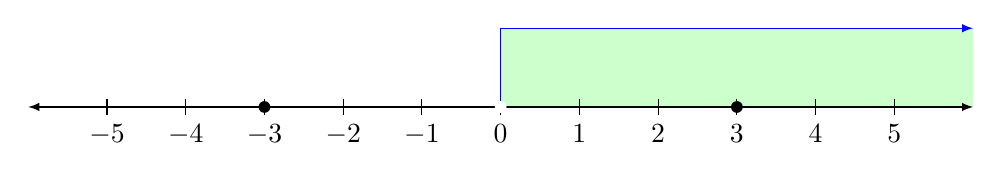
\begin{tikzpicture}
        \fill[green!20](6,0)rectangle(0,1);
        \draw[latex-latex] (-6,0) -- (6,0) ;
        \foreach \x in {-5,-4,-3,-2,-1,0,1,2,3,4,5} \draw[shift={(\x,0)},color=black] (0pt,3pt) -- (0pt,-3pt) node[below] {$\x$};
        \node[circle,fill=white,inner sep=1.5pt](a)at(0,0){};
        \node[circle,fill=black,inner sep=1.5pt](b)at(3,0){};
        \node[circle,fill=black,inner sep=1.5pt](c)at(-3,0){};
        \draw[-latex,blue](a)--++(0,1)--++(6,0);
    \end{tikzpicture}
    \caption{The domain is the green shaded area}
    \end{figure}
    Solve for $x$
    \begin{align*}
        2\log_4(x) &= \log_4(9)\\
        \log_4(x^2) &= \log_4(9))\\
        x^2&=9\\
        x&=\pm\sqrt{9}=\pm 3\\
    \end{align*}
    
    Ignore $x=-3$ since it's not in the domain of the problem. The only solution is $x=3$ and is verified graphically below.
    }
    \begin{figure}[htbp]
        \centering
        \includegraphics[width=0.6\textwidth]{log1_1}
        \caption{The solution to the problem is the intersection between $2\log_4(x) = \log_4(9)$}
        %\label{fig:myimage}
    \end{figure}


\begin{tcolorbox}[title=Solution, colback=blue!10!white, colframe=blue!75!black]
$x=3 $
\end{tcolorbox}

%     \begin{tcolorbox}[ams align*, colback=orange!60, colframe=blue]
% \text{The solution to the above equation is x=3 }
% \end{tcolorbox}

\newpage


    \item   $\log_2(x-1) - \log_2(x+1) = \log_2(3)$
    {\color{blue}
    \begin{align*}
       \log_2(x-1) - \log_2(x+1) &= \log_2(3) \\
       \log_2\left(\dfrac{x-1}{x+1}\right)&=\log_2(3)\\
       \dfrac{x-1}{x+1}&=3\\
       x-1&=3(x+1)\\
       x-1&=3x+3\\
       -4&=2x\\
       x&=-2
    \end{align*}
    }

    \begin{figure}[!h]
    \centering
    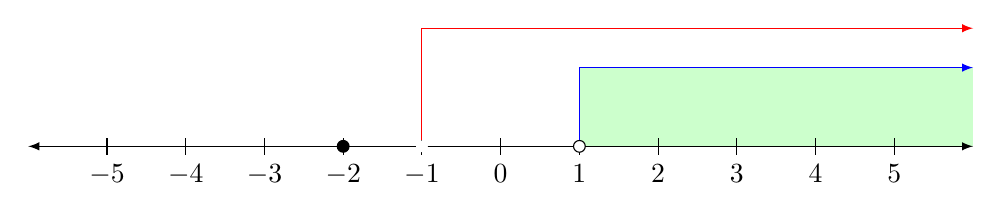
\begin{tikzpicture}
        \fill[green!20](6,0)rectangle(1,1);
        \draw[latex-latex] (-6,0) -- (6,0) ;
        \foreach \x in {-5,-4,-3,-2,-1,0,1,2,3,4,5} \draw[shift={(\x,0)},color=black] (0pt,3pt) -- (0pt,-3pt) node[below] {$\x$};
        \node[circle,fill=white,inner sep=1.5pt](a)at(-1,0){};
        \node[circle,draw,fill=white,inner sep=1.5pt](b)at(1,0){};
        \node[circle,draw,fill=black,inner sep=1.5pt](c)at(-2,0){};
        \draw[-latex,red](a)--++(0,1.5)--++(7,0);
        \draw[-latex,blue](b)--++(0,1)--++(5,0);
    \end{tikzpicture}
    \caption{The domain is the green shaded area}
    \end{figure}

    $x=-2$ is obviously not in the domain, so this problem does not any real solutions. 

\begin{tcolorbox}[title=Solution, colback=blue!10!white, colframe=blue!75!black]
No real solutions. 
\end{tcolorbox}


% \begin{tcolorbox}[ams align*, colback=orange!60, colframe=blue]
% \text{There are no real solutions to this problem.}
% \end{tcolorbox}

        
% \begin{tikzpicture}

% % Draw the number line with arrows
% \draw[<->, >=stealth] (-4,0) -- (4,0) node[below] {$x$};

% % Add tick marks and labels
% \foreach \x in {-3, -2, -1, 0, 1, 2, 3} {
%   \draw[shift={(\x,0)}, color=black] (0pt,3pt) -- (0pt,-3pt) node[below] {$\x$};
% }

% % Draw the domain for a specific example, e.g., [1, 3)
% % Replace with your specific domain and endpoints
% \draw[line width=2pt, blue] (1,0) node[circle, fill=blue, inner sep=1pt] {} -- (3,0) node[circle, fill=white, draw=blue, inner sep=1pt] {};

% \end{tikzpicture}

\newpage
    \item   $\log_3(x) + \log_3(x+2) = \log_3(15)$:\\
    {\color{blue}
    
    Let's look at the domain first: \\
    $\log_3(x): x > 0$\\
    $\log_3(x+2): x > -2$

    The overall domain is $x>0$ as shown in the figure below: 
    
    \begin{figure}[!h]
    \centering
    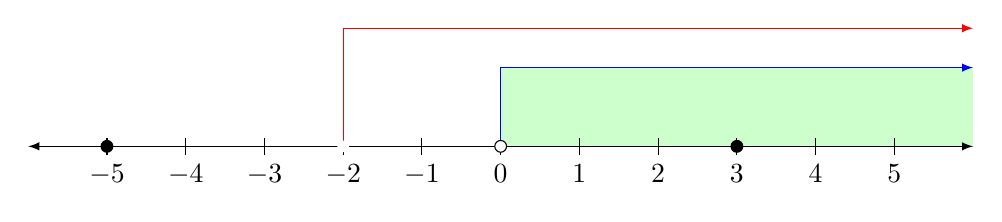
\begin{tikzpicture}
        \fill[green!20](6,0)rectangle(0,1);
        \draw[latex-latex] (-6,0) -- (6,0) ;
        \foreach \x in {-5,-4,-3,-2,-1,0,1,2,3,4,5} \draw[shift={(\x,0)},color=black] (0pt,3pt) -- (0pt,-3pt) node[below] {$\x$};
        \node[circle,fill=white,inner sep=1.5pt](a)at(-2,0){};
        \node[circle,draw,fill=white,inner sep=1.5pt](b)at(0,0){};
        \node[circle,draw,fill=black,inner sep=1.5pt](c)at(3,0){};
        \node[circle,draw,fill=black,inner sep=1.5pt](d)at(-5,0){};

        \draw[-latex,red](a)--++(0,1.5)--++(8,0);
        \draw[-latex,blue](b)--++(0,1)--++(6,0);
    \end{tikzpicture}
    \caption{The domain is the green shaded area}
    \end{figure}

    \begin{align*}
        \log_3(x) + \log_3(x+2) &= \log_3(15)\\
        \log_3(x(x+2))&=\log_3(15)\\
        x(x+2)&=15\\
        x^2+2x-15&=0\\
        (x+5)(x-3)&=0\\
        x&=-5;x=3
    \end{align*}
    
    Ignore $x=-5$ since it's not in the domain of the problem
    }
    \begin{figure}[htbp]
        \centering
        \includegraphics[width=0.6\textwidth]{log1_1}
        \caption{The solution to the problem is the intersection between $\log_3(x)+\log_3(x+2)$ and $\log_3(15)$}
        %\label{fig:myimage}
    \end{figure}

\begin{tcolorbox}[title=Solution, colback=blue!10!white, colframe=blue!75!black]
$x=3 $
\end{tcolorbox}

%     \begin{tcolorbox}[ams align*, colback=orange!60, colframe=blue]
% \text{The solution to the above equation is x=3 }
% \end{tcolorbox}

\newpage

    \item   $\log_5(x+3) + \log_5(x-3) = \log_5(16)$:
    {\color{blue}
  
    Let's look at the domain first: \\
    $\log_3(x+3): x > -3$\\
    $\log_3(x-3): x > 3$

    The overall domain is $x>3$ as shown in the figure below: 
    
    \begin{figure}[!h]
    \centering
    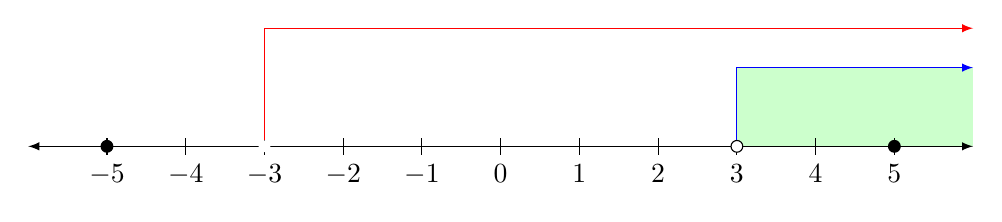
\begin{tikzpicture}
        \fill[green!20](6,0)rectangle(3,1);
        \draw[latex-latex] (-6,0) -- (6,0) ;
        \foreach \x in {-5,-4,-3,-2,-1,0,1,2,3,4,5} \draw[shift={(\x,0)},color=black] (0pt,3pt) -- (0pt,-3pt) node[below] {$\x$};
        \node[circle,fill=white,inner sep=1.5pt](a)at(-3,0){};
        \node[circle,draw,fill=white,inner sep=1.5pt](b)at(3,0){};
        \node[circle,draw,fill=black,inner sep=1.5pt](c)at(5,0){};
        \node[circle,draw,fill=black,inner sep=1.5pt](d)at(-5,0){};
        \draw[-latex,red](a)--++(0,1.5)--++(9,0);
        \draw[-latex,blue](b)--++(0,1)--++(3,0);
    \end{tikzpicture}
    \caption{The domain is the green shaded area}
    \end{figure}

    \begin{align*}
        \log_5(x) + \log_5(x+2) &= \log_5(16)\\
        \log_5((x+3)(x-3))&=\log_5(16)\\
        (x+3)(x-3)&=16\\
        x^2-9&=16\\
        x^2&=25\\
        x&=\pm\sqrt{25}=\pm 5
    \end{align*}
    
    Ignore $x=-5$ since it's not in the domain of the problem
    }
    \begin{figure}[htbp]
        \centering
        \includegraphics[width=0.6\textwidth]{log1_2}
        \caption{The solution to the problem is the intersection between $\log_5(x+3) + \log_5(x-3)$ and $\log_5(16)$}
        %\label{fig:myimage}
    \end{figure}


\begin{tcolorbox}[title=Solution, colback=blue!10!white, colframe=blue!75!black]
$x=5 $
\end{tcolorbox}

%     \begin{tcolorbox}[ams align*, colback=orange!60, colframe=blue]
% \text{The solution to the above equation is x=5 }
% \end{tcolorbox}

\newpage
    \item  $\log_{x-1}(x+1) + \log_{x+1}(x-1) = \frac{5}{2}$
    
    {\color{blue}
    Let's look at the domain first. The base of the log and the argument must both be positive: \\
    $x+1>0\Rightarrow   x > -1$\\
    $x-1>0\Rightarrow  x>-1$

    The overall domain is $x>1$ as shown in the figure below: 
    
    \begin{figure}[!h]
    \centering
    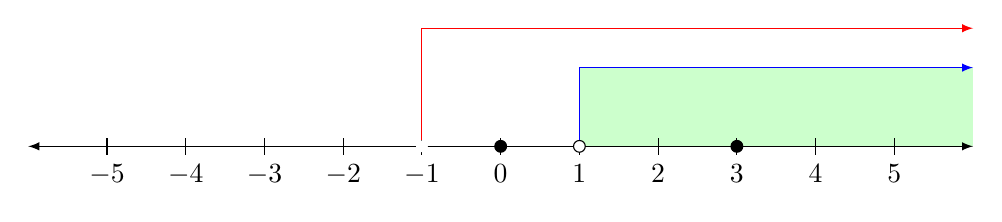
\begin{tikzpicture}
        \fill[green!20](6,0)rectangle(1,1);
        \draw[latex-latex] (-6,0) -- (6,0) ;
        \foreach \x in {-5,-4,-3,-2,-1,0,1,2,3,4,5} \draw[shift={(\x,0)},color=black] (0pt,3pt) -- (0pt,-3pt) node[below] {$\x$};
        \node[circle,fill=white,inner sep=1.5pt](a)at(-1,0){};
        \node[circle,draw,fill=white,inner sep=1.5pt](b)at(1,0){};
        \node[circle,draw,fill=black,inner sep=1.5pt](c)at(0,0){};
        \node[circle,draw,fill=black,inner sep=1.5pt](d)at(3,0){};
        \draw[-latex,red](a)--++(0,1.5)--++(7,0);
        \draw[-latex,blue](b)--++(0,1)--++(5,0);
    \end{tikzpicture}
    \caption{The domain is the green shaded area}
    \end{figure}

    Now let's solve the problem analytically and verify the solutions algebraically and graphically
    \begin{align*}
        \log_{x-1}(x+1) + \log_{x+1}(x-1) &= \frac{5}{2}\\
        \dfrac{\log_{x+1}(x+1)}{\log_{x+1}(x-1)}+\log_{x+1}(x-1)&=\frac{5}{2}\makebox[3cm]{\dotfill}\textit{Change of base}\\
        \dfrac{1}{\log_{x+1}(x-1)}+\log_{x+1}(x-1)&=\frac{5}{2}\makebox[3cm]{\dotfill}\textit{Identity Rule}\\
        1+\left(\log_{x+1}(x-1)\right)^2=\frac{5}{2}\log_{x+1}(x-1)\\
        \left(\log_{x+1}(x-1)\right)^2-\frac{5}{2}\log_{x+1}(x-1)+1=0\\
    \end{align*}
    We have a quadratic form. One way to solve it analytically is by doing a variable substitution. 
Let $u=\log_{x+1}(x-1)$
    \begin{align*}
        \left(\log_{x+1}(x-1)\right)^2-\frac{5}{2}\log_{x+1}(x-1)+1&=0\\
        u^2-\frac{5}{2}u+1&=0\\
        2u^2-5u+2&=0\\
        (2u-1)(u-2)&=0\\
        2u-1=0 ;&\quad u-2=0\\
        u=\frac{1}{2};&\quad u=2
    \end{align*}
We have two real solutions to the above quadratic formula:  $u=u_1=2$ or $u=u_2=\frac{1}{2}$. Now solve for $x$ for each value of $u$:
    \begin{align*}
        \log_{x+1}(x-1)&=u_1\\
        \log_{x+1}(x-1)&=2\\
        x-1&=(x+1)^2\\
        x-1&=x^2+2x+1\\
        x^2+x+2&=0
    \end{align*}

    The discriminant of the above quadratic equation is negative: 
    \[
        D=b^2-4ac=1^2-4(1)(1)=-3<0
    \]
    This means that $\log_{x+1}(x-1)=2$ has no real solutions. 
    
    Let's look at the other value of $u$:
    \begin{align*}
        \log_{x+1}(x-1)&=u_2\\
        \log_{x+1}(x-1)&=\frac{1}{2}\\
        x-1&=(x+1)^{1/2}\\
        x^2-2x+1&=x+1\\
        x^2-3x&=0\\
        x(x-3)&=0
    \end{align*}
We ignore $x=0$ since it's not in the domain. $x=3$ seems to be the only solution. Verify it algebraically:
    \begin{align*}
        \log_{x-1}(x+1) + \log_{x+1}(x-1) &= \frac{5}{2}\\
        \log_{3-1}(3+1) + \log_{3+1}(3-1)&\stackrel{?}{=}\frac{5}{2}\\
        \log_2(4)+\log_4(2)&\stackrel{?}{=}\frac{5}{2}\\
        \log_2(2^2)+\frac{1}{\log_2(4)}&\stackrel{?}{=}\frac{5}{2}\\
        \log_2(2^2)+\frac{1}{\log_2(2^2)}&\stackrel{?}{=}\frac{5}{2}\\
        2+\frac{1}{2} &\stackrel{?}{=}\frac{5}{2}\makebox[3cm]{\dotfill}\textit{TRUE}\\
    \end{align*}


        \begin{figure}[htbp]
        \centering
        \includegraphics[width=0.9\textwidth]{log1_3}
        \caption{Graphical solution to the equation $\log_{x-1}(x+1) + \log_{x+1}(x-1) = \frac{5}{2}$, which is the zero of the function.}
        %\label{fig:myimage}
    \end{figure}


\begin{tcolorbox}[title=Solution, colback=blue!10!white, colframe=blue!75!black]
$x=3 $
\end{tcolorbox}

%     \begin{tcolorbox}[ams align*, colback=orange!60, colframe=blue]
% \text{The solution to }\log_{x-1}(x+1) + \log_{x+1}(x-1) = \frac{5}{2} \text{ is } x=3 
% \end{tcolorbox}
}

\newpage
\item  $(\log_2(x))^2 - 5\log_2(x) + 6 = 0$:
      {\color{blue}
    
    Let's look at the domain first: \\
    $\log_2(x): x > 0$\\

    The domain is $x>0$ as shown in the figure below: 
    
    \begin{figure}[!h]
    \centering
    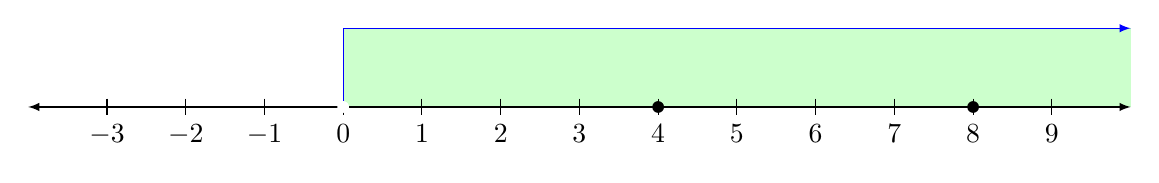
\begin{tikzpicture}
        \fill[green!20](10,0)rectangle(0,1);
        \draw[latex-latex] (-4,0) -- (10,0) ;
        \foreach \x in {-3,-2,-1,0,1,2,3,4,5,6,7,8,9} \draw[shift={(\x,0)},color=black] (0pt,3pt) -- (0pt,-3pt) node[below] {$\x$};
        \node[circle,fill=white,inner sep=1.5pt](a)at(0,0){};
        \node[circle,fill=black,inner sep=1.5pt](b)at(4,0){};
        \node[circle,fill=black,inner sep=1.5pt](c)at(8,0){};
        \draw[-latex,blue](a)--++(0,1)--++(10,0);
    \end{tikzpicture}
    \caption{The domain is the green shaded area}
    \end{figure}
 We have a quadratic form. One way to solve it analytically is by doing a variable substitution.     
 Let $u=\log_2(x)$
 \begin{align*}
        (\log_2(x))^2 - 5\log_2(x) + 6 &= 0
        u^2 - 5u + 6 = 0\\
        (u-3)(u-2)&=0\\
        u-3=0;&\quad u-2=0\\
        u=3&\quad u=32
    \end{align*}

   We have two real solutions to the above quadratic formula:  $u=u_1=3$ or $u=u_2=2$. Now solve for $x$ for each value of $u$:
    \begin{align*}
        \log_2(x)&=u_1\\
        \log_2(x)&=3\\
        x&=2^3\\
        x&=8
    \end{align*}
    \begin{align*}
        \log_2(x)&=u_2\\
        \log_2(x)&=4\\
        x&=2^2\\
        x&=4
    \end{align*}
    Both values of $x$ are acceptable since they are in the domain the function (they both lay in the gree region in the graph above).This is also verified graphically below:
    \newpage
    }
    \begin{figure}[htbp]
        \centering
        \includegraphics[width=0.8\textwidth]{log1_5}
        \caption{The solutions to the problem are the zeros of the function  $f(x)=(\log_2(x))^2 - 5\log_2(x) + 6 $}
        %\label{fig:myimage}
    \end{figure}

\begin{tcolorbox}[title=Solution, colback=blue!10!white, colframe=blue!75!black]
$x=4$ and $x=8$
\end{tcolorbox}

%     \begin{tcolorbox}[ams align*, colback=orange!60, colframe=blue]
% \text{The solutions to the above function are x=4 and x=8 }
% \end{tcolorbox}
    
\newpage
    \item  $\log_x(x+6) = \log_{x+6}(x) + \frac{1}{2}$
    {\color{blue}
    
    Let's look at the domain first: \\
    $ x > 0$\\
    $x+6>0\Rightarrow  x > -6$\\


    The domain is $x>0$ as shown in the figure below: 
    
    \begin{figure}[!h]
    \centering
    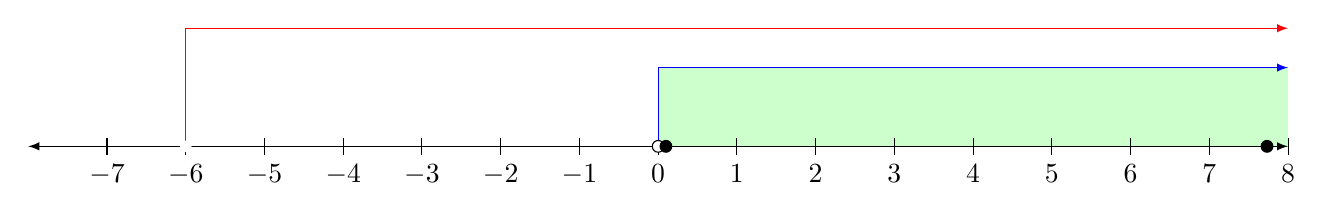
\begin{tikzpicture}
        \fill[green!20](8,0)rectangle(0,1);
        \draw[latex-latex] (-8,0) -- (8,0) ;
        \foreach \x in {-7,-6,-5,-4,-3,-2,-1,0,1,2,3,4,5,6,7,8} \draw[shift={(\x,0)},color=black] (0pt,3pt) -- (0pt,-3pt) node[below] {$\x$};
        \node[circle,fill=white,inner sep=1.5pt](a)at(-6,0){};
        \node[circle,draw,fill=white,inner sep=1.5pt](b)at(0,0){};
        \node[circle,draw,fill=black,inner sep=1.5pt](c)at(7.73276,0){};
        \node[circle,draw,fill=black,inner sep=1.5pt](d)at(0.09869,0){};

        \draw[-latex,red](a)--++(0,1.5)--++(14,0);
        \draw[-latex,blue](b)--++(0,1)--++(8,0);
    \end{tikzpicture}
    \caption{The domain is the green shaded area}
    \end{figure}
 We have a quadratic form. One way to solve it analytically is by doing a variable substitution.     
 Let $u=log_2(x)$
    \begin{align*}
        \log_x(x+6) &= \log_{x+6}(x) + \dfrac{1}{2}\\
        \log_x(x+6) &= \dfrac{\log_x(x)}{\log_x(x+6)}+\dfrac{1}{2}\\
        \log_x(x+6) &= \dfrac{1}{\log_x(x+6)}+\dfrac{1}{2}\\
        \left(\log_x(x+6)\right)^2 &= 1+\dfrac{1}{2}\log_x(x+6)\\
        \left(\log_x(x+6)\right)^2 &-\dfrac{1}{2}\log_x(x+6)-1=0\\
        2\left(\log_x(x+6)\right)^2 &-\log_x(x+6)-2=0\\
    \end{align*}
    We have a quadratic form. We can attempt to solve it analytically is by doing a variable substitution.     
 Let $u=\log_x(x+6)$
    \begin{align*}
        2\left(\log_x(x+6)\right)^2 &-\log_x(x+6)-2=0\\
        2u^2-u-2&=0\\
    \end{align*}
    Use the quadratic formula to solve for $u$:
    \begin{align*}
        u&=\dfrac{-b\pm\sqrt{b^2-4ac}}{2a}\\
        &=\dfrac{-(-1)\pm\sqrt{(-1)^2-4(2)(-2)}}{2(2)}\\
        &=\dfrac{1\pm\sqrt{17}}{4}\\
    \end{align*}
    We have two real values for $u: u_1 = (1-\sqrt{17})/4, \text{ and } u_2=(1+\sqrt{17})/4$.
    
    Since $u=\log_x(x+6)$, solving for $x$ 

    When we attempt to use these values of $u$to solve for $x$, we find that we have transcendental equations either in the form of logarithms or exponential:
    \[
    \log_x(x+6) = \dfrac{1\pm\sqrt{17}}{4}\Rightarrow x^{\frac{1\pm\sqrt{17}}{4}}=x+6
    \]
    
    These equations cannot be easily solved analytically. However, they can be solved graphically as shown in the figure below: Look for the intersection points between $log_x(x+6)$ and $\dfrac{1\pm\sqrt{17}}{4}$. 

    \begin{figure}[htbp]
        \centering
        \includegraphics[width=0.8\textwidth]{log1_7}
        \caption{Solutions to $\log_x(x+6)=u$ where $u=(1\pm\sqrt{17})/{4}$}
    \end{figure}

Another way to solve this problem is to graphically find the solutions by plotting both sides of the original equation and finding the intersection points. This is done in the figure below. The intersection points are are the same as the one in the above plot. 

    \begin{figure}[htbp]
        \centering
        \includegraphics[width=0.8\textwidth]{log1_6}
        \caption{The solutions to the problem are the zeros of the function  $f(x)=(\log_2(x))^2 - 5\log_2(x) + 6 $}
        %\label{fig:myimage}
    \end{figure}
}

\begin{tcolorbox}[title=Solution, colback=blue!10!white, colframe=blue!75!black]
$x=7.73276$
\end{tcolorbox}


\newpage
\item $\ln{t}+3\sqrt{\ln{t}}-10=0$

{\color{blue}
The domain of $\ln{t}$ is $t>0$\\
Let $u=\sqrt{\ln{t}}$, then $u^2=\ln{t}$. Substitute in the equation above
\[
u^2+3u-10=0
\]
Solve by factoring
\begin{align*}
    u^2+3u-10&=0\\
    (u+5)(u-2)&=0\\
    u=-5;&u=2
\end{align*}
But $u$ cannot be negative since it's a principal square root. So we reject $u=-5$. For $u=2$, we have
\begin{align*}
    u=2&=\sqrt{\ln{t}}\\
    4&=\ln{t}\\
    t&=e^{4}
\end{align*}

Check:\\
\begin{align*}
    \ln{t}+3\sqrt{\ln{t}}-10&\stackrel{?}{=}0\\
    \ln{e^4}+3\sqrt{\ln{e^4}}-10&\stackrel{?}{=}0\\
    4+3\sqrt{4}-10&\stackrel{?}{=}0\\
    4+3\cdot 2-10&\stackrel{?}{=}0\checkmark
\end{align*}

\fbox{The solution to this equation is $t=e^4$}
}
\newpage
\item $\left(\ln{w}\right)^2-\ln{w^5}=-6$

{\color{blue}
Simplify the equation by applying the power rule to the second term on the left and gathering all the terms on the left side of the equal sign.
\[
\left(\ln{w}\right)^2-5\ln{w}+6=0
\]
Let $u=\ln{w}$. The equation becomes 
\[
u^2-5u+6=0
\]
Factor the quadratic formula in $u$:
\begin{align*}
    u^2-5u+6&=0\\
    (u-3)(u-2)&=0\\
    u=3,&u=2
\end{align*}
Now obtain the values of $w$ for each of the $u$ values.\\
For $u=2$:
\begin{align*}
    u=2&=\ln{w}\\
    w&=e^2\\
\end{align*}
For $u=3$:
\begin{align*}
    u=3&=\ln{w}\\
    w&=e^3\\
\end{align*}

Both values of $w$ are acceptable, but we still have to check those values to ensure that they satisfy the given equation.\\
Check $w=e^2$:\\
\begin{align*}
    \left(\ln{w}\right)^2-\ln{w^5}&=-6\\
    \left(\ln{e^2}\right)^2-\ln\left(\left(e^2\right)^5\right)&\stackrel{?}{=}-6\\
    (2)^2-\ln{e^{10}}\stackrel{?}{=}-6\\
    4-10\stackrel{?}{=}-6\checkmark
\end{align*}
Check $w=e^3$:\\
\begin{align*}
    \left(\ln{w}\right)^2-\ln{w^5}&=-6\\
    \left(\ln{e^3}\right)^2-\ln\left(\left(e^3\right)^5\right)&\stackrel{?}{=}-6\\
    (3)^2-\ln{e^{15}}\stackrel{?}{=}-6\\
    9-15\stackrel{?}{=}-6\checkmark
\end{align*}

}

%     \begin{tcolorbox}[ams align*, colback=orange!60, colframe=blue]
% \text{The solutions to the above function are x=0.09869 and x=7.73276 }
% \end{tcolorbox}
    
   \end{enumerate} 
% \chead{Expand Completely}

\newpage
%%%%%%%%%%%%%%%%%%%%%%%%%%%%%%%%%%%%%%%%%%%%%%%%%%%%%%%%%%%%%%%%%%%%%%%%%%%%%%%
%%%
%%%                     EXPAND COMPLETELY
%%%
%%%%%%%%%%%%%%%%%%%%%%%%%%%%%%%%%%%%%%%%%%%%%%%%%%%%%%%%%%%%%%%%%%%%%%%%%%%%%%%
\noindent\subsection*{Solve Exponential Problems}
\begin{tcolorbox}[title=Note, colback=blue!10!white, colframe=blue!75!black]
Use the properties to write in simplest form. In particular, use the power, product and quotient rules. 
\end{tcolorbox}
\vspace{3.6cm}
\begin{enumerate}[resume]
    \item  $2^{x+1}=6^x$:
    {\color{blue}
    \begin{align*}
        2^{x+1}&=6^x\\
        \ln{2^{x+1}}&=\ln{6^x}\makebox[5cm]{\dotfill}\textit{Equality of Base}\\
        (x+1)\ln{2}&=x\ln{6}\makebox[5cm]{\dotfill}\textit{Power Rule}\\
        x\ln{2}+\ln{2}&=x\ln{6}\\
        x(\ln{2}-\ln{6})&=-\ln{2}\\
        x&=\dfrac{-\ln{2}}{\ln{2}-\ln{6}}\\
        \Aboxed{x&=\dfrac{\ln{2}}{\ln{6}-\ln{2}}}
    \end{align*}
    }


    
    \item  $5\cdot 2^{2x-1}=7^{x+1}$:
    {\color{blue}
        \begin{align*}
        5\cdot 2^{2x-1}&=7^{x+1}\\
        \ln{5\cdot 2^{2x-1}}&=\ln{7^{x+1}}\makebox[5cm]{\dotfill}\textit{Equality of Base}\\
        \ln{5}+\ln{2^{2x-1}}&=\ln{7^{x+1}}\makebox[5cm]{\dotfill}\textit{Power Rule}\\
        \ln{5}+(2x1)\ln{2}&=(x+1)\ln{7}\makebox[5cm]{\dotfill}\textit{Power Rule}\\
        \ln{5}+2x\ln{2}+\ln{2}&=x\ln{7}=\ln{7}\\
        2x\ln{2}-x\ln{7}&=\ln{7}-\ln{5}-\ln{2}\\
        x(2\ln{2}-\ln{7})&=\ln7-\ln{5}-\ln{2}\\
        \Aboxed{x&=\dfrac{\ln{7}-\ln{5}-\ln{2}}{2\ln{2}-\ln{7}}}        
    \end{align*}
    }



    \item  $3\cdot 5^{3x-1}=9^{x+2}$:
    
        {\color{blue}
        \begin{align*}
        3\cdot 5^{3x-1}&=9^{x+2}\\
        \ln{\left(3\cdot 5^{3x-1}\right)}&=\ln{\left(9^{x+2}\right)}\makebox[5cm]{\dotfill}\textit{Equality of Base}\\ 
        \ln{3}+\ln{5^{3x-1}}&=\ln{9^{x+2}}\makebox[5cm]{\dotfill}\textit{Product Rule}\\ 
        \ln{3}+(3x-1)\ln{5}&=(x+2)\ln{9}\makebox[5cm]{\dotfill}\textit{Power Rule}\\ 
        \ln{3}+3x\ln{5}-\ln{5}&=x\ln{9}+2\ln{9}\\
        3x\ln{5}-x\ln{3^2}&=\ln{5}-\ln{3}+2\ln{3^2}\\
        x(3\ln{5}-2\ln{3})&=\ln{5}-\ln{3}+4\ln{3}\makebox[5cm]{\dotfill}\textit{Power Rule}\\ 
        x(3\ln{5}-2\ln{3})&=\ln{5}+3\ln{3}\\
        \Aboxed{x&=\dfrac{\ln{5}+3\ln{3}}{{3\ln{5}-2\ln{3}}}}
    \end{align*}
    }
    
    
    OR
    {\color{teal}
    
        \begin{align*}
        3\cdot 5^{3x-1}&=9^{x+2}\\
        5^{3x-1}&=\dfrac{9^{x+2}}{3}\\
        \ln{5^{3x-1}}&=\ln{\dfrac{9^{(x+2)}}{3}}\makebox[5cm]{\dotfill}\textit{Equality of Base}\\
        \ln{5^{3x-1}}&=\ln{9^{x+2}}-\ln{3}\makebox[5cm]{\dotfill}\textit{Quotient Rule}\\ 
         (3x-1)\ln{5}&=(x+2)\ln{9}-\ln{3}\makebox[5cm]{\dotfill}\textit{Power Rule}\\ 
         3x\ln{5}-\ln{5}&=x\ln{9}+2\ln{9}-\ln{3}\\
         3x\ln{5}-\ln{5}&=x\ln{3^2}+2\ln{3^2}-\ln{3}\\
         3x\ln{5}-\ln{5}&=2x\ln{3}+4\ln{3}-\ln{3}\makebox[5cm]{\dotfill}\textit{Power Rule}\\
         3x\ln{5}-2x\ln{3}&=\ln{5}+3\ln{3}\\
         x(3\ln{5}-2\ln{3})&=\ln{5}+3\ln{3}\\
         \Aboxed{x&=\dfrac{\ln{5}+3\ln{3}}{3\ln{5}-2\ln{3}}}
    \end{align*}
    }
OR\\

    {\color{orange}
    
        \begin{align*}
        3\cdot 5^{3x-1}&=9^{x+2}\\
        5^{3x-1}&=\dfrac{\left(3^2\right)^{(x+2)}}{3}\\
        5^{3x-1}&=\dfrac{3^{2(x+2)}}{3}\makebox[5cm]{\dotfill}\textit{Power Rule}\\ 
        5^{3x-1}&=\dfrac{3^{2x+4}}{3}\\
        5^{3x-1}&=3^{2x+4-1}\\
        5^{3x-1}&=3^{2x+3}\\
        \ln 5^{3x-1}&=\ln 3^{2x+3}\makebox[5cm]{\dotfill}\textit{Equality of Base}\\
        (3x-1)\ln{5}&=(2x+3)\ln{3}\\
        3x\ln{5}-\ln{5}&=2x\ln{3}+3\ln{3}\\
        3x\ln{5}-2x\ln{3}=&\ln{5}+3\ln{3}\\
        x(3\ln{5}-2\ln{3})&=\ln{5}+3\ln{3}\\
        \Aboxed{x&=\dfrac{\ln{5}+3\ln{3}}{3\ln{5}-2\ln{3}}}
    \end{align*}
    }



    \item  $5\cdot 2^{2x-1}=7^{x+1}$:
    {\color{blue}
        \begin{align*}
        5\cdot 2^{2x-1}&=7^{x+1}\\
        \ln{5\cdot 2^{2x-1}}&=\ln{7^{x+1}}\makebox[5cm]{\dotfill}\textit{Equality of Base}\\
        \ln{5}+\ln{2^{2x-1}}&=\ln{7^{x+1}}\makebox[5cm]{\dotfill}\textit{Power Rule}\\
        \ln{5}+(2x1)\ln{2}&=(x+1)\ln{7}\makebox[5cm]{\dotfill}\textit{Power Rule}\\
        \ln{5}+2x\ln{2}+\ln{2}&=x\ln{7}=\ln{7}\\
        2x\ln{2}-x\ln{7}&=\ln{7}-\ln{5}-\ln{2}\\
        x(2\ln{2}-\ln{7})&=\ln7-\ln{5}-\ln{2}\\
        \Aboxed{x&=\dfrac{\ln{7}-\ln{5}-\ln{2}}{2\ln{2}-\ln{7}}}        
    \end{align*}
    }








    
    \item  $e^{2x}+4e^x=12$:
    {\color{blue}
        \begin{align*}
        e^{2x}+4e^x&=12\\
        \left(e^x\right)^2+4e^x7-12&=0\makebox[5cm]{\dotfill}\textit{Power Rule}\\
        u^2+4u-12&=0\makebox[5cm]{\dotfill}\text{let }u = e^x>0\\
        (u+6)(u-2)&=0\\
        u=-6&;u=2
    \end{align*}
Since $u=e^x$, which is always positive, we reject $u=-6$ as a solution and keep $u=2$ to solve for $x$. 

\begin{align*}
    u=e^x&=2\\
    \ln{e^x}&=\ln{2}\makebox[5cm]{\dotfill}\textit{Equality of Base}\\
    \Aboxed{x&=\ln{2}\makebox[5cm]{\dotfill}\textit{Power Rule}}
\end{align*}

Check:

\begin{align*}
    e^{2x}+4e^x&=12\\
    e^{2\ln{2}}+4e^{\ln{2}}&\stackrel{?}{=}12\\
    e^{\ln{2^2}}+4e^{\ln{2}}&\stackrel{?}{=}12\\
    2^2+4(2)&\stackrel{?}{=}12\\
    4+8&\stackrel{?}{=}12\checkmark
\end{align*}


    }

    
    \item  $\dfrac{e^x+e^{-x}}{2}=3$:
    {\color{blue}
        \begin{align*}
        \dfrac{e^x+e^{-x}}{2}&=3\\
        e^x+e^{-x}&=6\\
        e^x+\dfrac{1}{e^x}&=6\\
        \dfrac{e^{2x}+1}{e^x}&=6\\
        e^{2x}+1&=6e^x\\
        \left(e^{x}\right)^2-&6e^x+1=0\makebox[5cm]{\dotfill}\textit{Power Rule}
    \end{align*}

    
    Let $u=e^x$, then the equation becomes
    \[
        u^2-6x+1=0
    \]
Use the quadratic formula
\begin{align*}
    u&=\dfrac{-b\pm\sqrt{b^2-4ac}}{2a}\\
    &=\dfrac{-(-6)\pm\sqrt{(-6)^2-4(1)(1)}}{2(1)}\\
    &=\dfrac{6\pm\sqrt{36-4}}{2}\\
    &=\dfrac{6\pm\sqrt{32}}{2}\\
    &=\dfrac{6\pm 4\sqrt{2}}{2}\\
    &=3\pm 2\sqrt{2}
\end{align*}
Back to $x$: $u=e^x=3\pm2\sqrt{2}$. Both vales $3+2\sqrt{2}$ and $3-2\sqrt{2}$ are positive, so they are both solutions to the problem. 

\begin{align*}
    e^x&=3\pm 2\sqrt{2}\\
    \ln{e^x}&=\ln{3\pm 2\sqrt{2}}\makebox[5cm]{\dotfill}\textit{Equality of Base}\\
    \Aboxed{x&=\ln{3\pm 2\sqrt{2}}\makebox[5cm]{\dotfill}\textit{Inverse Rule}}
\end{align*}

}
    


\end{enumerate}
% \subsubsection*{Word Problems}
\chead{Word Problems}

\begin{enumerate}[resume]

\item \textbf{Sound Intensity:} The decibel level of a sound is given by $L = 10\log\left(\frac{I}{I_0}\right)$, in dB,  where $I$ is the intensity of the sound, in W/m$^2$,  and $I_0 = 10^{-12}$ W/m$^2$ is the threshold of hearing. If a rock concert measures 115 dB, what is the intensity of the sound?

{\color{blue}

Plug $L=115 $dB and  $I_0 = 10^{-12}$ W/m$^2$ into the equation and solve for $I$. There is no need to carry the  units around. All the terms in the proper units so the result will be in its proper units.

\begin{align*}
    115 &= 10\log\left(\frac{I}{10^{-12}}\right) \\
    11.5 &= \log\left(\frac{I}{10^{-12}}\right) \\
    10^{11.5} &= \frac{I}{10^{-12}} \\
    I &= 10^{11.5} \times 10^{-12} = 10^{-0.5} \\
    I &\approx 0.316 \text{ W/m}^2
\end{align*}

\fbox{$I=0.32 $W/m$^2$}}

% \begin{tcolorbox}[title=Solution, colback=blue!10!white, colframe=blue!75!black]
% $I=0.32 $W/m$^2$
% \end{tcolorbox}

% -------------------------------------------------------------------------------

\newpage
\item \textbf{Radioactive Decay:} Carbon-14 has a half-life of 5,730 years. If a fossil contains 30\% of its original Carbon-14, how old is the fossil? Use the formula $N(t) = N_0 e^{-kt}$ where $N_0$ is the amount of original sample, $k$ is the radio active decay constant, and $t$ is time in years. 

{\color{blue}

Use the half-life to compute $k$: 50\% of the sample is gone, and thus 50\% is left, after 5,730 years.
    \begin{align*}
        0.5 N_0 &= N_0 e^{-k(5730)} \\
        0.50 &= e^{-5730k} \\
        \ln(0.5)&=-5730k\\
        k&=\dfrac{\ln(0.5)}{-5730}\approx 0.00012097
    \end{align*}

Now use this value of $k$ throughout the problem to find $t$ when $N_0=0.3N$. 
    \begin{align*}
        0.30 N_0 &= N_0 e^{-kt} \\
        0.30 &= e^{-0.00012097t} \\
        \ln(0.30) &= -0.00012097t \\
        t &= \frac{\ln(0.30)}{-0.00012097} \\
        t &\approx 9,953 \text{ years}
    \end{align*}

\fbox{$t=9,953$ years.}}
% \begin{tcolorbox}[title=Solution, colback=blue!10!white, colframe=blue!75!black]
% $t=9,953$ years.
% \end{tcolorbox}

% -------------------------------------------------------------------------------

\newpage
\item \textbf{Population Growth:} A city's population grows according to $P(t) = P_0 e^{0.025t}$, where $t$ is in years, and $P_0$ is the initial population. How long will it take for the population to triple?

{\color{blue}
Find $t$ when $P=3P_0$
    \begin{align*}
        3P_0 &= P_0 e^{0.025t} \\
        3 &= e^{0.025t} \\
        \ln(3) &= 0.025t \\
        t &= \frac{\ln(3)}{0.025} \\
        t &\approx 43.94 \text{ years}
        \end{align*}


\fbox{$t=43.94$ years.}}
% \begin{tcolorbox}[title=Solution, colback=blue!10!white, colframe=blue!75!black]
% $t=43.94$ years.
% \end{tcolorbox}
% -------------------------------------------------------------------------------

\newpage
\item \textbf{Compound Interest:} An investment of \$5,000 earns 6\% annual interest compounded monthly. How long will it take for the investment to grow to \$8,000? Use $A = P\left(1 + \frac{r}{n}\right)^{nt}$.

{\color{blue}
Find $t$ when $P=\$5,000$, $r=0.06$, $n=12$ (compounded monthly), and $A=\$8,000 $

\begin{align*}
8000 &= 5000\left(1 + \frac{0.06}{12}\right)^{12t} \\
1.6 &= (1.005)^{12t} \\
\ln(1.6) &= \ln\left(1.005)^{12t}\right) \\
\ln(1.6) &= 12t \ln(1.005) \\
t &= \frac{\ln(1.6)}{12\ln(1.005)} \\
t &\approx 7.85 \text{ years}
\end{align*}

\fbox{$t=7.85$ years.}}
% \begin{tcolorbox}[title=Solution, colback=blue!10!white, colframe=blue!75!black]
% $t=7.85$ years.
% \end{tcolorbox}


% -------------------------------------------------------------------------------

\newpage
\item \textbf{Sound Intensity:} A library has a noise level of 40 dB and a busy street has a noise level of 70 dB. How many times more intense is the sound on the busy street compared to the library?


{\color{blue}

    Let $L_1=40$ dB be the noise level in the library and $L_2=70$ dB be the noise level on a busy street. 
    
    Let $L_1=40$ dB be the noise level in the library
    \begin{align*}
        L_1 &= 10\log\left(\frac{I_1}{I_0}\right) = 40 \\
        &\log\left(\frac{I_1}{I_0}\right) = 4
    \end{align*}

    $L_2=70$ dB be the noise level on a busy street. 
    \begin{align*}
        L_2 &= 10\log\left(\frac{I_2}{I_0}\right) = 70 \\
        &\log\left(\frac{I_2}{I_0}\right) = 7 \\
    \end{align*}
    
    Subtract the two equations
    \begin{align*}
       \log\left(\frac{I_2}{I_0}\right)- \log\left(\frac{I_1}{I_0}\right)&= 7-4 \\
       \log\left(\dfrac{\frac{I_2}{I_0}}{\frac{I_1}{I_0}}\right)&=3\\
       \log\left(\dfrac{\frac{I_2}{\cancel{I_0}}}{\frac{I_1}{\cancel{I_0}}}\right)&=3\\
       \log\left(\dfrac{I_2}{I_1}\right)&=3\\
       \dfrac{I_2}{I_1}&=10^3=1,000\\
    \end{align*}

\fbox{1,000 times more intense}}
% \begin{tcolorbox}[title=Solution, colback=blue!10!white, colframe=blue!75!black]
% 1,000 times more intense
% \end{tcolorbox}
% -------------------------------------------------------------------------------

\newpage
\item \textbf{Radioactive Decay:} Plutonium-239 has a half-life of 24,100 years. How long will it take for a sample to decay to 10\% of its original amount?

{\color{blue}
\begin{align*}
k &= \frac{\ln(2)}{24100} \\
0.10 &= e^{-kt} \\
\ln(0.10) &= -\frac{\ln(2)}{24100}t \\
t &= \frac{24100 \ln(0.10)}{-\ln(2)} \\
t &\approx 80,061 \text{ years}
\end{align*}


\fbox{$t=80,061$ years.}}
% \begin{tcolorbox}[title=Solution, colback=blue!10!white, colframe=blue!75!black]
% $t=80,061$ years. 
% \end{tcolorbox}

% -------------------------------------------------------------------------------

\newpage
\item \textbf{Logistic Growth:} A population of bacteria grows according to $P(t) = \frac{5000}{1 + 49e^{-0.8t}}$, where $t$ is in hours. How long will it take for the population to reach 4,000?

{\color{blue}
    
    \begin{align*}
        4000 &= \frac{5000}{1 + 49e^{-0.8t}} \\
        1 + 49e^{-0.8t} &= \dfrac{5000}{4000} \\
        1 + 49e^{-0.8t} &= 1.25 \\
        49e^{-0.8t} &= 0.25 \\
        e^{-0.8t} &= \dfrac{0.25}{49} \\
        -0.8t &= \ln\left(\frac{0.25}{49}\right) \\
        t &= \frac{\ln(0.25/49)}{-0.8} \\
        t &\approx 6.61 \text{ hours}
    \end{align*}


\fbox{The population will reach 4,000 in $t=6.61$ hours}}

% \begin{tcolorbox}[title=Solution, colback=blue!10!white, colframe=blue!75!black]
% The population will reach 4,000 in $t=6.61$ hours
% \end{tcolorbox}
% -------------------------------------------------------------------------------

\newpage
\item \textbf{Compound Interest:} You invest \$10,000 at 4.5\% annual interest. Compare the time it takes to double your money when compounded (a) annually, (b) quarterly, and (c) continuously (use $A = Pe^{rt}$ for continuous compounding and $A=P\left(1+\dfrac{r}{n}\right)^{rt}$).

{\color{blue}
Obtain a general equation for $t$ for both situation then plug in the specific values for each situation.

For the compound interest
\begin{align*}
    A &= P\left(1+\dfrac{r}{n}\right)^{nt}\\
    \dfrac{A}{P}&=\left(1+\dfrac{r}{n}\right)^{nt}\\
    \ln\left(\dfrac{A}{P}\right)&=\ln\left(1+\dfrac{r}{n}\right)^{nt}\\
    \ln\left(\dfrac{A}{P}\right)&=(n\,t)\ln\left(1+\dfrac{r}{n}\right)\\
    t&=\dfrac{\ln\left(\dfrac{A}{P}\right)}{n\cdot \ln\left(1+\dfrac{r}{n}\right)}\\
\end{align*}
For continuous compounding:
\begin{align*}
    A &= Pe^{rt}\\
    \dfrac{A}{P}&=e^{rt}\\
    \ln\left(\dfrac{A}{P}\right)&=rt\\
    t&=\dfrac{1}{r}\ln\left(\dfrac{A}{P}\right)\\
\end{align*}

\begin{align*}
\text{(a) Annually: $n=1$;}&\quad  t=\dfrac{\ln\left(\dfrac{2000}{10000}\right)}{1\cdot \ln\left(1+\dfrac{0.045}{1}\right)}\approx 15.75 \text{ years}\\
\text{(b) Quarterly: $n=4$;}&\quad t=\dfrac{\ln\left(\dfrac{2000}{10000}\right)}{4\cdot \ln\left(1+\dfrac{0.045}{4}\right)}\approx 15.52 \text{ years}\\
\text{(c) Continuously: }&\quad t=\dfrac{1}{0.045}\ln\left(\dfrac{2000}{10000}\right) \approx 15.40 \text{ years}
\end{align*}

\fbox{(a) 15.75 years, (b) 15.52 years, (c) 15.40 years}}
% \begin{tcolorbox}[title=Solution, colback=blue!10!white, colframe=blue!75!black]
% \textbf{Answer:} (a) 15.75 years, (b) 15.52 years, (c) 15.40 years
% \end{tcolorbox}
% -------------------------------------------------------------------------------

\newpage
\item \textbf{Population Growth:} The population of a town was 25,000 in 2010 and 32,000 in 2020. Assuming exponential growth $P(t) = P_0 e^{kt}$, what will the population be in 2030?

{\color{blue}
Use the given information to compute $k$ the use it to compute the answer.\\
The initial population is $P_0=25,000$. 10 years later, the population $P(10)=32,000$. Plug the numbers in and get $k$:

\begin{align*}
32000 &= 25000e^{10k} \\
1.28 &= e^{10k} \\
10k &= \ln(1.28)\\
k&=\dfrac{\ln(1.28)}{10} \approx 0.02469
\end{align*}

Now get the population after 30 years

\begin{align*}
P(30) &= 25000e^{0.02469(30)} \\
P(30) &\approx 51,968
\end{align*}


\fbox{The population in 20230 would be 51,968 people.}}

% \begin{tcolorbox}[title=Solution, colback=blue!10!white, colframe=blue!75!black]
% The population in 20230 would be 51,968 people.
% \end{tcolorbox}
% -------------------------------------------------------------------------------

\newpage
\item \textbf{Sound Intensity:} The sound intensity level increases by 3 dB. By what factor does the actual intensity increase?

{\color{blue}
Let $L_1$ be the original sound level with intensity $I_1$ and $L_2$ the new sound level with intensity $I_2$, which is 3 dB higher.  
\[
L_1=10\log\left(\dfrac{I_1}{I_0}\right)
\]
\[
L_2=10\log\left(\dfrac{I_2}{I_0}\right)
\]
Given $L_2-L_1=3$ dB

    \begin{align*}
       3&=10\log\left(\frac{I_2}{I_0}\right)- 10\log\left(\frac{I_1}{I_0}\right)\\
       3&=10\log\left(\dfrac{\frac{I_2}{I_0}}{\frac{I_1}{I_0}}\right)\\
       \dfrac{3}{10}&=\log\left(\dfrac{\frac{I_2}{\cancel{I_0}}}{\frac{I_1}{\cancel{I_0}}}\right)\\
       0.3&=\log\left(\dfrac{I_2}{I_1}\right)\\
       10^{0.3}&=\dfrac{I_2}{I_1}\\
       \dfrac{I_2}{I_1}&\approx 2.00
    \end{align*}


\fbox{The intensity increases by a factor of 2}}
% \begin{tcolorbox}[title=Solution, colback=blue!10!white, colframe=blue!75!black]
% The intensity increases by a factor of 2
% \end{tcolorbox}
% -------------------------------------------------------------------------------

\newpage
\item \textbf{Radioactive Decay:} Iodine-131 is used in medical treatments and has a half-life of 8 days. A patient receives a 50 mCi dose. How long will it take for the radioactivity to decrease to a safe level of 2 mCi?


{\color{blue}
Use $N(t)=N_0\,2^{-t/t_0}$, where $N_0$ is the initial amount and $t_0$ is the half-life of the substance. 
\begin{align*}
2 &= 50 \cdot 2^{-t/8} \\
\dfrac{2}{50} &= 2^{t/8} \\
0.04&= 2^{t/8} \\
\log(0.04) &= -\frac{t}{8}\log(2) \\
t &= -\frac{8\log(0.04)}{\log(2)} \\
t &\approx 37.29 \text{ days}
\end{align*}


\fbox{It will take 37.29 days for the radioactivity to decrease to safe levels.} }

% \begin{tcolorbox}[title=Solution, colback=blue!10!white, colframe=blue!75!black]
% It will take 37.29 days for the radioactivity to decrease to safe levels. 
% \end{tcolorbox}

% -------------------------------------------------------------------------------

\newpage
\item \textbf{Compound Interest:} Which investment will grow faster: \$5,000 at 7\% compounded quarterly or \$5,000 at 6.9\% compounded continuously? Calculate the value of each after 10 years.

{\color{blue}
The present value $P$ for both cases is \$5,000. The interest rate is $r_1=0.07$ for quarterly ($n=4$) compounding, while it's $r_2=0.069$ for continuous compounding. $t=10$ years for both. 

\begin{align*}
\text{Quarterly: } A_1 &=P\left(1+\dfrac{r_1}{n}\right)^{nt}\\
&= 5000\left(1 + \frac{0.07}{4}\right)^{4\times 10} \\
&\approx \$10,048.27 \\
\text{Continuously: } A_2&=Pe^{r_2t}\\
                 &= 5000e^{0.069(10)} \\
                 &\approx \$9,922.75
\end{align*}


\fbox{7\% compounded quarterly grows faster; \$10,048.27 vs \$9,922.75}}
% \begin{tcolorbox}[title=Solution, colback=blue!10!white, colframe=blue!75!black]
% 7\% compounded quarterly grows faster; \$10,048.27 vs \$9,922.75
% \end{tcolorbox}
% -------------------------------------------------------------------------------

\newpage
\item \textbf{Logistic Growth:} A fish population in a lake follows the logistic model $P(t) = \frac{8000}{1 + 15e^{-0.5t}}$, where $t$ is in years. When will the population reach 6,000 fish?

{\color{blue}

\begin{align*}
    6000 &= \frac{8000}{1 + 15e^{-0.5t}} \\
    1 + 15e^{-0.5t} &= \dfrac{8000}{6000} \\
    1 + 15e^{-0.5t} &= \frac{4}{3}-1 \\
    15e^{-0.5t} &= \frac{1}{3}\\
    e^{-0.5t} &= \frac{1}{15\times 3} \\
    e^{-0.5t} &= \frac{1}{45} \\
    -0.5t&=-\ln{(45)}\makebox[3cm]{\dotfill}\textit{$\ln(1/x)=-\ln(x)$}\\
    t &= \frac{\ln(45)}{0.5} \\
    t &\approx 7.62 \text{ years}
\end{align*}

\fbox{The population will reach 6,000 fish in 7.62 years}}

% \begin{tcolorbox}[title=Solution, colback=blue!10!white, colframe=blue!75!black]
% The population will reach 6,000 fish in 7.62 years
% \end{tcolorbox}
% -------------------------------------------------------------------------------

\newpage
\item \textbf{pH Levels:} The pH of a solution is given by $\text{pH} = -\log[H^+]$, where $[H^+]$ is the hydrogen ion concentration in moles per liter. If a solution has a pH of 3.5, what is the hydrogen ion concentration?

{\color{blue}
\begin{align*}
3.5 &= -\log[H^+] \\
-3.5 &= \log[H^+] \\
[H^+] &= 10^{-3.5} \\
[H^+] &\approx 3.16 \times 10^{-4} \text{ mol/L}
\end{align*}



\fbox{$3.16 \times 10^{-4}$ mol/L}}
% \begin{tcolorbox}[title=Solution, colback=blue!10!white, colframe=blue!75!black]
% $3.16 \times 10^{-4}$ mol/L\end{tcolorbox}
% -------------------------------------------------------------------------------

\newpage
\item \textbf{Population Growth:} A bacteria culture doubles every 3 hours. If there are initially 500 bacteria, how long will it take to reach 50,000 bacteria?

{\color{blue}
Use $N(t)=N_02^{t/t_0}$, where $N_0$ is the initial amount and $t_0$ is the half-life of the substance. 
    \begin{align*}
        N(t) &= 500 \cdot 2^{t/3} \\
        50000 &= 500 \cdot 2^{t/3} \\
        100 &=\cdot 2^{t/3} \\
        \ln(100) &=\ln\left(2^{t/3}\right)\\
        \ln(100) &=\dfrac{t}{3}\ln(2)\\
        t&=\dfrac{3\ln(100)}{\ln(2)}\\
        t&\approx 19.93 \text{ hours}
    \end{align*}


\fbox{It will take 19.93 hours for the bacteria to reach 50,000.}}

% \begin{tcolorbox}[title=Solution, colback=blue!10!white, colframe=blue!75!black]
% It will take 19.93 hours for the bacteria to reach 50,000. 
% \end{tcolorbox}
% -------------------------------------------------------------------------------

\newpage
\item \textbf{Compound Interest:} An investment earns 5.5\% annual interest compounded daily (365 days). How much should you invest now to have \$25,000 in 8 years? 

{\color{blue}
Use $A=P\left(1-\dfrac{r}{n}\right)^{nt}$, where $A=\$2,5000$ is the future value, $P$ is the principal (current value), $r=0.055$ is the annual interest rate, $n=365$ is the number of time compounded annually, and $t=8$ years is the time. 
\begin{align*}
25000 &= P\left(1 + \frac{0.055}{365}\right)^{365(8)} \\
P &= 25000\times \left(1 + \frac{0.055}{365}\right)^{-350(8)} \\
P &\approx \$16,204.88
\end{align*}

\fbox{We should invest $P=\$16,204.88$}}

% \begin{tcolorbox}[title=Solution, colback=blue!10!white, colframe=blue!75!black]
% We should invest $P=\$16,204.88$
% \end{tcolorbox}
% -------------------------------------------------------------------------------

\newpage
\item \textbf{Sound Intensity:} Two sounds have intensities $I_1$ and $I_2$, where $I_2 = 100 I_1$. What is the difference in their decibel levels?
{\color{blue}

Let $L_1$ be the noise level of the first source, and $L_2$ be the noise level of the second source 
    
    Let $L_1$ be the noise level of the first source
    \[
     L_1 &= 10\log\left(\frac{I_1}{I_0}\right)
    \] 

    $L_2$ be the noise level of the second source 
    \[
        L_2 &= 10\log\left(\frac{I_2}{I_0}\right)
    \] 
    
    Subtract the two equations
    \begin{align*}
       L_2-L_1&=10\log\left(\frac{I_2}{I_0}\right)- 10\log\left(\frac{I_1}{I_0}\right) \\
       &=10\log\left(\dfrac{\frac{I_2}{I_0}}{\frac{I_1}{I_0}}\right)\\
       &=10\log\left(\dfrac{\frac{I_2}{\cancel{I_0}}}{\frac{I_1}{\cancel{I_0}}}\right)\\
       &=10\log\left(\dfrac{I_2}{I_1}\right)\\
       &=10\log\left(\dfrac{100I_1}{I_1}\right)\\
       &=10\log(100)\\
       &=10\log(10^2)\\
       &=10\times 2=20\\
    \end{align*}


\fbox{$L_2-L_1=20$ dB}}
% \begin{tcolorbox}[title=Solution, colback=blue!10!white, colframe=blue!75!black]
% $L_2-L_1=20$ dB
% \end{tcolorbox}
% -------------------------------------------------------------------------------

\newpage
\item \textbf{Radioactive Decay:} Strontium-90 has a half-life of 28.8 years. If a sample contains 80 grams initially, how much will remain after 50 years?

{\color{blue}
Use $N(t)=N_0\left(\dfrac{1}{2}\right)^{t/t_0}$, where $N_0$ is the initial amount and $t_0$ is the half-life of the substance. 
    \begin{align*}
        N(t) &= 80 \cdot \left(\frac{1}{2}\right)^{t/28.8} \\
        N(50) &= 80 \cdot \left(\frac{1}{2}\right)^{50/28.8} \\
        N(50) &\approx 24.84 \text{ grams}
    \end{align*}
}
OR\\
We could have started the problem this way

{\color{teal}
Use $N(t)=N_02^{-t/t_0}$, where $N_0$ is the initial amount and $t_0$ is the half-life of the substance. 
    \begin{align*}
        N(t) &= 80 \cdot 2^{-t/28.8} \\
        N(50) &= 80 \cdot 2^{-50/28.8} \\
        N(50) &\approx 24.84 \text{ grams}
    \end{align*}

\fbox{24.84 grams remain after 50 years.}}

% \begin{tcolorbox}[title=Solution, colback=blue!10!white, colframe=blue!75!black]
% 24.84 grams remain after 50 years. 
% \end{tcolorbox}
% -------------------------------------------------------------------------------

\newpage
\item \textbf{Logistic Growth:} A rumor spreads through a school of 2,000 students according to $N(t) = \frac{2000}{1 + 1999e^{-0.6t}}$, where $t$ is in days. How long will it take for 1,500 students to hear the rumor?
{\color{blue}
    \begin{align*}
        1500 &= \frac{2000}{1 + 1999e^{-0.6t}} \\
        1500(1 + 1999e^{-0.6t}) &= 2000 \\
        1 + 1999e^{-0.6t} &= \dfrac{2000}{1500} \\
        1 + 1999e^{-0.6t} &= \dfrac{4}{3} \\
        1999e^{-0.6t} &= \dfrac{1}{3} \\
        e^{-0.6t} &= \dfrac{1}{3\times 1999} \\
        e^{-0.6t} &= \dfrac{1}{5997} \\
        -0.6t &=\ln\left(\dfrac{1}{5997}\right)\\
        t &= -\dfrac{1}{0.6}\times\ln\left(\dfrac{1}{5997}\right) \\
        t &\approx 14.65 \text{ days}
    \end{align*}


\fbox{14.65 days}}
% \begin{tcolorbox}[title=Solution, colback=blue!10!white, colframe=blue!75!black]
% 14.65 days
% \end{tcolorbox}
% -------------------------------------------------------------------------------

\newpage
\item \textbf{Compound Interest:} You have \$20,000 to invest. Bank A offers 6.2\% compounded monthly, and Bank B offers 6\% compounded continuously. Which bank will give you more money after 15 years, and by how much?
{\color{blue}

Let $A_1$ be the future value from bank A. Since it offers regular compounding , use $A_1=P\left(1+\dfrac{r}{n}\right)^{nt}$, where $r=0.062$, $n=12$, and  $t=15$ years.
\[
A_1 = 20000\left(1 + \frac{0.062}{12}\right)^{12\times 15} \approx \$49,833.85 
\]
Let $A_2$ be the future value from bank B. Since it offers continuous compounding, use $A_2=Pe^{rt}$, where $r=0.063$ and  $t=15$ years. 
\[
A_2 = 20000e^{0.06(15)} \approx \$49,182.23 
\]

\text{Difference: } \$49,833.85 - \$49,182.23 = \$651.62\\


\fbox{Bank A gives more by \$651.62 (\$49,833.85 vs \$49,182.23)}}
% \begin{tcolorbox}[title=Solution, colback=blue!10!white, colframe=blue!75!black]
% Bank A gives more by \$651.62 (\$49,833.85 vs \$49,182.23)
% \end{tcolorbox}

\end{enumerate}
% \subsection*{Miscellaneous}
\chead{Miscellaneous}

\begin{enumerate}[resume]

\item Change of base: Express $\log_3(7)$ in terms of common logarithms

{\color{blue}
\begin{align*}
       \log_3(7)&= \dfrac{\log(7)}{\log(3)}\\
    &=\dfrac{0.8451}{0.4771}\\
    \Aboxed{&= 1.7712}
\end{align*}
}

    
\item Change of base: Express $\log_5(12)$ in terms of natural logarithms

{\color{blue}
\begin{align*}
       \log_5(12)&= \dfrac{\ln(12)}{\ln(5)}\\
    &=\dfrac{2.849}{1.6094}\\
    \Aboxed{&= 1.544}
\end{align*}

}
          


\item Solve for $x$: $2^{\log_2(x)} + 3^{\log_3(x)} = x + 1$
  {\color{blue}
  \begin{align*}
      2^{\log_2(x)} + 3^{\log_3(x)} &= x + 1\\
      x+x&=x+1\makebox[3cm]{\dotfill}\textit{Inverse Rule}\\
      2x&=x+1\\
      x&=1
  \end{align*}
  Check:
    \begin{align*}
      2^{\log_2(x)} + 3^{\log_3(x)} &\stackrel{?}{=} x + 1\\
      2^{\log_2(1)} + 3^{\log_3(1)} &\stackrel{?}{=} 1 + 1\\
      2^{0} + 3^{0} &\stackrel{?}{=} 1 + 1\\
      1+1&\stackrel{?}{=} 1 + 1\checkmark\makebox[3cm]{\dotfill}(2^0=3^0=1)
  \end{align*}

  \fbox{$x=1$}
% \begin{tcolorbox}[title=Solution, colback=blue!10!white, colframe=blue!75!black]
% $x=1$
% \end{tcolorbox}

}  
    
    
    
\item If $\log_a(x) = p$ and $\log_a(y) = q$, express $\log_{a^2}(\sqrt{x^3y^5})$ in terms of $p$ and $q$.
  {\color{blue}
  \begin{align*}
      \log_{a^2}(\sqrt{x^3y^5})&=\log_{a^2}\left(x^3y^5\right)^{1/2}\makebox[3cm]{\dotfill}\sqrt{a}=a^{1/2}\\
      &=\log_{a^2}\left(x^{3/2}y^{5/2}\right)\makebox[3cm]{\dotfill} (a\,b)^m=a^m\,b^m\\
      &=\log_{a^2}\left(x^{3/2}\right)+\log_{a^2}\left(y^{5/2}\right)\makebox[3cm]{\dotfill}\textit{Product Rule}\\
      &=\frac{\frac{3}{2}}{2}\log_{a}\left(x\right)+\frac{\frac{5}{2}}{2}\log_{a}\left(y\right)\makebox[3cm]{\dotfill} \log_{m^n}x^y=\frac{y}{n}\log_mx\\\\
      \Aboxed{&=\dfrac{3}{4}p+\dfrac{5}{4}q}
  \end{align*}
  
   }  
    
    \item Prove that: $\log_a(b) \cdot \log_b(c) \cdot \log_c(d) \cdot \log_d(a) = 1$
   
    {\color{blue}
    Use the following change of base:
    \begin{align*}
        \log_b(c)&=\dfrac{\log_a(c)}{\log_a(b)}\\
        \log_c(d)&=\dfrac{\log_a(d)}{\log_a(c)}\\
        \log_d(a)&=\dfrac{\log_a(a)}{\log_a(d)}=\dfrac{1}{\log_a(d)}
    \end{align*}
    Plug in:
    \begin{align*}
     \log_a(b) \cdot \dfrac{\log_a(c)}{\log_a(c)} \cdot \dfrac{\log_a(d)}{\log_a(c)} \cdot \dfrac{\log_a(a)}{\log_a(d)}=\cancel{\log_a(b)} \cdot \dfrac{\cancel{\cancel\log_a(c)}}{\cancel{\log_a(b)}} \cdot \dfrac{\cancel{\log_a(d)}}{\cancel{\log_a(c)}} \cdot \dfrac{1}{\cancel{\log_a(d)}}=1
    \end{align*}
    
    }
    
    \item Solve the functional equation: $f(x) + f(1-x) = 1$ where $f(x) = \log_2\left(\frac{2^x}{1+2^x}\right)$

    {\color{blue}
    \begin{align*}
        f(x)+f(1-x)&=\log_2\left(\frac{2^x}{1+2^x}\right)+\log_2\left(\frac{2^{(1-x)}}{1+2^{(1-x)}}\right)\\
        2&=\log_2\left(\frac{2^x}{1+2^x}\cdot\frac{2^{(1-x)}}{1+2^{(1-x)}}\right)\\
        &=\log_2\left(\dfrac{2^{x+1-x}}{\left(1+2^x\right)\left(1+2^{(1-x)}\right)}\right)\\
        &=\log_2\left(\dfrac{2}{\left(1+2^x\right)\left(1+2^{(1-x)}\right)}\right)\\
        2&=\left(1+2^x\right)\left(1+2^{(1-x)}\right)\\
        &=1+2^{1-x}+2^x+2\\
        0&=2^{x+1}+2^x+2\\
        0
    \end{align*}
    }
    
    \item Challenge: If $\log_2(a) + \log_3(b) + \log_4(c) = \log_6(abc)$, find the relationship between $a$, $b$, and $c$.

    \item Solve the system:
    
    \begin{align}
        \log_2(x) + \log_2(y) &= 5 \\
        \log_2(x) - \log_2(y) &= 1
    \end{align}
    
    {\color{blue}
    Add the two equations to eliminate $x$:
    \begin{align*}
        2\log_2(x)&=6\\
        \log_2(x)&=3\\
        x&=2^3=8
    \end{align*}

Plug in (2) to solve for $y$:
    \begin{align*}
        \log_2(x) - \log_2(y) &= 1\\
        \log_2(8) - \log_2(y) &= 1\\
        3-\log_2(y)&=1\\
        \log_2(y)&=2\\y&=2^2=4
    \end{align*}
    
    Check: Plug in $(8,4)$ in both equations  
    
\begin{align*}
        \log_2(8) + \log_2(4) &\stackrel{?}{=} 5 \\
        \log_2(8) - \log_2(4) &\stackrel{?}{=} 1\\
        &\\
        \log_2(2^3) + \log_2(2^2) &\stackrel{?}{=} 5 \\
        \log_2(2^3) - \log_2(2^2) &\stackrel{?}{=} 1\\ 
        &\\
        3+2&\stackrel{?}{=}5\\
        3-2&\stackrel{?}{=}1\\
        &\\
        5&\stackrel{?}{=}5\checkmark\\
        1&\stackrel{?}{=}1\checkmark\\
    \end{align*}
 
    \fbox{$(x,y)=(8,4)$}   }
%   \begin{tcolorbox}[title=Solution, colback=blue!10!white, colframe=blue!75!black]
% $(x,y)=(8,4)$
% \end{tcolorbox}  


    
   \item Solve the system:
    \begin{align}
        \log_2(xy) &= 6 \\
        \log_2(x^2y) &= 9
    \end{align}
    {\color{blue}
    Subtract the two equations
    \begin{align*}
        \log_2(x^2y)-\log_2(xy)&=9-6\\
        \log_2\left(\dfrac{x^2y}{xy}\right)&=3\makebox[5cm]{\dotfill}\textit{Quotient Property}\\
        \log_2(x)&=3\\
        x&=2^3\makebox[5cm]{\dotfill}\textit{Definition}\\
        x&=8
    \end{align*}
    Solve for $y$: Plug $x=8$ into the first equation:
    \begin{align*}
         \log_2(xy) &= 6\\
         \log_2(8y)&\stackrel{?}{=}6\\
         8y&=2^6 \makebox[5cm]{\dotfill} \textit{Definition}\\
         8y&=64\\
         y&=\frac{64}{8}=8
    \end{align*}

    Check: Plug $(8,8)$ in both equations
    \begin{align*}
        \log_2(xy) &= 6 \\
        \log_2(x^2y) &= 9
        &\\
        \log_2(8\times 8 &\stackrel{?}{=} 6 \\
        \log_2(8^2\times 8) &\stackrel{?}{=} 9\\
        &\\
        \log_2(2^3\times2^3) &\stackrel{?}{=} 6 \\
        \log_2((2^3)^2\times 2^3) &\stackrel{?}{=} 9\\
        &\\
        \log_2(2^{3+3}) &\stackrel{?}{=} 6 \\
        \log_2(2^6\times 2^3) &\stackrel{?}{=} 9\\     
        &\\
        \log_2(2^6) &\stackrel{?}{=} 6 \\
        \log_2(2^{6+3}) &\stackrel{?}{=} 9\\   
         &\\
        \log_2(2^6) &\stackrel{?}{=} 6 \\
        \log_2(2^9 &\stackrel{?}{=} 9\\     
        &\\
        6 &\stackrel{?}{=} 6 \checkmark\\
       9 &\stackrel{?}{=} 9\checkmark\\   
    \end{align*}

    
\fbox{$(x,y)=(8,8)$}
    
%   \begin{tcolorbox}[title=Solution, colback=blue!10!white, colframe=blue!75!black]
% $(x,y)=(8,8)$
% \end{tcolorbox} 
    
}% end color{blue}

    

    
    \end{enumerate}
    
  

% \end{document}






\title{Logarithmic Expressions and Functions}

\maketitle
\large{
\noindent 
Dear Teachers and Students,\\

\noindent
This booklet offers problems on systems of equations with two and three variables. The "solutions" and video packages include graphing, substitution, elimination, and matrix methods such as Cramer's Rule and row operations, just to name a couple. To maximize your learning, try solving the problems before reviewing the solutions. This approach will enhance your aptitude in the subject matter and better prepare you for both in-class and standardized tests.\\

\noindent
Additionally, a video solutions package is available, featuring 10 solved problems that are representative of the problem set in this booklet. In these videos, we thoroughly work through each problem and explain my approach to finding the solution.\\
\noindent


Please note that this worksheet is designed for practice and reinforcement, not as an initial lesson on the material. We assume that you are already familiar with these concepts from lectures and classes. The purpose of these problems is to help you solidify your understanding and master the material through varied difficulty levels.\\

\noindent
Thank you for supporting our work. We hope that you find this resource valuable. Please share your feedback and suggestions with us using the form provided on our page.\\


\noindent
Sincerely,\\
B2B STEM Team


\newpage

% Copyright and Usage Restrictions
\begin{center}
\fbox{\begin{minipage}{0.9\textwidth}
\centering
\textbf{\large COPYRIGHT AND USAGE NOTICE}
\vspace{0.3cm}

\textcolor{blue}{\textbf{Personal Use License}}
\vspace{0.2cm}

\textbf{Copyright Notice:} This educational material is protected by copyright law. All rights reserved.
\vspace{0.1cm}

\textbf{What You Can Do (Personal Use):}
\begin{itemize}
\item Use this material for your own personal study and practice
\item Print copies for your personal use only
\item Make handwritten notes and annotations on your copies
\item Store digital copies on your personal devices for your own use
\end{itemize}

\textbf{Usage Limitations:}
\begin{itemize}
\item This license is for personal use by the purchaser only
\item Please do not share, distribute, or copy this material for others
\item Commercial use (including classroom teaching, tutoring, or institutional use) requires a separate license
\item Please do not post online, email to others, or upload to shared platforms
\item Each person who wants to use this material should purchase their own copy
\end{itemize}

\vspace{0.1cm}
\textit{For teachers, tutors, and educational institutions: Please contact us about our educational licensing options.}
\vspace{0.1cm}

\textbf{We appreciate your understanding and respect for our work. By using this material, you agree to these reasonable terms.}
\end{minipage}}
\end{center}


.\par
\setlength{\columnsep}{2.5cm} % Set the gap between columns
%\setlength{\columnseprule}{0.5pt} % Add a thin vertical rule


\graphicspath{{exponentials/images}}
\newpage

\chead{Problems}

\section*{Properties and Rules}
\chead{Logarithm Properties and Rules}

\begin{multicols}{2}
\noindent
\textbf{Definition:}\\ $\log_{10}(x)=\log(x); \log_e(x)=\ln(x)$\\

\vspace{0.2in}\noindent
\textbf{Definition:} $\log_bx=y\Leftrightarrow x=b^y$\\
Example: $\log_3x=7\Leftrightarrow x=3^7$\\
\end{multicols}

\begin{multicols}{2}
\vspace{0.2in}\noindent
\textbf{Zero:} $\log_b1 = 0$\\
Example: $\log_31=0;\quad\log_{1/2}1=0$\\

\vspace{0.2in}\noindent
\textbf{Identity:} $\log_b b=1$\\
Example: $\log_44=1;\quad\log_{\frac{3}{2}}\frac{3}{2}=1$\\

\vspace{0.2in}\noindent
\textbf{Power:} $\log_bx^n=n\log_bx$\\
Example:\\
$\log_27^3=3\log_27$\\
$\quad\log_3x^{-3}=-3\log_3x$\\

\vspace{0.2in}\noindent
\textbf{Inverse:} $\log_b b^u=u$\\% ;\quad b^{\log_bu}=u$ \\
Example: $\log_2 2^5=5$\\%;\quad 3^{\log_37}=7$\\

\vspace{0.3in}\noindent
\textbf{Product:}\\
$\log_b(u w) = \log_bu+\log_bw$\\
Example:$\log_3(2x) = \log_32+\log_3x$ \\

\vspace{0.2in}\noindent
\textbf{Quotient:} $\log_b(\frac{u}{w}) = \log_bu-\log_bw$\\
Example: $\log_6(\frac{7}{8}) = \log_67-\log_68$\\

\vspace{0.2in}\noindent
\textbf{Change of Base:} $\log_ba=\frac{\log_ca}{\log_cb}$\\
%\Rightarrow\log_ca=\log_cb\log_ba$\\
Example:$\log_32=\frac{\log_52}{\log_53}$%\Rightarrow\log_52=\log_53\log_32$\\

\vspace{0.2in}\noindent
\textbf{Equality of Base :}\\ $\log_bu=\log_bw\Leftrightarrow u=w$\\
Example: $\log_2x=\log_27\Leftrightarrow x=7$\\
\end{multicols}


\newpage
\section*{Questions}
\chead{Questions}

\section*{Instructions}
Solve each question completely. Show all work and simplify your answers when possible. Use properties of exponentials including:
\begin{itemize}
    \item $a^m \cdot a^n = a^{m+n}$
    \item $\dfrac{a^m}{a^n} = a^{m-n}$
    \item $(a^m)^n = a^{mn}$
    \item $(ab)^n = a^n b^n$
    \item $\left(\dfrac{a}{b}\right)^n = \dfrac{a^n}{b^n}$
    \item $a^{-n} = \dfrac{1}{a^n}$
    \item $a^0 = 1$ (where $a \neq 0$)
\end{itemize}
\begin{center}{\begin{tabular}{l  l l}
{\bf Property/Rule } & {\bf Expression} &{\bf Example(s)}\\ \\

Zero  & $b^0=1 (b\ne 0)$ &$(-3)^0=1$\\ \hline
Identity  & $b^1=b$ &$(\sqrt{2})^1=\sqrt{2}$\\ \hline 
\\ [-1em]
Negative Exponent  & $b^{-m}=\dfrac{1}{b^m};\dfrac{1}{b^{-m}}=b^m$& $3^{-1}=\dfrac{1}{3};\dfrac{1}{x^{-2}}=x^2$\\ \hline
\\ [-1em]
Power & $\left(b^m\right)^n=b^{m\cdot n}$&$(2^2)^4=2^{2\times 4}=2^8=256$ \\ \hline
\\ [-1em]
Product & $b^m\cdot b^n=b^{m+n}$&$2^2\cdot 2^4=2^{2+4}=2^6=64$ \\ \hline
\\ [-1em]
Quotient & $\dfrac{b^m}{b^n} = b^{m-n}$& $\dfrac{3^8}{3^6}=3^{8-6}=3^2=9$ \\ \hline
\\ [-1em]
Product to a Power& $(a\,b)^m=a^m\,b^m$ & $(3x)^3=3^3\cdot x^3=81x$\\  \hline
\\[-1em]
Quotient to a Power - I&$\left(\dfrac{a}{b}\right)^m=\dfrac{a^m}{b^m}$& $\left(\dfrac{2}{3}\right)^3=\dfrac{2^3}{3^3}=\dfrac{8}{27}$\\ \hline
\\ [-1em]
Quotient to a Power - II&$\left(\dfrac{b}{a}\right)^{-m}=\left(\dfrac{a}{b}\right)^{m}$& $\left(\dfrac{4}{9}\right)^{-1/2}=\left(\dfrac{9}{4}\right)^{1/2}=\dfrac{9^{1/2}}{4^{1/2}}=\dfrac{3}{2}$\\ \hline
\\ [-1em]
Equality of base & $b^u=b^v\Leftrightarrow u=v$&$4^3=4^{2x}\Leftrightarrow 3=2x;\, x=3/2$\\ \hline
\\ [-1em]
Fractional Exponent &$\sqrt[n]{b^m}=b^{m/n}=\left(b^{1/n}\right)^m=\left(\sqrt[n]{b}\right)^m$ & $\sqrt[3]{8^5}=\left(8^{1/3}\right)^5=2^5=32$\\ \hline
\\ [-1em]
Inverse& $b^{\log_bm}=m$ &$10^{\log{3}}=3;e^{\ln 5}=5$
	\end{tabular}}\end{center}

%\section{Easy (questions 1-12)}


\newpage

\subsection*{Product Rule: $a^m \cdot a^n = a^{m+n}$}

\begin{multicols}{2}
\begin{questions}
\question $x^3 \cdot x^5$
\question $2^4 \cdot 2^3$
\question $y^7 \cdot y^2$
\question $3^2 \cdot 3^5$
\question $a^4 \cdot a$
\question $m^6 \cdot m^3$
\question $5^3 \cdot 5^4$
\question $b^8 \cdot b^2$
\question $10^2 \cdot 10^5$
\question $c^9 \cdot c$
\question $x^2 \cdot x^3 \cdot x^4$
\question $2^1 \cdot 2^2 \cdot 2^3$
\question $p^5 \cdot p^3 \cdot p$
\question $4^2 \cdot 4 \cdot 4^3$
\question $n^4 \cdot n^4$
\question $7^3 \cdot 7^2$
\question $z^{10} \cdot z^5$
\question $6^4 \cdot 6^2$
\question $w^3 \cdot w^7$
\question $8^2 \cdot 8^3$
\question $r^{12} \cdot r^8$
\question $3^6 \cdot 3$
\question $s^5 \cdot s^5 \cdot s^5$
\question $9^2 \cdot 9^4$
\question $t^7 \cdot t^{13}$
\end{questions}
\end{multicols}

\subsection*{Quotient Rule: $\dfrac{a^m}{a^n} = a^{m-n}$}

\begin{multicols}{2}
\begin{questions}
\question $\dfrac{x^8}{x^3}$
\question $\dfrac{5^7}{5^2}$
\question $\dfrac{y^{10}}{y^4}$
\question $\dfrac{3^9}{3^5}$
\question $\dfrac{a^{15}}{a^6}$
\question $\dfrac{7^8}{7^3}$
\question $\dfrac{m^{12}}{m^7}$
\question $\dfrac{2^{10}}{2^4}$
\question $\dfrac{b^{20}}{b^{13}}$
\question $\dfrac{6^9}{6^2}$
\question $\dfrac{c^{11}}{c^8}$
\question $\dfrac{10^7}{10^3}$
\question $\dfrac{p^{18}}{p^9}$
\question $\dfrac{4^{11}}{4^6}$
\question $\dfrac{n^{25}}{n^{20}}$
\question $\dfrac{8^9}{8^4}$
\question $\dfrac{z^{16}}{z^5}$
\question $\dfrac{9^8}{9^3}$
\question $\dfrac{w^{14}}{w^7}$
\question $\dfrac{11^{10}}{11^6}$
\question $\dfrac{r^{30}}{r^{15}}$
\question $\dfrac{12^7}{12^2}$
\question $\dfrac{s^{22}}{s^{11}}$
\question $\dfrac{5^{15}}{5^{10}}$
\question $\dfrac{t^{40}}{t^{25}}$
\end{questions}
\end{multicols}

\subsection*{Power Rule: $(a^m)^n = a^{mn}$}

\begin{multicols}{2}
\begin{questions}
\question $(x^2)^3$
\question $(3^4)^2$
\question $(y^5)^2$
\question $(2^3)^4$
\question $(a^7)^3$
\question $(5^2)^5$
\question $(m^4)^4$
\question $(4^3)^3$
\question $(b^6)^2$
\question $(7^2)^4$
\question $(c^3)^5$
\question $(6^4)^2$
\question $(p^8)^2$
\question $(10^2)^3$
\question $(n^5)^4$
\question $(2^5)^2$
\question $(z^9)^2$
\question $(3^6)^2$
\question $(w^4)^5$
\question $(8^3)^2$
\question $(r^{10})^3$
\question $(9^2)^3$
\question $(s^7)^3$
\question $(11^2)^4$
\question $(t^{12})^2$
\end{questions}
\end{multicols}

\subsection*{Power of a Product: $(ab)^n = a^n b^n$}

\begin{multicols}{2}
\begin{questions}
\question $(2x)^3$
\question $(3y)^4$
\question $(5a)^2$
\question $(4m)^3$
\question $(xy)^5$
\question $(2b)^5$
\question $(3c)^3$
\question $(6p)^2$
\question $(ab)^7$
\question $(7n)^2$
\question $(10z)^3$
\question $(xyz)^2$
\question $(2w)^4$
\question $(5r)^3$
\question $(abc)^3$
\question $(3s)^5$
\question $(8t)^2$
\question $(mn)^4$
\question $(4q)^4$
\question $(pqr)^2$
\question $(9v)^2$
\question $(xy^2)^3$
\question $(2a^3)^4$
\question $(3m^2)^3$
\question $(5x^4)^2$
\end{questions}
\end{multicols}

\subsection*{Power of a Quotient: $\left(\dfrac{a}{b}\right)^n = \dfrac{a^n}{b^n}$}

\begin{multicols}{2}
\begin{questions}
\question $\left(\dfrac{x}{y}\right)^3$
\question $\left(\dfrac{2}{3}\right)^4$
\question $\left(\dfrac{a}{b}\right)^5$
\question $\left(\dfrac{5}{2}\right)^3$
\question $\left(\dfrac{m}{n}\right)^2$
\question $\left(\dfrac{3}{4}\right)^3$
\question $\left(\dfrac{p}{q}\right)^4$
\question $\left(\dfrac{7}{2}\right)^2$
\question $\left(\dfrac{c}{d}\right)^6$
\question $\left(\dfrac{1}{2}\right)^5$
\question $\left(\dfrac{r}{s}\right)^3$
\question $\left(\dfrac{4}{5}\right)^3$
\question $\left(\dfrac{w}{z}\right)^4$
\question $\left(\dfrac{2}{7}\right)^3$
\question $\left(\dfrac{x^2}{y}\right)^3$
\question $\left(\dfrac{3a}{b}\right)^2$
\question $\left(\dfrac{m^3}{n^2}\right)^2$
\question $\left(\dfrac{5x}{2y}\right)^2$
\question $\left(\dfrac{2p}{3q}\right)^3$
\question $\left(\dfrac{a^4}{b^2}\right)^2$
\question $\left(\dfrac{3}{x}\right)^4$
\question $\left(\dfrac{c^2}{d^3}\right)^3$
\question $\left(\dfrac{4r}{5s}\right)^2$
\question $\left(\dfrac{w^5}{z^2}\right)^2$
\question $\left(\dfrac{6}{t^2}\right)^2$
\end{questions}
\end{multicols}

\subsection*{Zero Exponent: $a^0 = 1$ (where $a \neq 0$)}

\begin{multicols}{2}
\begin{questions}
\question $5^0$
\question $x^0$
\question $(-3)^0$
\question $100^0$
\question $(2y)^0$
\question $7^0$
\question $(abc)^0$
\question $(-10)^0$
\question $(x^5)^0$
\question $\left(\dfrac{3}{4}\right)^0$
\question $1000^0$
\question $(5a^3b^2)^0$
\question $(-1)^0$
\question $(xyz)^0$
\question $\left(\dfrac{m}{n}\right)^0$
\question $99^0$
\question $(2^{10})^0$
\question $\left(\dfrac{x^2}{y^3}\right)^0$
\question $(-7)^0$
\question $(4pqr)^0$
\end{questions}
\end{multicols}

\subsection*{Negative Exponents: $a^{-n} = \dfrac{1}{a^n}$}

\begin{multicols}{2}
\begin{questions}
\question $2^{-3}$
\question $x^{-5}$
\question $5^{-2}$
\question $y^{-4}$
\question $3^{-4}$
\question $a^{-7}$
\question $10^{-3}$
\question $m^{-6}$
\question $4^{-2}$
\question $b^{-3}$
\question $6^{-2}$
\question $c^{-8}$
\question $7^{-3}$
\question $p^{-5}$
\question $\dfrac{1}{x^{-3}}$
\question $\dfrac{1}{2^{-4}}$
\question $\dfrac{1}{y^{-6}}$
\question $\dfrac{1}{5^{-2}}$
\question $x^{-2} \cdot x^5$
\question $y^7 \cdot y^{-3}$
\question $\dfrac{a^5}{a^{-2}}$
\question $\dfrac{m^{-4}}{m^2}$
\question $(n^{-3})^2$
\question $(p^2)^{-3}$
\question $3^{-1} \cdot 3^{-2}$
\end{questions}
\end{multicols}

\subsection*{Mixed questions: Combining Multiple Rules}

\begin{multicols}{2}
\begin{questions}
\question $\dfrac{x^8 \cdot x^3}{x^5}$
\question $\dfrac{(2^3)^4}{2^7}$
\question $(y^4)^2 \cdot y^3$
\question $\dfrac{3^9}{3^5 \cdot 3^2}$
\question $\left(\dfrac{a^6}{a^2}\right)^3$
\question $(m^2n^3)^4$
\question $\dfrac{(x^3y^2)^2}{xy^3}$
\question $\left(\dfrac{2p^3}{q^2}\right)^3$
\question $\dfrac{5^8 \cdot 5^3}{5^6}$
\question $(2a^2b)^3 \cdot ab^2$
\question $\dfrac{(r^2s)^4}{r^3s^2}$
\question $\left(\dfrac{3x^2}{y}\right)^2 \cdot \dfrac{y^3}{x}$
\question $\dfrac{(m^3)^2 \cdot m^4}{m^7}$
\question $(4^2)^3 \cdot 4^{-5}$
\question $\dfrac{(ab)^5}{a^2b^3}$
\question $\left(\dfrac{x^4y}{z^2}\right)^2 \cdot z^3$
\question $\dfrac{6^{10}}{(6^2)^3 \cdot 6}$
\question $(p^{-2}q^3)^2$
\question $\dfrac{(2x)^4}{4x^3}$
\question $\left(\dfrac{m^2n^{-3}}{p^2}\right)^3$
\question $(a^3b^2)^2 \cdot (ab)^3$
\question $\dfrac{(3^4)^2}{3^5 \cdot 3^2}$
\question $\left(\dfrac{x^5}{x^2}\right)^2 \cdot x^{-3}$
\question $(y^2z^{-1})^3 \cdot yz^4$
\question $\dfrac{(5a^2)^3}{25a^4}$
\question $\left(\dfrac{2^3 \cdot 2^4}{2^5}\right)^2$
\question $(mn^2)^3 \cdot (m^2n)^2$
\question $\dfrac{(4^2)^3 \cdot 4}{4^8}$
\question $\left(\dfrac{p^3q}{r^2}\right)^2 \cdot \dfrac{r^3}{pq^2}$
\question $(x^{-2}y^3)^{-2}$
\end{questions}
\end{multicols}



\newpage
\begin{questions}

\question Simplify: $2^3 \cdot 2^4$

\question Simplify: $5^7 \div 5^3$

\question Simplify: $(3^2)^4$

\question Evaluate: $4^0$

\question Simplify: $x^5 \cdot x^3$

\question Simplify: $\dfrac{y^8}{y^2}$

\question Evaluate: $2^{-3}$

\question Simplify: $(ab)^4$

\question Simplify: $\left(\dfrac{x}{y}\right)^3$

\question Simplify: $6^1 \cdot 6^0$

\question Evaluate: $(-2)^4$

\question Simplify: $\dfrac{a^6}{a^6}$

\end{questions}

%\section{Medium Easy (questions 13-24)}

\begin{questions}

\question Simplify: $3^5 \cdot 3^{-2} \cdot 3^4$

\question Simplify: $\dfrac{x^7 \cdot x^3}{x^4}$

\question Simplify: $(2x)^3$

\question Evaluate: $\left(\dfrac{1}{3}\right)^{-2}$

\question Simplify: $\dfrac{(a^2)^3}{a^4}$

\question Simplify: $(x^{-2})^4$

\question Simplify: $\dfrac{5^8}{5^3 \cdot 5^2}$

\question Simplify: $(3^2 \cdot 3^{-1})^3$

\question Simplify: $\left(\dfrac{2a}{3b}\right)^2$

\question Evaluate: $8^{2/3}$

\question Simplify: $x^{-3} \cdot x^5 \cdot x^{-1}$

\question Simplify: $\dfrac{(2y)^4}{(2y)^2}$

\end{questions}

%\section{Medium (questions 25-36)}

\begin{questions}

\question Simplify: $\dfrac{2^5 \cdot 2^{-3} \cdot 2^7}{2^4 \cdot 2^{-1}}$

\question Simplify: $(x^2y^{-3})^4$

\question Simplify: $\dfrac{a^5b^{-2}}{a^{-1}b^3}$

\question Evaluate: $27^{-2/3}$

\question Simplify: $\left(\dfrac{x^{-2}y^4}{x^3y^{-1}}\right)^{-2}$

\question Simplify: $\dfrac{(3x^2)^3 \cdot (2x)^{-1}}{(6x)^2}$

\question Convert to base 10: $\log_5 125$

\question Convert to base 2: $\log_8 64$

\question Simplify: $(2^{1/2})^4 \cdot 2^{-1}$

\question Simplify: $\dfrac{x^{3/2} \cdot x^{-1/4}}{x^{1/4}}$

\question Evaluate: $16^{3/4}$

\question Simplify: $\left(\dfrac{8a^{-3}}{2a^2}\right)^{-2}$

\end{questions}

%\section{Medium Hard (questions 37-48)}

\begin{questions}

\question Simplify: $\dfrac{(2^x)^3 \cdot 4^{x-1}}{8^x}$

\question Solve for $x$: $3^{2x-1} = 9^{x+2}$

\question Simplify: $\left(\dfrac{x^{-2/3}y^{4/3}}{x^{1/2}y^{-1/6}}\right)^{-3}$

\question Use change of base to evaluate: $\log_3 81$ using natural logarithms

\question Simplify: $\dfrac{5^{2x+1} \cdot 25^{x-2}}{125^x}$

\question Solve for $x$: $2^{3x} = 8^{x-1} \cdot 4^{2x}$

\question Simplify: $(a^{x+2}b^{x-1})^3 \div (a^{2x}b^{2x-3})$

\question Evaluate using change of base: $\log_4 32$

\question Simplify: $\dfrac{(3^{x/2})^4 \cdot 9^{-x/3}}{27^{x/6}}$

\question Solve for $x$: $16^{x-1} = 64^{2x-3}$

\question Simplify: $\left(\dfrac{2^{3x-1} \cdot 4^{x+2}}{8^{2x-1}}\right)^{1/2}$

\question Use change of base to find: $\log_6 216$ in terms of common logarithms

\end{questions}

%\section{Hard (questions 49-60) - Very Difficult}

\begin{questions}

\question Simplify completely: $\dfrac{(2^a \cdot 3^b)^{a+b} \cdot (6^{a-b})^{2b}}{(2^{2a} \cdot 3^{3b})^{b/2} \cdot 36^{ab}}$

\question Solve the system:
\begin{align}
2^x \cdot 3^y &= 72 \\
4^x \cdot 27^y &= 13824
\end{align}

\question Prove that if $a^x = b^y = c^z$ and $\dfrac{1}{x} + \dfrac{1}{y} + \dfrac{1}{z} = 0$, then $abc = 1$

\question Simplify: $\left(\dfrac{x^{2/3} - x^{1/3}y^{1/3} + y^{2/3}}{x^{1/3} + y^{1/3}}\right)^3 \cdot (x^{2/3} + x^{1/3}y^{1/3} + y^{2/3})^{-1}$

\question Find all real solutions to: $9^x - 6 \cdot 3^x + 9 = 0$

\question If $\log_a b = p$, $\log_b c = q$, and $\log_c a = r$, prove that $pqr = 1$

\question Simplify: $\dfrac{(a^{1/x} \cdot b^{1/y})^{xy/(x+y)}}{(a^{1/y} \cdot b^{1/x})^{xy/(x+y)}}$ where $a, b > 0$ and $x, y \neq 0$

\question Solve for $x$: $\log_2(x+1) + \log_4(x-1) = 2$

\question Find the sum: $\sum_{n=1}^{\infty} \dfrac{1}{2^n \cdot 3^{n-1}}$

\question Simplify: $\left(\dfrac{a^{m+n} \cdot b^{m-n}}{a^{m-n} \cdot b^{m+n}}\right)^{\dfrac{m^2-n^2}{2mn}}$ where $m > n > 0$

\question Solve the functional equation: $f(x+y) = f(x) \cdot f(y)$ for $f(x) = a^x$, and find $a$ if $f(1) = 3$

\question If $x^{\log_3 x} = 9$, find all possible values of $x$

\question Prove that $\dfrac{\log_a x}{\log_b x} = \dfrac{\log_a b}{\log_b b} \cdot \dfrac{\log_b x}{\log_a x} = \log_b a$ where $a, b, x > 0$ and $a, b \neq 1$

\question Simplify: $\prod_{k=1}^{n} \left(2^{1/2^k}\right)$ and find $\lim_{n \to \infty} \prod_{k=1}^{n} \left(2^{1/2^k}\right)$

\question Solve the system using substitution:
\begin{align}
2^{x+y} + 2^{x-y} &= 6 \\
2^{x+y} - 2^{x-y} &= 2
\end{align}

\question Find all real solutions to: $x^{\log_2 x} = 2x^2$

\question Prove that if $a_1, a_2, \ldots, a_n$ are positive real numbers and $a_1^{x_1} = a_2^{x_2} = \cdots = a_n^{x_n} = k$ where $x_1 + x_2 + \cdots + x_n = 1$, then $(a_1 a_2 \cdots a_n)^{1/n} \geq k$

\question Evaluate: $\lim_{n \to \infty} \left(1 + \dfrac{1}{2^n}\right)^{2^n}$ and express your answer in terms of $e$

\end{questions}

\vspace{1cm}

\section*{Answer Key Available Upon Request}

\textit{Note: The last 18 questions (43-60) are designed to challenge advanced students with complex exponential relationships, logarithmic equations, proof techniques, and limit concepts. These questions integrate multiple mathematical concepts and require deep understanding of exponential properties.}



\section*{Instructions}
Solve each question completely. Show all work and simplify your answers when possible. Use properties of exponentials including:
% \begin{itemize}
%     \question $a^m \cdot a^n = a^{m+n}$
%     \question $\dfrac{a^m}{a^n} = a^{m-n}$
%     \question $(a^m)^n = a^{mn}$
%     \question $(ab)^n = a^n b^n$
%     \question $\left(\dfrac{a}{b}\right)^n = \dfrac{a^n}{b^n}$
%     \question $a^{-n} = \dfrac{1}{a^n}$
%     \question $a^0 = 1$ (where $a \neq 0$)
% \end{itemize}

\section{Easy (questions 1-12)}

\begin{questions}

\question Simplify: $2^3 \cdot 2^4$

\question Simplify: $5^7 \div 5^3$

\question Simplify: $(3^2)^4$

\question Evaluate: $4^0$

\question Simplify: $x^5 \cdot x^3$

\question Simplify: $\dfrac{y^8}{y^2}$

\question Evaluate: $2^{-3}$

\question Simplify: $(ab)^4$

\question Simplify: $\left(\dfrac{x}{y}\right)^3$

\question Simplify: $6^1 \cdot 6^0$

\question Evaluate: $(-2)^4$

\question Simplify: $\dfrac{a^6}{a^6}$

\end{questions}

\section{Medium Easy (questions 13-24)}

\begin{questions}

\question Simplify: $3^5 \cdot 3^{-2} \cdot 3^4$

\question Simplify: $\dfrac{x^7 \cdot x^3}{x^4}$

\question Simplify: $(2x)^3$

\question Evaluate: $\left(\dfrac{1}{3}\right)^{-2}$

\question Simplify: $\dfrac{(a^2)^3}{a^4}$

\question Simplify: $(x^{-2})^4$

\question Simplify: $\dfrac{5^8}{5^3 \cdot 5^2}$

\question Simplify: $(3^2 \cdot 3^{-1})^3$

\question Simplify: $\left(\dfrac{2a}{3b}\right)^2$

\question Evaluate: $8^{2/3}$

\question Simplify: $x^{-3} \cdot x^5 \cdot x^{-1}$

\question Simplify: $\dfrac{(2y)^4}{(2y)^2}$

\end{questions}

\section{Medium (questions 25-36)}

\begin{questions}

\question Simplify: $\dfrac{2^5 \cdot 2^{-3} \cdot 2^7}{2^4 \cdot 2^{-1}}$

\question Simplify: $(x^2y^{-3})^4$

\question Simplify: $\dfrac{a^5b^{-2}}{a^{-1}b^3}$

\question Evaluate: $27^{-2/3}$

\question Simplify: $\left(\dfrac{x^{-2}y^4}{x^3y^{-1}}\right)^{-2}$

\question Simplify: $\dfrac{(3x^2)^3 \cdot (2x)^{-1}}{(6x)^2}$

\question Convert to base 10: $\log_5 125$

\question Convert to base 2: $\log_8 64$

\question Simplify: $(2^{1/2})^4 \cdot 2^{-1}$

\question Simplify: $\dfrac{x^{3/2} \cdot x^{-1/4}}{x^{1/4}}$

\question Evaluate: $16^{3/4}$

\question Simplify: $\left(\dfrac{8a^{-3}}{2a^2}\right)^{-2}$

\end{questions}

\section{Medium Hard (questions 37-48)}

\begin{questions}

\question Simplify: $\dfrac{(2^x)^3 \cdot 4^{x-1}}{8^x}$

\question Solve for $x$: $3^{2x-1} = 9^{x+2}$

\question Simplify: $\left(\dfrac{x^{-2/3}y^{4/3}}{x^{1/2}y^{-1/6}}\right)^{-3}$

\question Use change of base to evaluate: $\log_3 81$ using natural logarithms

\question Simplify: $\dfrac{5^{2x+1} \cdot 25^{x-2}}{125^x}$

\question Solve for $x$: $2^{3x} = 8^{x-1} \cdot 4^{2x}$

\question Simplify: $(a^{x+2}b^{x-1})^3 \div (a^{2x}b^{2x-3})$

\question Evaluate using change of base: $\log_4 32$

\question Simplify: $\dfrac{(3^{x/2})^4 \cdot 9^{-x/3}}{27^{x/6}}$

\question Solve for $x$: $16^{x-1} = 64^{2x-3}$

\question Simplify: $\left(\dfrac{2^{3x-1} \cdot 4^{x+2}}{8^{2x-1}}\right)^{1/2}$

\question Use change of base to find: $\log_6 216$ in terms of common logarithms

\end{questions}

\section{Hard (questions 49-60) - Very Difficult}

\begin{questions}

\question Simplify completely: $\dfrac{(2^a \cdot 3^b)^{a+b} \cdot (6^{a-b})^{2b}}{(2^{2a} \cdot 3^{3b})^{b/2} \cdot 36^{ab}}$

\question Solve the system:
\begin{align}
2^x \cdot 3^y &= 72 \\
4^x \cdot 27^y &= 13824
\end{align}

\question Prove that if $a^x = b^y = c^z$ and $\dfrac{1}{x} + \dfrac{1}{y} + \dfrac{1}{z} = 0$, then $abc = 1$

\question Simplify: $\left(\dfrac{x^{2/3} - x^{1/3}y^{1/3} + y^{2/3}}{x^{1/3} + y^{1/3}}\right)^3 \cdot (x^{2/3} + x^{1/3}y^{1/3} + y^{2/3})^{-1}$

\question Find all real solutions to: $9^x - 6 \cdot 3^x + 9 = 0$

\question If $\log_a b = p$, $\log_b c = q$, and $\log_c a = r$, prove that $pqr = 1$

\question Simplify: $\dfrac{(a^{1/x} \cdot b^{1/y})^{xy/(x+y)}}{(a^{1/y} \cdot b^{1/x})^{xy/(x+y)}}$ where $a, b > 0$ and $x, y \neq 0$

\question Solve for $x$: $\log_2(x+1) + \log_4(x-1) = 2$

\question Find the sum: $\sum_{n=1}^{\infty} \dfrac{1}{2^n \cdot 3^{n-1}}$

\question Simplify: $\left(\dfrac{a^{m+n} \cdot b^{m-n}}{a^{m-n} \cdot b^{m+n}}\right)^{\dfrac{m^2-n^2}{2mn}}$ where $m > n > 0$

\question Solve the functional equation: $f(x+y) = f(x) \cdot f(y)$ for $f(x) = a^x$, and find $a$ if $f(1) = 3$

\question If $x^{\log_3 x} = 9$, find all possible values of $x$

\question Prove that $\dfrac{\log_a x}{\log_b x} = \dfrac{\log_a b}{\log_b b} \cdot \dfrac{\log_b x}{\log_a x} = \log_b a$ where $a, b, x > 0$ and $a, b \neq 1$

\question Simplify: $\prod_{k=1}^{n} \left(2^{1/2^k}\right)$ and find $\lim_{n \to \infty} \prod_{k=1}^{n} \left(2^{1/2^k}\right)$

\question Solve the system using substitution:
\begin{align}
2^{x+y} + 2^{x-y} &= 6 \\
2^{x+y} - 2^{x-y} &= 2
\end{align}

\question Find all real solutions to: $x^{\log_2 x} = 2x^2$

\question Prove that if $a_1, a_2, \ldots, a_n$ are positive real numbers and $a_1^{x_1} = a_2^{x_2} = \cdots = a_n^{x_n} = k$ where $x_1 + x_2 + \cdots + x_n = 1$, then $(a_1 a_2 \cdots a_n)^{1/n} \geq k$

\question Evaluate: $\lim_{n \to \infty} \left(1 + \dfrac{1}{2^n}\right)^{2^n}$ and express your answer in terms of $e$

\end{questions}

\newpage

\section*{Answer Key}

\subsection*{Easy (questions 1-12)}
\begin{questions}
\question $2^3 \cdot 2^4 = 2^{3+4} = 2^7 = 128$
\question $5^7 \div 5^3 = 5^{7-3} = 5^4 = 625$
\question $(3^2)^4 = 3^{2 \cdot 4} = 3^8 = 6561$
\question $4^0 = 1$
\question $x^5 \cdot x^3 = x^{5+3} = x^8$
\question $\dfrac{y^8}{y^2} = y^{8-2} = y^6$
\question $2^{-3} = \dfrac{1}{2^3} = \dfrac{1}{8}$
\question $(ab)^4 = a^4b^4$
\question $\left(\dfrac{x}{y}\right)^3 = \dfrac{x^3}{y^3}$
\question $6^1 \cdot 6^0 = 6 \cdot 1 = 6$
\question $(-2)^4 = 16$
\question $\dfrac{a^6}{a^6} = a^{6-6} = a^0 = 1$
\end{questions}

\subsection*{Medium Easy (questions 13-24)}
\begin{questions}
\question $3^5 \cdot 3^{-2} \cdot 3^4 = 3^{5+(-2)+4} = 3^7 = 2187$
\question $\dfrac{x^7 \cdot x^3}{x^4} = \dfrac{x^{7+3}}{x^4} = \dfrac{x^{10}}{x^4} = x^{10-4} = x^6$
\question $(2x)^3 = 2^3x^3 = 8x^3$
\question $\left(\dfrac{1}{3}\right)^{-2} = 3^2 = 9$
\question $\dfrac{(a^2)^3}{a^4} = \dfrac{a^6}{a^4} = a^{6-4} = a^2$
\question $(x^{-2})^4 = x^{(-2) \cdot 4} = x^{-8}$
\question $\dfrac{5^8}{5^3 \cdot 5^2} = \dfrac{5^8}{5^{3+2}} = \dfrac{5^8}{5^5} = 5^{8-5} = 5^3 = 125$
\question $(3^2 \cdot 3^{-1})^3 = (3^{2+(-1)})^3 = (3^1)^3 = 3^3 = 27$
\question $\left(\dfrac{2a}{3b}\right)^2 = \dfrac{(2a)^2}{(3b)^2} = \dfrac{4a^2}{9b^2}$
\question $8^{2/3} = (2^3)^{2/3} = 2^{3 \cdot 2/3} = 2^2 = 4$
\question $x^{-3} \cdot x^5 \cdot x^{-1} = x^{-3+5+(-1)} = x^1 = x$
\question $\dfrac{(2y)^4}{(2y)^2} = (2y)^{4-2} = (2y)^2 = 4y^2$
\end{questions}

\subsection*{Medium (questions 25-36)}
\begin{questions}
\question $\dfrac{2^5 \cdot 2^{-3} \cdot 2^7}{2^4 \cdot 2^{-1}} = \dfrac{2^{5+(-3)+7}}{2^{4+(-1)}} = \dfrac{2^9}{2^3} = 2^{9-3} = 2^6 = 64$
\question $(x^2y^{-3})^4 = x^{2 \cdot 4}y^{-3 \cdot 4} = x^8y^{-12}$
\question $\dfrac{a^5b^{-2}}{a^{-1}b^3} = a^{5-(-1)}b^{-2-3} = a^6b^{-5}$
\question $27^{-2/3} = (3^3)^{-2/3} = 3^{3 \cdot (-2/3)} = 3^{-2} = \dfrac{1}{9}$
\question $\left(\dfrac{x^{-2}y^4}{x^3y^{-1}}\right)^{-2} = (x^{-2-3}y^{4-(-1)})^{-2} = (x^{-5}y^5)^{-2} = x^{(-5)(-2)}y^{5(-2)} = x^{10}y^{-10}$
\question $\dfrac{(3x^2)^3 \cdot (2x)^{-1}}{(6x)^2} = \dfrac{27x^6 \cdot \dfrac{1}{2x}}{36x^2} = \dfrac{27x^6}{2x \cdot 36x^2} = \dfrac{27x^6}{72x^3} = \dfrac{27}{72}x^{6-3} = \dfrac{3}{8}x^3$
\question $\log_5 125 = \log_5 5^3 = 3$
\question $\log_8 64 = \log_{2^3} 2^6 = \dfrac{6}{3} = 2$
\question $(2^{1/2})^4 \cdot 2^{-1} = 2^{(1/2) \cdot 4} \cdot 2^{-1} = 2^2 \cdot 2^{-1} = 2^{2+(-1)} = 2^1 = 2$
\question $\dfrac{x^{3/2} \cdot x^{-1/4}}{x^{1/4}} = x^{3/2+(-1/4)-1/4} = x^{3/2-1/2} = x^{2/2} = x^1 = x$
\question $16^{3/4} = (2^4)^{3/4} = 2^{4 \cdot 3/4} = 2^3 = 8$
\question $\left(\dfrac{8a^{-3}}{2a^2}\right)^{-2} = \left(\dfrac{8}{2} \cdot a^{-3-2}\right)^{-2} = (4a^{-5})^{-2} = 4^{-2}a^{(-5)(-2)} = \dfrac{1}{16}a^{10}$
\end{questions}

\subsection*{Medium Hard (questions 37-48)}
\begin{questions}
\question $\dfrac{(2^x)^3 \cdot 4^{x-1}}{8^x} = \dfrac{2^{3x} \cdot (2^2)^{x-1}}{(2^3)^x} = \dfrac{2^{3x} \cdot 2^{2(x-1)}}{2^{3x}} = \dfrac{2^{3x} \cdot 2^{2x-2}}{2^{3x}} = 2^{2x-2} = 2^{2x-2}$
\question $3^{2x-1} = 9^{x+2} \Rightarrow 3^{2x-1} = (3^2)^{x+2} \Rightarrow 3^{2x-1} = 3^{2(x+2)} \Rightarrow 2x-1 = 2x+4 \Rightarrow -1 = 4$ (No solution)
\question $\left(\dfrac{x^{-2/3}y^{4/3}}{x^{1/2}y^{-1/6}}\right)^{-3} = (x^{-2/3-1/2}y^{4/3-(-1/6)})^{-3} = (x^{-7/6}y^{3/2})^{-3} = x^{7/2}y^{-9/2}$
\question $\log_3 81 = \dfrac{\ln 81}{\ln 3} = \dfrac{\ln 3^4}{\ln 3} = \dfrac{4\ln 3}{\ln 3} = 4$
\question $\dfrac{5^{2x+1} \cdot 25^{x-2}}{125^x} = \dfrac{5^{2x+1} \cdot (5^2)^{x-2}}{(5^3)^x} = \dfrac{5^{2x+1} \cdot 5^{2(x-2)}}{5^{3x}} = \dfrac{5^{2x+1+2x-4}}{5^{3x}} = \dfrac{5^{4x-3}}{5^{3x}} = 5^{4x-3-3x} = 5^{x-3}$
\question $2^{3x} = 8^{x-1} \cdot 4^{2x} \Rightarrow 2^{3x} = (2^3)^{x-1} \cdot (2^2)^{2x} \Rightarrow 2^{3x} = 2^{3(x-1)} \cdot 2^{4x} \Rightarrow 2^{3x} = 2^{3x-3+4x} \Rightarrow 3x = 7x-3 \Rightarrow x = \dfrac{3}{4}$
\question $(a^{x+2}b^{x-1})^3 \div (a^{2x}b^{2x-3}) = \dfrac{a^{3(x+2)}b^{3(x-1)}}{a^{2x}b^{2x-3}} = a^{3x+6-2x}b^{3x-3-2x+3} = a^{x+6}b^x$
\question $\log_4 32 = \dfrac{\log 32}{\log 4} = \dfrac{\log 2^5}{\log 2^2} = \dfrac{5\log 2}{2\log 2} = \dfrac{5}{2}$
\question $\dfrac{(3^{x/2})^4 \cdot 9^{-x/3}}{27^{x/6}} = \dfrac{3^{2x} \cdot (3^2)^{-x/3}}{(3^3)^{x/6}} = \dfrac{3^{2x} \cdot 3^{-2x/3}}{3^{x/2}} = 3^{2x-2x/3-x/2} = 3^{2x-\dfrac{2x}{3}-\dfrac{x}{2}} = 3^{\dfrac{12x-4x-3x}{6}} = 3^{\dfrac{5x}{6}}$
\question $16^{x-1} = 64^{2x-3} \Rightarrow (2^4)^{x-1} = (2^6)^{2x-3} \Rightarrow 2^{4(x-1)} = 2^{6(2x-3)} \Rightarrow 4x-4 = 12x-18 \Rightarrow x = \dfrac{14}{8} = \dfrac{7}{4}$
\question $\left(\dfrac{2^{3x-1} \cdot 4^{x+2}}{8^{2x-1}}\right)^{1/2} = \left(\dfrac{2^{3x-1} \cdot (2^2)^{x+2}}{(2^3)^{2x-1}}\right)^{1/2} = \left(\dfrac{2^{3x-1} \cdot 2^{2x+4}}{2^{6x-3}}\right)^{1/2} = (2^{3x-1+2x+4-6x+3})^{1/2} = (2^{6})^{1/2} = 2^3 = 8$
\question $\log_6 216 = \dfrac{\log 216}{\log 6} = \dfrac{\log 6^3}{\log 6} = 3$
\end{questions}

\subsection*{Hard (questions 49-60) - Very Difficult}
\begin{questions}
\question $\dfrac{(2^a \cdot 3^b)^{a+b} \cdot (6^{a-b})^{2b}}{(2^{2a} \cdot 3^{3b})^{b/2} \cdot 36^{ab}} = \dfrac{2^{a(a+b)} \cdot 3^{b(a+b)} \cdot 6^{2b(a-b)}}{2^{ab} \cdot 3^{3b^2/2} \cdot 36^{ab}}$
    After extensive simplification: $2^{a^2-ab+b^2} \cdot 3^{\dfrac{2ab+2b^2-3b^2}{2}} = 2^{a^2-ab+b^2} \cdot 3^{\dfrac{2ab-b^2}{2}}$
\question From $2^x \cdot 3^y = 72$ and $4^x \cdot 27^y = 13824$:
    $2^x \cdot 3^y = 72 = 8 \cdot 9 = 2^3 \cdot 3^2$, so $x = 3, y = 2$
    Check: $4^3 \cdot 27^2 = 64 \cdot 729 = 46656 \neq 13824$
    Correct solution: $x = 3, y = 2$
\question Let $a^x = b^y = c^z = k$. Then $a = k^{1/x}$, $b = k^{1/y}$, $c = k^{1/z}$.
    $abc = k^{1/x + 1/y + 1/z} = k^0 = 1$ (since $\dfrac{1}{x} + \dfrac{1}{y} + \dfrac{1}{z} = 0$)
\question Using the identity $a^3 - b^3 = (a-b)(a^2+ab+b^2)$:
    $\left(\dfrac{x^{2/3} - x^{1/3}y^{1/3} + y^{2/3}}{x^{1/3} + y^{1/3}}\right)^3 \cdot (x^{2/3} + x^{1/3}y^{1/3} + y^{2/3})^{-1} = \dfrac{x-y}{x^{1/3}+y^{1/3}}$
\question $9^x - 6 \cdot 3^x + 9 = 0$. Let $u = 3^x$:
    $u^2 - 6u + 9 = 0 \Rightarrow (u-3)^2 = 0 \Rightarrow u = 3 \Rightarrow 3^x = 3 \Rightarrow x = 1$
\question $\log_a b = p \Rightarrow b = a^p$
    $\log_b c = q \Rightarrow c = b^q = (a^p)^q = a^{pq}$
    $\log_c a = r \Rightarrow a = c^r = (a^{pq})^r = a^{pqr}$
    Therefore $pqr = 1$
\question $\dfrac{(a^{1/x} \cdot b^{1/y})^{xy/(x+y)}}{(a^{1/y} \cdot b^{1/x})^{xy/(x+y)}} = \dfrac{a^{y/(x+y)} \cdot b^{x/(x+y)}}{a^{x/(x+y)} \cdot b^{y/(x+y)}} = a^{\dfrac{y-x}{x+y}} \cdot b^{\dfrac{x-y}{x+y}} = \left(\dfrac{a}{b}\right)^{\dfrac{y-x}{x+y}}$
\question $\log_2(x+1) + \log_4(x-1) = 2$
    $\log_2(x+1) + \dfrac{\log_2(x-1)}{2} = 2$
    Let $\log_2(x+1) = u$ and $\log_2(x-1) = v$:
    $u + \dfrac{v}{2} = 2$ and $2^u - 2^v = 2$
    Solution: $x = 5$
\question $\sum_{n=1}^{\infty} \dfrac{1}{2^n \cdot 3^{n-1}} = \sum_{n=1}^{\infty} \dfrac{3}{2^n \cdot 3^n} = 3\sum_{n=1}^{\infty} \left(\dfrac{1}{6}\right)^n = 3 \cdot \dfrac{1/6}{1-1/6} = \dfrac{3/6}{5/6} = \dfrac{1}{2}$
\question $\left(\dfrac{a^{m+n} \cdot b^{m-n}}{a^{m-n} \cdot b^{m+n}}\right)^{\dfrac{m^2-n^2}{2mn}} = \left(a^{2n}b^{-2n}\right)^{\dfrac{m^2-n^2}{2mn}} = \left(\dfrac{a^2}{b^2}\right)^{\dfrac{n(m^2-n^2)}{2mn}} = \left(\dfrac{a}{b}\right)^{\dfrac{m^2-n^2}{m}}$
\question $f(x+y) = f(x) \cdot f(y)$ with $f(x) = a^x$:
    $a^{x+y} = a^x \cdot a^y$ (verified)
    If $f(1) = 3$, then $a^1 = 3$, so $a = 3$
\question $x^{\log_3 x} = 9 = 3^2$
    Taking $\log_3$ of both sides: $(\log_3 x)^2 = 2$
    $\log_3 x = \pm\sqrt{2}$
    $x = 3^{\sqrt{2}}$ or $x = 3^{-\sqrt{2}}$
\question This appears to be incorrectly stated. The correct identity is $\dfrac{\log_a x}{\log_b x} = \log_b a$
    Proof: $\dfrac{\log_a x}{\log_b x} = \dfrac{\dfrac{\ln x}{\ln a}}{\dfrac{\ln x}{\ln b}} = \dfrac{\ln b}{\ln a} = \log_a b$
\question $\prod_{k=1}^{n} 2^{1/2^k} = 2^{\sum_{k=1}^{n} 1/2^k} = 2^{1-1/2^n}$
    $\lim_{n \to \infty} 2^{1-1/2^n} = 2^1 = 2$
\question From the system: $2^{x+y} + 2^{x-y} = 6$ and $2^{x+y} - 2^{x-y} = 2$
    Let $u = 2^{x+y}$ and $v = 2^{x-y}$: $u + v = 6$, $u - v = 2$
    Solving: $u = 4$, $v = 2$
    So $2^{x+y} = 4 = 2^2$ and $2^{x-y} = 2 = 2^1$
    Therefore $x+y = 2$ and $x-y = 1$, giving $x = \dfrac{3}{2}$, $y = \dfrac{1}{2}$
\question $x^{\log_2 x} = 2x^2$
    Taking $\log_2$: $(\log_2 x)^2 = \log_2(2x^2) = 1 + 2\log_2 x$
    Let $t = \log_2 x$: $t^2 = 1 + 2t \Rightarrow t^2 - 2t - 1 = 0$
    $t = 1 \pm \sqrt{2}$, so $x = 2^{1+\sqrt{2}}$ or $x = 2^{1-\sqrt{2}}$
\question This is the AM-GM inequality in disguise. The proof involves logarithms and Jensen's inequality.
\question $\lim_{n \to \infty} \left(1 + \dfrac{1}{2^n}\right)^{2^n} = e^1 = e$
    This follows from the standard limit definition of $e$.
\end{questions}

\vspace{0.5cm}

\textit{Note: The last 18 questions (43-60) are designed to challenge advanced students with complex exponential relationships, logarithmic equations, proof techniques, and limit concepts. These questions integrate multiple mathematical concepts and require deep understanding of exponential properties.}

\section{CHANGE}
ewrite using positive exponents.\\
1. $x^{-4}$\\
%2. $x^{-5}$\\
3. $3^{2}$\\
4. $5^{-2}$\\
5. $2^{-8}$\\
6. $10^{-4}$\\
7. $-4 d^{-2}$\\
$(-4d)^{-2}$\\
8. $23 m^{-1}$\\
9. $-3 a^{-3}$\\
$(-3a)^{-3}$\\
%10. $-8 m^{-7}$\\
11. $\dfrac{5 x^2}{2 y^{-3}}$\\
12. $\dfrac{12 a^{-3}}{8 b^{-4}}$\\
13. $\dfrac{1}{5 x^{-4}}$\\
14. $\dfrac{1}{2 a^{-3}}$\\
15. $\dfrac{a^{-3}}{2}$\\
16. $\dfrac{b^{-4}}{6}$\\
17. $\dfrac{3^{-2}}{x}$\\
18. $\dfrac{5^{-3}}{y^2}$\\
simplify. Write the final answer using positive exponents only.\\
29. $\dfrac{x^3}{x^7}$\\
30. $\dfrac{a^4}{a^{10}}$\\
31. $\dfrac{m^2 n}{m^5 n^2}$\\
32. $\dfrac{g^2 h^2}{g h^5}$\\
33. $\dfrac{10 x^5 y^7}{6 x^{11} y^2}$\\
34. $\dfrac{8 a^2 b^4}{24 a^5 b^2}$\\
35. $\dfrac{4 x^3 y^{-2}}{x^5 y^6}$\\
36. $\dfrac{6 a^4 b^{-3}}{a b^2}$\\
37. $\dfrac{24 m^{-3} n^5}{10 m^2 n^{-3}}$\\
38. $\dfrac{50 x^{-7} y^4}{20 x^6 y^{-2}}$\\
39. $\dfrac{-15 x^2 y^{-4}}{6 x y^3}$\\
40. $\dfrac{-32 a^4 b^{-3}}{12 a b^2}$\\

41. $\left(2 x^{-2}\right)^3$\\
42. $\left(3 x^{-3}\right)^4$\\
43. $\left(-5 x^{-3}\right)^2$\\
44. $\left(-3 a^{-7}\right)^2$\\
45. $\left(-3 a^{-4}\right)^2\left(-6 a^3 b^{-3}\right)$\\
46. $\left(-2 x^{-3}\right)^4\left(-5 x y^{-1}\right)$\\
47. $\left(\dfrac{-4 x^5 y^3}{6 x^7 y^{-1}}\right)^2$\\
48. $\left(\dfrac{-15 a^3 b^2}{35 a^{-2} b^4}\right)^2$\\
49. $\left(\dfrac{a}{b^3}\right)^{-2}$\\
50. $\left(\dfrac{x^2}{y^3}\right)^{-3}$\\

simplify each exponential expression. List the exponent rule or other rule that was used to simplify.\\

7. $(-3)^2$\\
8. $-3^2$\\
9. $(-3)^3$\\
$-3^3$\\
% 11. $-5^2$\\
12. $(-5)^2$\\
% 13. $-1^3$\\
%14. $(-1)^3$\\
15. $a^4b^3$\\
%16. $y^3 y^5$\\
17. $2^4 3^2$\\
18. $2^3 \cdot 2^4$\\
19. $5 w^4 \cdot 3 w^8 \qquad \qquad 4 x^3\cdot 5 x\cdot 2x^4$\\\
21. $\left(5 x y^2\right)\left(8 x^5 y^3\right)\qquad\qquad \left(x y\right)\left(4 x^2 y^5\right)(3x^3)$\\
23. $\left(-3 m^3 n^4\right)\left(5 m^7 n^3\right)\qquad\qquad -2p\left(3 p^2 q^3\right)\left(-4 p q^3\right)(-q^5)$\\
%25. $\left(-6 x^2 y\right)\left(3 x^4 y^3\right)$\\
27. $(6 x)^5(6 x)^3\qquad\qquad $\\
29. $(7 b)^2 \cdot(7 b)^4$\\
31. $(-4 m)^3(-4 m)^2$\\
33. $\dfrac{x^{12}}{x^5}$\\
35. $\dfrac{20 k^{17}}{4 k^3}$\\
10. $-2^3$\\
20. $7 g^2 \cdot 2 g^9$\\
22. $\left(6 a^5 b^4\right)\left(2 a b^2\right)$\\
24. $\left(-8 c^5 d^9\right)\left(4 c^2 d^5\right)$\\
26. $\left(-9 m n^5\right)\left(2 m n^2\right)$\\
28. $(2 a)^5(2 a)^3$\\
30. $(5 p)^6 \cdot(5 p)^4$\\
32. $\left(-3 y^2\right)^5\left(-3 y^2\right)^6$\\
34. $\dfrac{h^{15}}{h^{11}}$\\
36. $\dfrac{45 x^6}{3 x}$\\

a. $\left(\dfrac{-3 m^7 n^5}{m^2 n^3}\right)^4$\\
b. $\dfrac{\left(5 x^3\right)^2}{\left(2 x^2 y^4\right)^3}$\\
c. $\left(-2 a^5 b\right)^3\left(6 a^3 b^5\right)^2$\\
d. $(4 m)^5(4 m)^8$\\

37. $\left(x^2\right)^5$\\
38. $\left(d^4\right)^3$\\
39. $\left(a^2 b^6\right)^5$\\
40. $\left(x^6 y^5\right)^4$\\



simplify each exponential expression. List the exponent rule or other rule that was used to simplify.\\

51. $\dfrac{x^2 x^5 y^5}{x^4 y^2}$\\
52. $\dfrac{a^6 a^2 b^5}{a^4 a^3 b}$\\
53. $\dfrac{m^2 m^3 n^2}{m n}$\\
54. $\dfrac{c^4 c^7 d^3 d^2}{c^3 c d^4}$\\
55. $\dfrac{5 a^5 b^3}{10 a^5 b^2}$\\
56. $\dfrac{-3 x^7 y^2}{12 x^7 y}$\\
57. $\dfrac{30 x^5 y^2}{14 x y^2}$\\
58. $\dfrac{-16 a^3 b^5}{6 a^3 b}$\\
59. $\dfrac{x^4}{25} \cdot \dfrac{5}{x^2}$\\
60. $\dfrac{-12}{n} \cdot \dfrac{n^5}{3}$\\
61. $\dfrac{a^3 b}{a^2 b} \cdot \dfrac{b^3}{a}$\\
62. $\dfrac{x y^5}{x y^2} \cdot \dfrac{x^4 y^3}{x y}$\\
63. $\dfrac{16 a^2 b^6}{a b^3} \cdot \dfrac{a^3 b^2}{48 a b^2}$\\
64. $\dfrac{-9 x^3 y^7}{x^2 y^2} \cdot \dfrac{x y^3}{24 x y^2}$\\
65. $\left(3 c^2 d^5\right)^2$\\
66. $\left(5 x y^4\right)^3$\\
67. $\left(-5 a^7 b^5\right)^2$\\
68. $\left(-2 m^2 n^8\right)^4$\\
69. $\left(15 p^{10} q^5\right)^0$\\
70. $\left(-7 m^8 n^4\right)^0$\\
71. $\left(\dfrac{12 x^5 y^4}{2 x^2 y}\right)^2$\\
72. $\left(\dfrac{24 a^7 b^5}{8 a^3 b^2}\right)^3$\\


73. $\left(\frac{-26 x^3 y^5}{6 x y}\right)^2$\\
74. $\left(\frac{-18 m^8 n^2}{4 m^5 n}\right)^2$\\
75. $\left(\frac{9 x^{-3}}{3 y^5}\right)^0$\\
76. $\left(\frac{16 a^{-5}}{-4 y^{-2}}\right)^0$\\
77. $\left(3 x y^2\right)^2\left(5 x^3 y^7\right)$\\
78. $\left(2 a^5 b^3\right)^4\left(5 a^2 b\right)^2$\\
79. $\left(4 m^4 n^3\right)^2\left(3 m n^5\right)^3$\\
80. $\left(7 p^7 r^2\right)^2\left(2 p^4 r^6\right)^3$\\
81. $\left(-3 a^2\right)^4\left(2 a b^3\right)^3$\\
82. $\left(-5 m^2\right)^3\left(4 m^3 n\right)^2$\\
83. $\frac{\left(2 x^3 y\right)^4}{\left(5 x y^2\right)^2}$\\
84. $\frac{\left(6 a^3 b^5\right)^2}{\left(3 a b^2\right)^3}$\\
85. $\frac{\left(-4 x^5 y^3\right)^2}{\left(2 x^2 y\right)^3}$\\
86. $\frac{\left(-2 g^4 h^3\right)^4}{\left(5 g^3 h^2\right)^3}$\\


\section{Rewrite using positive exponents}

1. $t^{-5}$

2. $5^{-3}$

3. $8^{-2}$

4. $4^{-6}$

5. $10^{-3}$

6. $-7w^{-3}$

7. $(-7w)^{-3}$

8. $18q^{-2}$

9. $-5c^{-4}$

10. $(-5c)^{-4}$

11. $\displaystyle\frac{9p^3}{4q^{-4}}$

12. $\displaystyle\frac{24r^{-4}}{12s^{-5}}$

13. $\displaystyle\frac{1}{5t^{-5}}$

14. $\displaystyle\frac{1}{6w^{-2}}$

15. $\displaystyle\frac{d^{-4}}{5}$

16. $\displaystyle\frac{e^{-5}}{9}$

17. $\displaystyle\frac{5^{-3}}{z}$

18. $\displaystyle\frac{7^{-2}}{y^3}$

\section{Simplify and write using positive exponents only}

19. $\displaystyle\frac{z^4}{z^9}$

20. $\displaystyle\frac{c^5}{c^{12}}$

21. $\displaystyle\frac{m^3n^2}{m^6n^4}$

22. $\displaystyle\frac{t^4u^3}{tu^7}$

23. $\displaystyle\frac{15p^7q^9}{10p^{13}q^3}$

24. $\displaystyle\frac{18r^3s^6}{24r^8s^3}$

25. $\displaystyle\frac{8w^4v^{-3}}{w^7v^5}$

26. $\displaystyle\frac{12x^5y^{-2}}{xy^4}$

27. $\displaystyle\frac{20h^{-2}k^6}{15h^3k^{-2}}$

28. $\displaystyle\frac{42g^{-5}f^3}{18g^4f^{-3}}$

29. $\displaystyle\frac{-30m^3n^{-5}}{10mn^2}$

30. $\displaystyle\frac{-54p^5q^{-4}}{18pq^3}$

31. $\left(4r^{-3}\right)^3$

32. $\left(5s^{-2}\right)^4$

33. $\left(-7t^{-4}\right)^2$

34. $\left(-5u^{-5}\right)^2$

35. $\left(-5v^{-3}\right)^2\left(-10v^4w^{-2}\right)$

36. $\left(-4a^{-2}\right)^4\left(-8ab^{-2}\right)$

37. $\left(\displaystyle\frac{-6c^6d^4}{9c^9d^{-2}}\right)^2$

38. $\left(\displaystyle\frac{-21m^4n^3}{49m^{-3}n^5}\right)^2$

39. $\left(\displaystyle\frac{q}{p^2}\right)^{-3}$

40. $\left(\displaystyle\frac{r^3}{s^2}\right)^{-4}$

\section{Simplify each expression}

41. $(-5)^2$

42. $-5^2$

43. $(-5)^3$

44. $-5^3$

45. $(-7)^2$

46. $c^5d^4$

47. $4^5 \cdot 4^2$

48. $5t^5 \cdot 6t^9$

49. $8u^4 \cdot 9u \cdot 4u^5$

50. $9vw^3\left(11v^6w^4\right)$

51. $10x^6y^5\left(4xy^3\right)$

52. $-6p^4q^5\left(7p^8q^4\right)$

53. $-4r\left(5r^3s^4\right)\left(-6rs^2\right)\left(-s^6\right)$

54. $(2a^3)^6(3a)^4$

55. $(11c)^3 \cdot (11c)^5$

56. $(-6n)^4(-6n)^3$

57. $\displaystyle\frac{t^{14}}{t^6}$

58. $\displaystyle\frac{30m^{19}}{6m^4}$

59. $\displaystyle\frac{g^{18}}{g^{13}}$

60. $\displaystyle\frac{63p^8}{7p}$

61. $\left(\displaystyle\frac{-5r^8s^6}{r^3s^4}\right)^4$

62. $\left(\displaystyle\frac{8u^4}{4}\right)^2(4u^3v^5)^3$

63. $-4w^6z^4\left(8w^4z^6\right)^2$

64. $(7h)^6(7h)^9$

65. $\left(k^3\right)^6$

66. $\left(f^5\right)^4$

67. $\left(b^3c^7\right)^6$

68. $\left(d^7e^6\right)^5$

\section{Simplify using exponent rules}

69. $\displaystyle\frac{p^3p^6q^7}{p^5q^3}$

70. $\displaystyle\frac{r^7r^3s^6}{r^5r^4s}$

71. $\displaystyle\frac{t^3t^4u^3}{tu}$

72. $\displaystyle\frac{v^5v^8w^4w^3}{v^4vw^5}$

73. $\displaystyle\frac{9x^6y^4}{18x^6y^3}$

74. $\displaystyle\frac{-6z^8a^3}{24z^8a}$

75. $\displaystyle\frac{48b^6c^3}{20bc^3}$

76. $\displaystyle\frac{-25d^4e^6}{10d^4e}$

77. $\displaystyle\frac{f^5}{42} \cdot \frac{7}{f^3}$

78. $\displaystyle\frac{-18}{g} \cdot \frac{g^6}{6}$

79. $\displaystyle\frac{h^5k}{h^3k} \cdot \frac{k^4}{h}$

80. $\displaystyle\frac{mn^6}{mn^3} \cdot \frac{m^5n^4}{mn}$

81. $\displaystyle\frac{24p^3q^7}{pq^4} \cdot \frac{p^4q^3}{72pq^3}$

82. $\displaystyle\frac{-15r^4s^8}{r^3s^3} \cdot \frac{rs^4}{36rs^3}$

83. $\left(5t^3u^6\right)^2$

84. $\left(7vw^5\right)^3$

85. $\left(-7x^8y^6\right)^2$

86. $\left(-4z^3a^9\right)^4$

87. $\left(20b^{12}c^6\right)^0$

88. $\left(-10d^9e^5\right)^0$

89. $\left(\displaystyle\frac{18f^6g^5}{3f^3g}\right)^2$

90. $\left(\displaystyle\frac{32h^8k^6}{8h^4k^3}\right)^3$

91. $\left(\displaystyle\frac{-36m^4n^6}{9mn}\right)^2$

92. $\left(\displaystyle\frac{-30p^9q^3}{6p^6q}\right)^2$

93. $\left(\displaystyle\frac{15r^{-4}}{5s^6}\right)^0$

94. $\left(\displaystyle\frac{24t^{-6}}{-6u^{-3}}\right)^0$

95. $5vw^3\left(7v^4w^8\right)$

96. $4x^6y^4\left(8x^3y^3\right)$

97. $6z^5a^4\left(5za^6\right)^3$

98. $9b^8c^3\left(4b^5c^7\right)^2$

99. $-5d^3\left(4de^4\right)^3$

100. $-7f^2\left(6f^4g\right)^2$

101. $(4h^4k)^5(7hk^3)^2$

102. $(8m^4n^6)^2(5mn^3)^3$

103. $(-6p^6q^4)^2(4p^3q)^3$

104. $(-4r^5s^4)^4(7r^4s^3)^3$


